\documentclass[12pt,a4paper]{report}

% Preamble for Advanced Topics in Cosmology Lecture Notes
% -------------------------------------------------------

% Mathematics
\usepackage{amsmath, amssymb, mathtools}
\usepackage{bm}

% Figures and graphics
\usepackage{graphicx}
\graphicspath{{figures/}}
\usepackage{float}
\usepackage{subcaption}

% Layout
\usepackage[margin=2.5cm, headheight=14.5pt]{geometry}
\usepackage{fancyhdr}
\pagestyle{fancy}
\fancyhf{}
\fancyhead[LE,RO]{\thepage}
\fancyhead[RE]{\leftmark}
\fancyhead[LO]{\rightmark}
\renewcommand{\headrulewidth}{0.4pt}

% Typography
\usepackage{microtype}
\usepackage[T1]{fontenc}
\usepackage{lmodern}

% References and links
\usepackage[colorlinks=true, linkcolor=blue!60!black, citecolor=green!50!black, urlcolor=blue!70!black]{hyperref}
\usepackage{cleveref}

% Tables
\usepackage{booktabs}

% Colours (for occasional emphasis)
\usepackage{xcolor}

% Useful cosmology macros
\newcommand{\dd}{\mathrm{d}}                      % upright differential
\newcommand{\ee}{\mathrm{e}}                      % upright Euler's number
\newcommand{\ii}{\mathrm{i}}                      % imaginary unit
\newcommand{\Omm}{\Omega_{\mathrm{m}}}            % Omega_matter
\newcommand{\Omb}{\Omega_{\mathrm{b}}}            % Omega_baryon
\newcommand{\Omc}{\Omega_{\mathrm{c}}}            % Omega_CDM
\newcommand{\OmDE}{\Omega_{\mathrm{DE}}}          % Omega_DE
\newcommand{\Omr}{\Omega_{\mathrm{r}}}            % Omega_radiation
\newcommand{\Omk}{\Omega_{k}}                     % Omega_curvature
\newcommand{\Omtot}{\Omega_{\mathrm{tot}}}        % Omega_total
\newcommand{\Lcdm}{\Lambda\mathrm{CDM}}           % LambdaCDM
\newcommand{\vgamma}{v_{\gamma}}                   % photon velocity
\newcommand{\vb}{v_{\mathrm{b}}}                   % baryon velocity
\newcommand{\vgb}{v_{\gamma\mathrm{b}}}            % photon-baryon velocity
\newcommand{\cs}{c_{\mathrm{s}}}                   % sound speed
\newcommand{\kD}{k_{\mathrm{D}}}                   % diffusion wavenumber
\newcommand{\lA}{\ell_{\mathrm{A}}}                % acoustic multipole
\newcommand{\kA}{k_{\mathrm{A}}}                   % acoustic wavenumber
\newcommand{\sstar}{s_{*}}                          % sound horizon at recombination
\newcommand{\etastar}{\eta_{*}}                     % conformal time at recombination
\newcommand{\xe}{x_{\mathrm{e}}}                   % free electron fraction
\newcommand{\NH}{N_{\mathrm{H}}}                   % hydrogen number density
\newcommand{\Ne}{N_{\mathrm{e}}}                   % electron number density
\newcommand{\sigmaT}{\sigma_{\mathrm{T}}}          % Thomson cross-section
\newcommand{\EI}{E_{\mathrm{I}}}                   % ionisation energy
\newcommand{\Tgamma}{T_{\gamma}}                    % photon temperature

% Introduction / general macros
\newcommand{\Hnot}{H_0}                              % Hubble constant
\newcommand{\kmsMpc}{\,\mathrm{km\,s^{-1}\,Mpc^{-1}}}% km/s/Mpc unit
\newcommand{\Msun}{M_{\odot}}                         % solar mass
\newcommand{\Rsun}{R_{\odot}}                         % solar radius
\newcommand{\sigmaEight}{\sigma_8}                     % sigma_8

% Galaxy clustering macros
\newcommand{\xicf}{\xi}                             % correlation function
\newcommand{\Pk}{P(k)}                              % power spectrum
\newcommand{\bg}{b_{\mathrm{g}}}                    % galaxy bias
\newcommand{\fgr}{f}                                % growth rate
\newcommand{\sigv}{\sigma_{v}}                      % velocity dispersion


\title{\Huge \textbf{Modern Cosmology: \\ Theory to Observation} \\[0.5cm]
       \Large Lecture Notes}
\author{Dr.\ Cristiano Sabiu \\[0.5cm] Natural Science Research Institute \\ University of Seoul}
\date{\today}

\setcounter{tocdepth}{1} %%%

\begin{document}

\maketitle
\tableofcontents
%\tableofcontents[hideallsubsections]

% --- Lecture 1 ----------------------------------------------------------
\chapter{Introduction to Modern Cosmology}
\label{ch:introduction}

This course explores modern cosmology from its theoretical foundations to the observational techniques that have transformed it into a precision science. We will develop the mathematical framework of general-relativistic cosmology, study the physics of the cosmic microwave background and large-scale structure, and connect these to real observational data through computational exercises. The emphasis throughout is on building physical intuition alongside quantitative rigour, and on understanding how theory and observation constrain one another.

% ===================================================================
\section{What is Cosmology?}
\label{sec:what_is_cosmology}
% ===================================================================

Cosmology addresses the oldest and most fundamental questions in science:
\begin{itemize}
    \item How did the Universe begin? Did it even have a beginning?
    \item What physical laws govern the evolution of the Universe on the largest scales?
    \item What is the ultimate fate of the Universe?
\end{itemize}
At its core, cosmology is the study of the Universe as a whole---its origin, structure, evolution, and eventual destiny. Unlike most branches of physics, we have only one Universe to observe, and we can never step outside it. This makes cosmology a uniquely constrained endeavour, yet one that has made extraordinary progress over the past century.

\subsection{The Cosmological Principle}

Any scientific theory of the Universe must start from a simplifying assumption, since without one the problem is hopelessly complex. The foundational assumption of modern cosmology is the \textbf{Cosmological Principle}: \textit{viewed on sufficiently large scales, the Universe is homogeneous and isotropic}. Homogeneity means that the statistical properties of the Universe are the same at every point; isotropy means they are the same in every direction.

The cosmological principle can be understood as an extension of the Copernican principle---the philosophical stance that there are no privileged observers. Applied to cosmology, this means that the Universe should look broadly the same to any observer, regardless of their location. It was first articulated in a cosmological context by Isaac Newton in the \textit{Philosophi\ae{} Naturalis Principia Mathematica} (1687), though its modern formulation is due to the work of Einstein, Friedmann, Lema\^{i}tre, Robertson, and Walker in the early twentieth century.

Of course, the Universe is manifestly \emph{not} homogeneous on small scales: stars, galaxies, clusters, filaments, and voids represent enormous density contrasts. The cosmological principle applies only on scales larger than roughly $100$--$200\,\mathrm{Mpc}$, above which galaxy surveys confirm that the distribution of matter becomes statistically uniform.

\subsection{Olbers' Paradox}
\label{sec:olbers}

A simple but profound consequence of taking the cosmological principle seriously is \textbf{Olbers' paradox}, posed by Heinrich Olbers in 1823 (though considered earlier by Thomas Digges in 1576 and others): \textit{why is the night sky dark?}

If the Universe were infinite in spatial extent, infinite in age, static, and uniformly populated with luminous stars, then every line of sight would eventually terminate on the surface of a star. We can make this quantitative. Stars are luminous spheres with typical radii $R_{\star}\sim\Rsun\sim 7\times 10^{8}\,\mathrm{m}\sim 2\times 10^{-14}\,\mathrm{Mpc}$, and the number density of stars in the Universe is roughly $n_{\star}\sim 10^{9}\,\mathrm{Mpc}^{-3}$. The mean free path before a line of sight intercepts a stellar disc is
\begin{equation}
\boxed{\lambda = \frac{1}{n_{\star}\,\pi R_{\star}^2} \sim \frac{1}{(10^{9}\,\mathrm{Mpc}^{-3})(10^{-27}\,\mathrm{Mpc}^2)} \sim 10^{18}\,\mathrm{Mpc}\,.}
\label{eq:olbers_mfp}
\end{equation}
In an infinite, static, eternal universe every sightline would eventually hit a star, and the entire sky would glow with the surface brightness of a typical stellar photosphere.

Several resolutions have been proposed:
\begin{enumerate}
    \item \textbf{Absorption by intervening material.} Dust or gas could block the light from distant stars. However, in a universe of infinite age, the absorbing material would itself reach thermal equilibrium with the radiation field and re-radiate at the same temperature. This does not resolve the paradox in the long run.
    \item \textbf{The Universe has finite spatial extent} (or stars occupy only a finite volume), so that $r \ll 10^{18}\,\mathrm{Mpc}$.
    \item \textbf{The Universe has a finite age} (or stars have a finite age), so that $ct \ll 10^{18}\,\mathrm{Mpc}$. Light from stars beyond the horizon $ct$ has not yet had time to reach us.
    \item \textbf{Cosmic expansion reduces the surface brightness of distant sources} through redshift, which shifts photons to longer wavelengths and dilutes their arrival rate.
\end{enumerate}
The primary resolution is~(3): the Universe has a finite age of approximately $13.8\,\mathrm{Gyr}$, corresponding to a comoving horizon of order $10^{4}\,\mathrm{Mpc}$---far smaller than $\lambda$. The expansion of the Universe (resolution~4) contributes an additional, though secondary, dimming effect.

\subsection{Units in Cosmology}

Throughout these notes we adopt the standard units of extragalactic astronomy and cosmology:
\begin{itemize}
    \item \textbf{Time:} $1\,\mathrm{Gyr} = 10^{9}\,\mathrm{yr} \approx 3.2\times 10^{16}\,\mathrm{s}$.
    \item \textbf{Distance:} $1\,\mathrm{Mpc} = 10^{6}\,\mathrm{pc} \approx 3.1\times 10^{22}\,\mathrm{m}$.
    \item \textbf{Mass:} $1\,\Msun \approx 2\times 10^{30}\,\mathrm{kg}$.
\end{itemize}
The speed of light is $c\approx 3\times 10^{8}\,\mathrm{m\,s^{-1}}$, and Newton's gravitational constant is $G\approx 6.67\times 10^{-11}\,\mathrm{m^3\,kg^{-1}\,s^{-2}}$.


% ===================================================================
\section{A Brief History of Cosmology}
\label{sec:history}
% ===================================================================

\subsection*{The Great Debate and the Discovery of External Galaxies}

It could be argued that the field of cosmology began in earnest when we determined that some objects lie outside our own Galaxy. In 1920, Harlow Shapley (Mount Wilson Observatory) and Heber Curtis (Lick Observatory) engaged in what is now known as ``The Great Debate.'' Shapley argued that the Universe comprised a single large galaxy, while Curtis maintained that the observed spiral nebulae were ``island universes''---independent stellar systems far beyond the Milky Way.

Evidence soon mounted in favour of Curtis's view. In 1922, John Charles Duncan discovered variable stars in M33 (the Triangulum Galaxy). In 1924, Knut Lundmark estimated distances to spiral nebulae using galaxy diameters, though his non-standard method was largely ignored at the time. The decisive breakthrough came in 1924 when Edwin Hubble identified Cepheid variable stars in the Andromeda Nebula (M31) and M33, calibrating their distances through the well-established Cepheid period--luminosity relation and proving conclusively that these nebulae were far too distant to be part of the Milky Way.

\subsection*{Redshift}

A key observable in cosmology is the \textbf{redshift} of spectral lines. If a spectral line has rest-frame (emitted) wavelength $\lambda_{\mathrm{e}}$ and is observed at wavelength $\lambda_{\mathrm{o}}$, the redshift is defined as
\begin{equation}
\boxed{z \equiv \frac{\lambda_{\mathrm{o}} - \lambda_{\mathrm{e}}}{\lambda_{\mathrm{e}}}\,.}
\label{eq:redshift_intro}
\end{equation}
A positive $z$ corresponds to a shift toward longer (redder) wavelengths. As we shall see, this cosmological redshift arises not from a Doppler effect due to the motion of galaxies through space, but from the stretching of space itself during the photon's journey.

\subsection{Hubble's Law and the Expanding Universe}

In 1929, Edwin Hubble combined redshift measurements for nearly 50 galaxies with distance estimates for about 20 of them to discover a striking linear relationship between a galaxy's recession velocity and its distance:
\begin{equation}
\boxed{v = \Hnot\, d\,,}
\label{eq:hubble_law}
\end{equation}
now known as \textbf{Hubble's law}. Hubble's original analysis yielded $\Hnot = 500\kmsMpc$, a value that was far too large because he had severely underestimated the distances to galaxies.

%\begin{figure}[H]
%\centeringa
% TODO: Add figure --- Hubble's 1929 velocity--distance diagram
%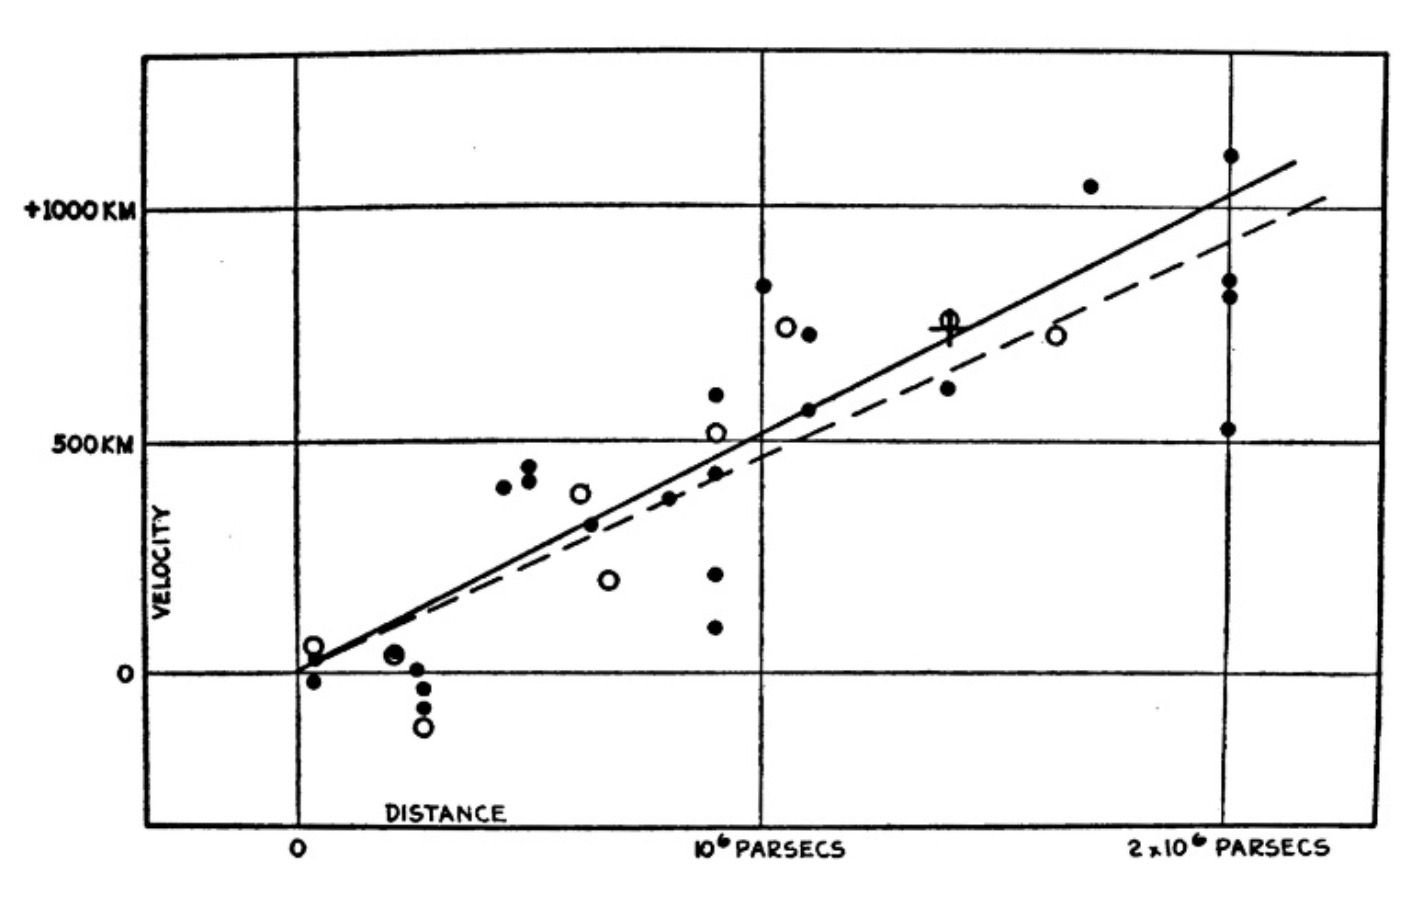
\includegraphics[width=0.9\columnwidth]{figures/hubble_original.png}
%\fbox{\parbox{0.8\textwidth}{\centering\vspace{2cm}\textit{Figure placeholder: Hubble's 1929 original velocity--distance diagram}\vspace{2cm}}}
%\caption{Hubble's 1929 velocity--distance diagram for nearby galaxies, providing the first observational evidence for a linear relation between recession velocity and distance.}
%\label{fig:hubble_1929}
%\end{figure}

As with many cases in science, the discovery was not named after its original discoverer. Two years before Hubble, in 1927, the Belgian Catholic priest, mathematician and astronomer Georges Lema\^{i}tre independently derived the velocity--distance relation from solutions of Einstein's field equations and estimated the proportionality constant from available data. The International Astronomical Union (IAU) now recommends the name \textbf{Hubble--Lema\^{i}tre law} in recognition of Lema\^{i}tre's contribution.

%\begin{figure}[H]
%\centering
% TODO: Add figure --- Lematre 1927 and Hubble 1929 diagrams side by side
%\fbox{\parbox{0.8\textwidth}{\centering\vspace{2cm}\textit{Figure placeholder: Lema\^{i}tre (1927) and Hubble (1929) diagrams side by side}\vspace{2cm}}}
%\caption{Left: Lema\^{i}tre's 1927 velocity--distance relation. Right: Hubble's 1929 version of the same relation. Both point to the same conclusion---the Universe is expanding.}
%\label{fig:lemaitre_hubble}
%\end{figure}

Seventy years of subsequent work dramatically refined the measurement. In 2001, Wendy Freedman and collaborators used the Hubble Space Telescope Key Project to calibrate distances to nearby galaxies and found $\Hnot = 70 \pm 7\kmsMpc$, consistent with the modern best estimates.

\begin{figure}[H]
\centering
% TODO: Add figure --- Freedman et al. (2001) Hubble diagram
%\fbox{\parbox{0.8\textwidth}{\centering\vspace{2cm}\textit{Figure placeholder: Freedman et al.\ (2001) HST Key Project Hubble diagram}\vspace{2cm}}}
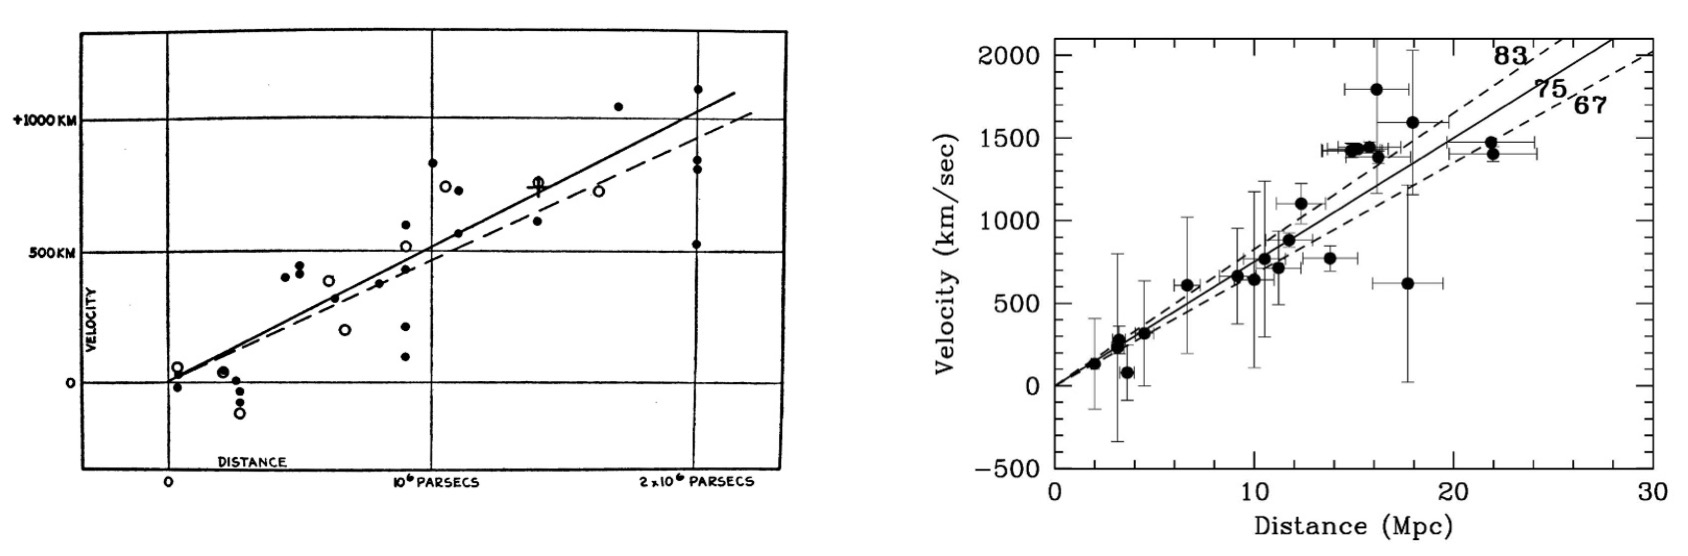
\includegraphics[width=0.9\columnwidth]{figures/hubble_modern.png}
\caption{{\em Left: } Hubble's 1929 velocity--distance diagram for nearby galaxies, providing the first observational evidence for a linear relation between recession velocity and distance. {\em Right:} The Hubble diagram from the HST Key Project (Freedman et al.\ 2001), yielding $\Hnot = 70 \pm 7\kmsMpc$ from multiple distance indicators.}
\label{fig:freedman_2001}
\end{figure}


% ===================================================================
\section{The Scale Factor and Homogeneous Expansion}
\label{sec:scale_factor}
% ===================================================================

Hubble's law tells us that galaxies are receding from us with velocities proportional to their distance. At first glance, this seems to place us at the centre of the Universe, violating the cosmological principle. The resolution is that the expansion is \emph{homogeneous and isotropic}: every observer, regardless of their location, sees the same Hubble law.

\subsection*{The Triangle Argument}

To see this concretely, consider three galaxies at positions $\vec{r}_1$, $\vec{r}_2$, and $\vec{r}_3$. The sides of the triangle they form are
\begin{equation}
    r_{12} = |\vec{r}_1 - \vec{r}_2|, \qquad r_{23} = |\vec{r}_2 - \vec{r}_3|, \qquad r_{31} = |\vec{r}_3 - \vec{r}_1|\,.
\end{equation}
A homogeneous and isotropic expansion must preserve the shape of this triangle---that is, the ratios of the side lengths must remain constant. The only expansion law compatible with this requirement is
\begin{equation}
    r_{12}(t) = a(t)\,r_{12}(t_0), \qquad r_{23}(t) = a(t)\,r_{23}(t_0), \qquad r_{31}(t) = a(t)\,r_{31}(t_0),
\label{eq:scale_factor_triangle}
\end{equation}
where $a(t)$ is a universal function of time called the \textbf{scale factor}, normalised so that $a(t_0) = 1$ at the present epoch~$t_0$. The scale factor is independent of both position and direction---it encodes the entire expansion history of the Universe.

\begin{figure}[H]
\centering
% TODO: Add figure --- Homogeneous expansion triangle / balloon analogy
%\fbox{\parbox{0.8\textwidth}{\centering\vspace{2cm}\textit{Figure placeholder: Homogeneous expansion of a triangle of galaxies}\vspace{2cm}}}
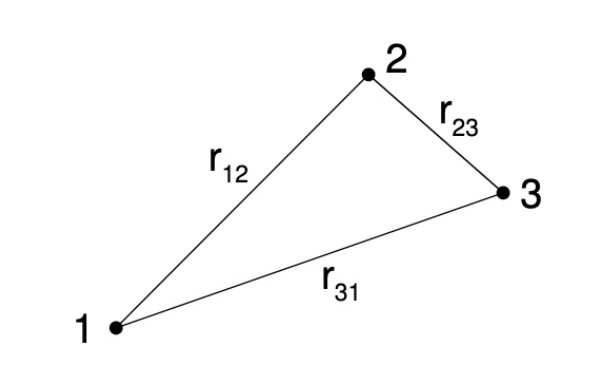
\includegraphics[width=0.6\columnwidth]{figures/triangle.png}
\caption{Illustration of homogeneous expansion: a triangle of galaxies at two different times. All inter-galaxy distances are rescaled by the same factor $a(t)$, preserving the shape of the triangle.}
\label{fig:expansion_triangle}
\end{figure}

\subsection*{Deriving Hubble's Law from the Scale Factor}

At any time $t$, an observer in galaxy~1 sees galaxy~2 receding with velocity
\begin{equation}
    v_{12}(t) = \frac{\dd r_{12}}{\dd t} = \dot{a}(t)\,r_{12}(t_0) = \frac{\dot{a}}{a}\,r_{12}(t)\,.
\end{equation}
The same applies to any pair of galaxies. Defining the \textbf{Hubble parameter}
\begin{equation}
\boxed{H(t) \equiv \frac{\dot{a}(t)}{a(t)}\,,}
\label{eq:hubble_parameter}
\end{equation}
we recover the general form of Hubble's law: $v = H(t)\,r$. Evaluated at the present time, $H(t_0) \equiv \Hnot$ is the \textbf{Hubble constant}. Crucially, an observer in any galaxy derives exactly the same Hubble law with the same value of~$H$, consistent with the cosmological principle.

\subsection*{General Relativity and the Friedmann Equations}

The mathematical framework that underpins the expanding universe is Einstein's General Theory of Relativity (1915), which describes gravity not as a force but as the curvature of spacetime caused by the presence of mass and energy. In 1917, Willem de Sitter found both static and expanding solutions to Einstein's field equations, though Einstein and de Sitter initially preferred the static case. In 1922, Alexander Friedmann derived the general non-static solutions describing universes that can expand or contract---pointing out an error in Einstein's earlier analysis. We will derive these \textit{Friedmann equations} in full detail in Chapter~\ref{ch:background_dynamics}.


% ===================================================================
\section{Big Bang vs.\ Steady State}
\label{sec:bb_vs_ss}
% ===================================================================

Hubble's discovery of the expanding Universe was a major advance, but it did not immediately settle the question of the Universe's origin. Two competing models emerged:

\begin{itemize}
    \item \textbf{The Hot Big Bang Model} (Hubble, Lema\^{i}tre): The Universe began in an extremely hot, dense state and has been expanding and cooling ever since. The cosmological principle holds, but the Universe evolves with time---its temperature, density, and composition all change.
    \item \textbf{The Steady State Model} (Bondi, Gold, and Hoyle, 1948): The Universe obeys a ``perfect cosmological principle''---it is homogeneous and isotropic not only in space but also in time. Although it expands, matter is continuously created to maintain a constant average density.
\end{itemize}

\begin{figure}[H]
\centering
% TODO: Add figure --- Big Bang vs Steady State schematic
%\fbox{\parbox{0.8\textwidth}{\centering\vspace{2cm}\textit{Figure placeholder: Schematic comparison of the Hot Big Bang and Steady State models}\vspace{2cm}}}
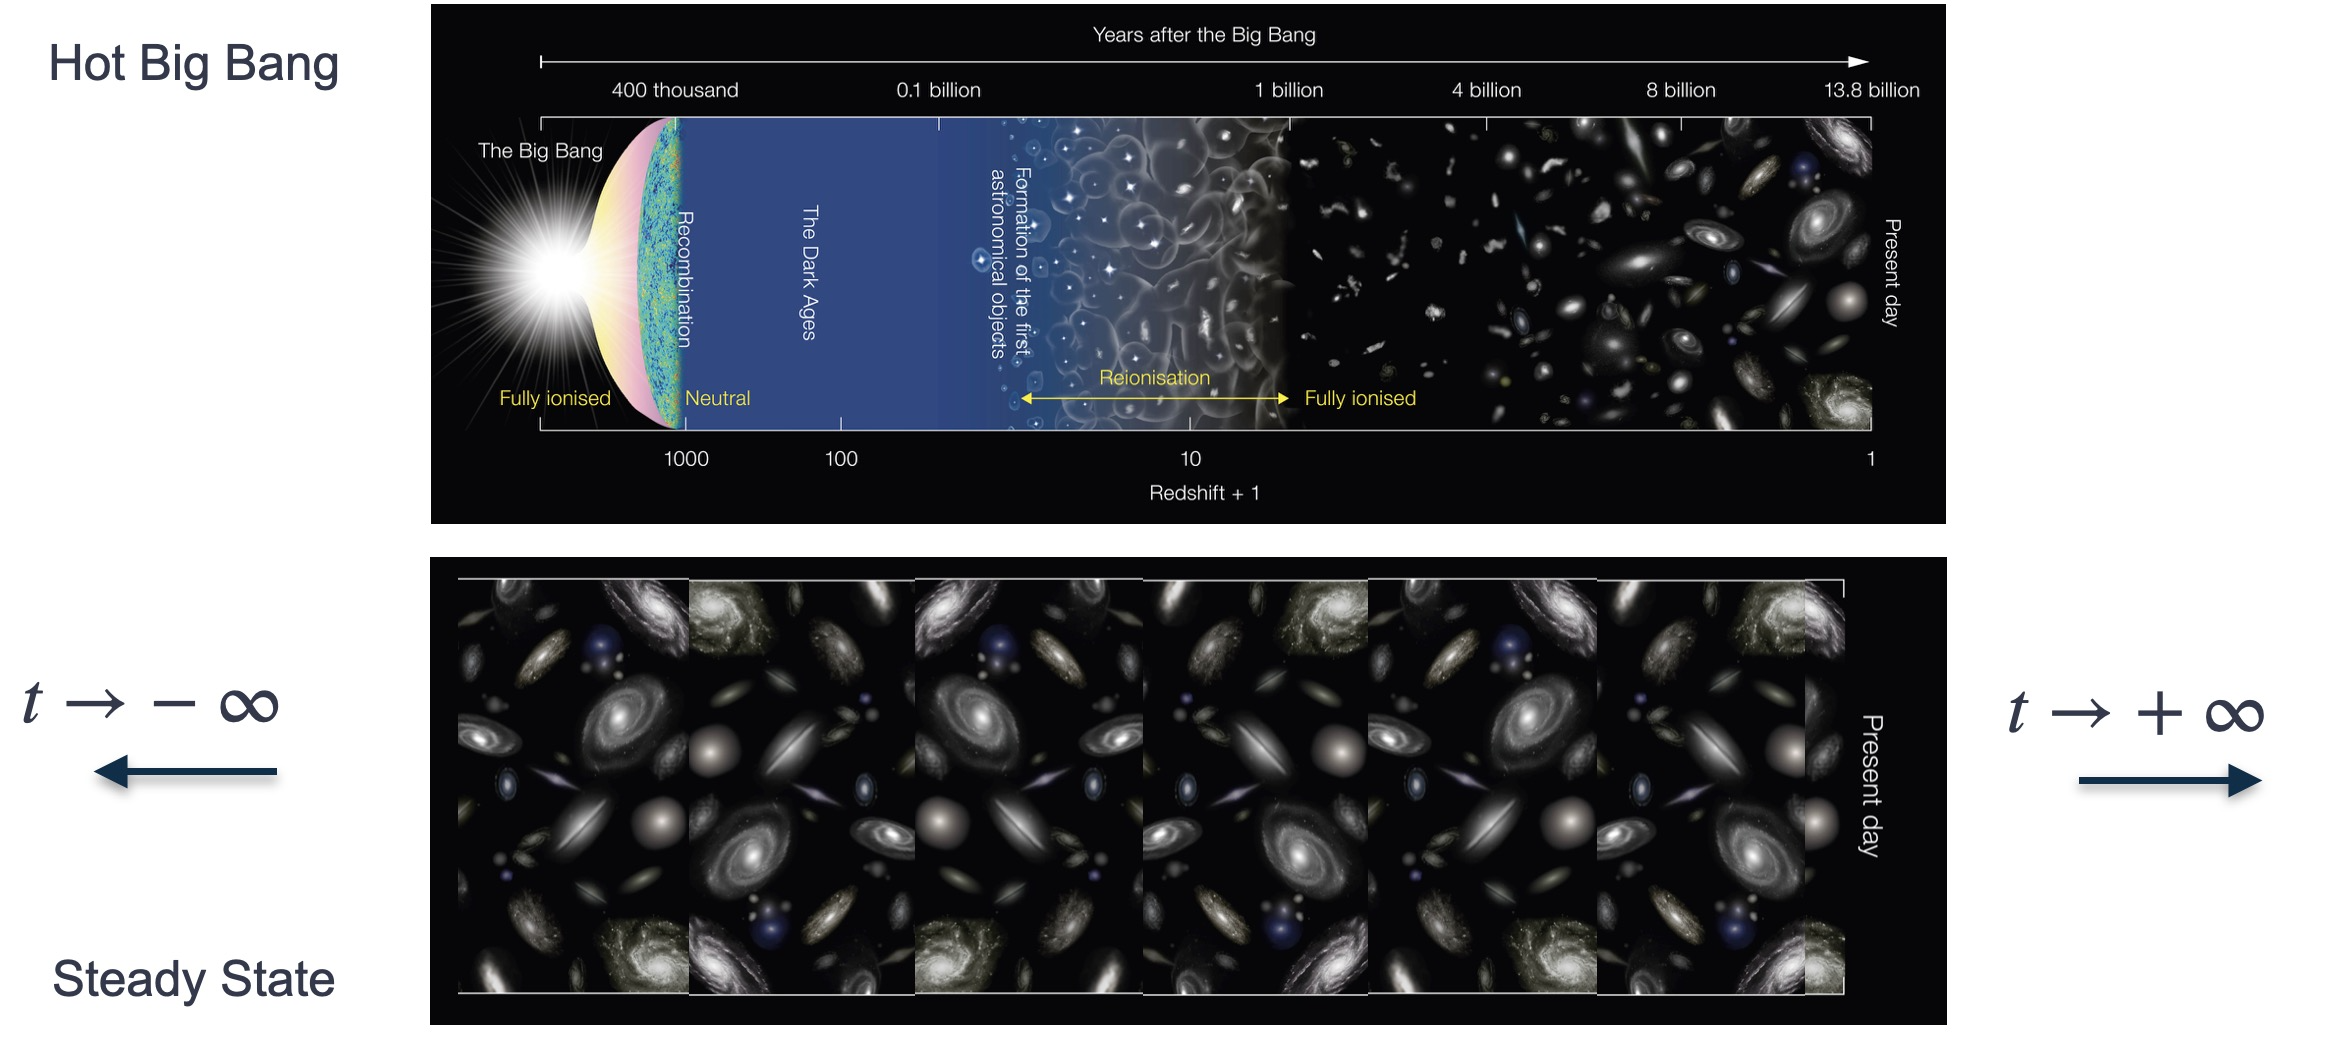
\includegraphics[width=\columnwidth]{figures/big_bang_steady_state.png}
\caption{Schematic comparison of the Hot Big Bang and Steady State models. In the Big Bang model, the Universe has a finite age and evolves from an initial singularity. In the Steady State model, the Universe has existed forever in roughly the same state, with continuous matter creation compensating for the dilution due to expansion.}
\label{fig:bb_vs_ss}
\end{figure}

Through the 1950s and 1960s, the ``Great Debate'' shifted to the question of which model correctly described our Universe. Several observations ultimately ruled out the Steady State model:
\begin{enumerate}
    \item \textbf{Quasar evolution} (M.~Schmidt 1963; M.~Rees and D.~Sciama 1965): The abundance of quasars (quasi-stellar objects) at high redshift is much larger than at low redshift, violating the time symmetry required by the perfect cosmological principle.
    \item \textbf{The Cosmic Microwave Background} (A.~Penzias and R.~Wilson 1965): The discovery of a pervasive thermal radiation field at $T\approx 3\,\mathrm{K}$, naturally explained as the cooled remnant of the hot early Universe, had no satisfactory explanation in the Steady State framework.
    \item \textbf{Singularity theorems} (S.~Hawking and G.~Ellis 1966): On purely theoretical grounds, Hawking showed that any plausible general-relativistic cosmology satisfying reasonable energy conditions must contain an initial singularity, undermining the premise of an eternal, unchanging Universe.
\end{enumerate}

Together, these observations and theoretical results firmly established the Hot Big Bang as the standard model of cosmology.


% ===================================================================
\section{Discovery of the Cosmic Microwave Background}
\label{sec:cmb_discovery}
% ===================================================================

The discovery of the cosmic microwave background (CMB) radiation is one of the most important events in the history of cosmology, providing direct evidence for the hot, dense early Universe predicted by the Big Bang model.

\subsection*{Penzias and Wilson (1965)}

In 1965, Arno Penzias and Robert Wilson, working at Bell Telephone Laboratories in Holmdel, New Jersey, were using a sensitive horn antenna---originally built for satellite communications---to survey the sky at microwave frequencies. They cooled the receiver with liquid helium to suppress thermal noise from the detector itself. Despite meticulous elimination of all known sources of interference (including removing what they diplomatically described as a ``white dielectric material'' deposited by pigeons nesting in the antenna), they found a persistent, isotropic background signal corresponding to an antenna temperature of approximately $3.5\,\mathrm{K}$ at a wavelength of $7.35\,\mathrm{cm}$.

At the same time and by coincidence, Jim Peebles at Princeton University had independently predicted the existence of a cosmic background radiation as a relic of the hot early Universe. When Penzias contacted the Princeton group, Robert Dicke, Peter Roll, and David Wilkinson visited Bell Labs to examine the data and the experimental setup. Once convinced of the result, the two groups published companion papers in the \textit{Astrophysical Journal} (volume 142):
\begin{itemize}
    \item Dicke, Peebles, Roll \& Wilkinson: ``Cosmic Black-Body Radiation'' (theoretical interpretation).
    \item Penzias \& Wilson: ``A Measurement of Excess Antenna Temperature at 4080~Mc/s'' (observational detection).
\end{itemize}
Penzias and Wilson were awarded the Nobel Prize in Physics in 1978 for this discovery.

%\begin{figure}[H]
%\centering
% TODO: Add figure --- Penzias and Wilson with the horn antenna
%\fbox{\parbox{0.8\textwidth}{\centering\vspace{2cm}\textit{Figure placeholder: Penzias and Wilson with the Bell Labs horn antenna}\vspace{2cm}}}
%\caption{Arno Penzias and Robert Wilson standing in front of the horn antenna at Bell Telephone Laboratories, Holmdel, New Jersey, with which they discovered the cosmic microwave background radiation in 1965.}
%\label{fig:penzias_wilson}
%\end{figure}

Remarkably, the CMB may have been observed even earlier. In 1940, Andrew McKellar detected excited rotational states of cyanogen (CN) molecules in interstellar space, corresponding to an excitation temperature of approximately $2.3\,\mathrm{K}$. Walter Adams confirmed similar observations in 1941. These measurements were not, however, interpreted as evidence for a cosmic radiation background at the time.

\subsection*{The Search for Anisotropies}

If the large-scale structure we observe today---galaxies, clusters, voids, and filaments---grew from small initial fluctuations by gravitational instability, then these seed fluctuations must also be imprinted on the CMB. Throughout the 1970s and 1980s, numerous experiments searched for temperature anisotropies in the CMB but found none at increasing levels of sensitivity.

\subsection*{COBE, WMAP, and Planck}

In 1989, NASA launched the \textbf{Cosmic Background Explorer} (COBE) satellite, which carried two instruments of particular importance:
\begin{itemize}
    \item \textbf{FIRAS} (Far InfraRed Absolute Spectrophotometer): Measured the CMB frequency spectrum with extraordinary precision, confirming that it is a near-perfect blackbody at $T = 2.725 \pm 0.002\,\mathrm{K}$.
    \item \textbf{DMR} (Differential Microwave Radiometer): Detected for the first time the tiny temperature anisotropies in the CMB at the level of $\Delta T/T \sim 10^{-5}$, corresponding to fluctuations of order $\pm 30\,\mu\mathrm{K}$.
\end{itemize}
George Smoot and John Mather were awarded the Nobel Prize in Physics in 2006 for these measurements.

Subsequent space missions dramatically improved the angular resolution of CMB maps and added measurements of polarisation:
\begin{itemize}
    \item \textbf{WMAP} (Wilkinson Microwave Anisotropy Probe, 2001--2010): Provided full-sky temperature and polarisation maps with angular resolution of approximately $0.2^{\circ}$.
    \item \textbf{Planck} (2009--2013): Achieved even higher resolution ($\sim 5'$) and sensitivity across nine frequency bands, delivering the most precise measurements of the CMB temperature and polarisation power spectra to date, along with tight constraints on the cosmological parameters of the $\Lcdm$ model.
\end{itemize}
These missions ushered in the era of \textit{precision cosmology}, in which the fundamental parameters of the Universe are determined to percent-level accuracy. We will study the physics of CMB anisotropies in detail in Chapter~\ref{ch:cmb}.

\begin{figure}[H]
\centering
% TODO: Add figure --- COBE/WMAP/Planck maps comparison
%\fbox{\parbox{0.8\textwidth}{\centering\vspace{2cm}\textit{Figure placeholder: Progression of CMB temperature maps from COBE to WMAP to Planck}\vspace{2cm}}}
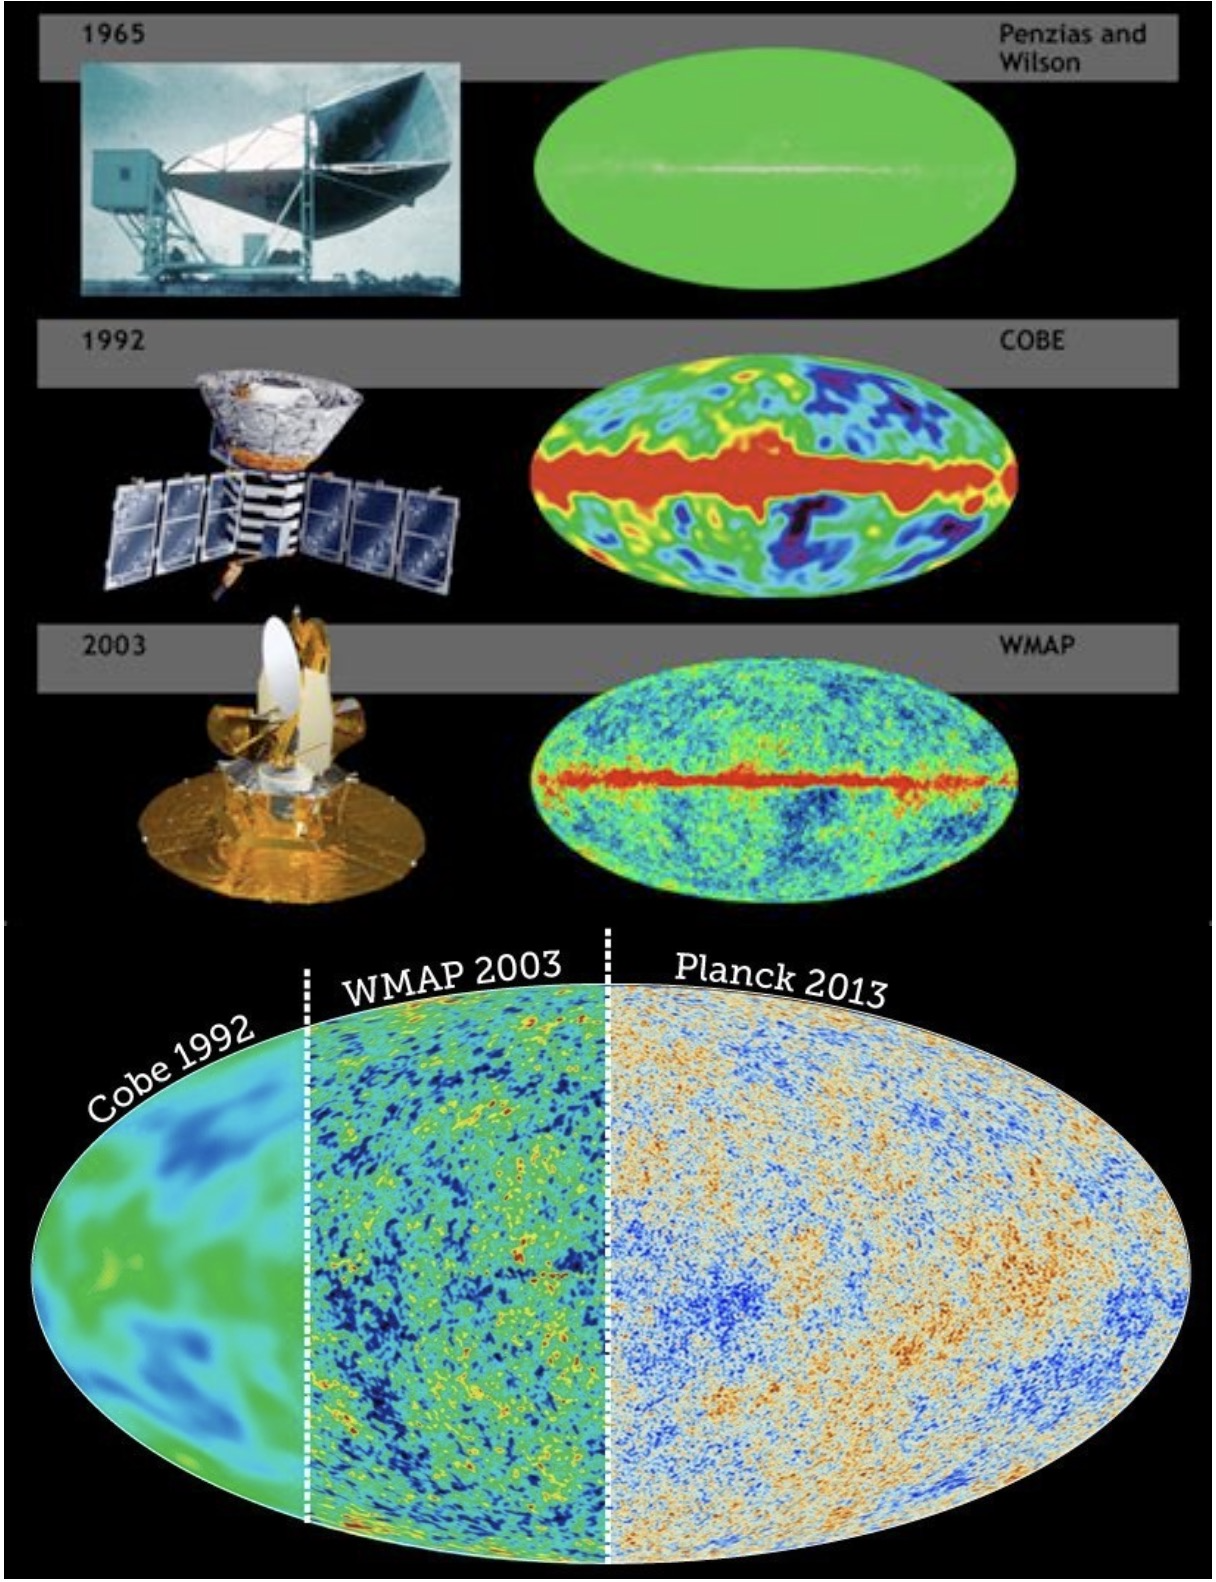
\includegraphics[width=0.5\columnwidth]{figures/cobe_wmap_planck.png}
\caption{The progression of CMB temperature anisotropy maps from COBE (1992) through WMAP (2003) to Planck (2013), illustrating the dramatic improvement in angular resolution and sensitivity over two decades of space-based observations.}
\label{fig:cmb_progression}
\end{figure}


% ===================================================================
\section{Mapping the Universe with Galaxy Surveys}
\label{sec:galaxy_surveys}
% ===================================================================

While the CMB provides a snapshot of the Universe at a redshift of $z\approx 1100$, galaxy redshift surveys map the three-dimensional distribution of matter in the more recent Universe. Constructing a redshift survey is a two-step process: first, a wide-field imaging survey identifies galaxies above a defined brightness limit; then, spectroscopic observations measure the redshifts of the selected galaxies.

\subsection*{Early Surveys and the Discovery of Cosmic Structure}

The first systematic redshift survey was the \textbf{CfA Redshift Survey}, begun in 1977 at the Center for Astrophysics. Its initial catalogue of approximately 2{,}200 galaxies, completed in 1982, was later extended to the CfA2 survey of 18{,}000 galaxies by John Huchra and Margaret Geller in the early 1990s. These pioneering surveys revealed that galaxies are not uniformly distributed, but instead trace a complex ``cosmic web'' of filaments, walls, and clusters surrounding large, nearly empty voids.

\begin{figure}[H]
\centering
% TODO: Add figure --- CfA redshift survey "stickman" map
%\fbox{\parbox{0.8\textwidth}{\centering\vspace{2cm}\textit{Figure placeholder: The CfA redshift survey slice showing the cosmic web}\vspace{2cm}}}
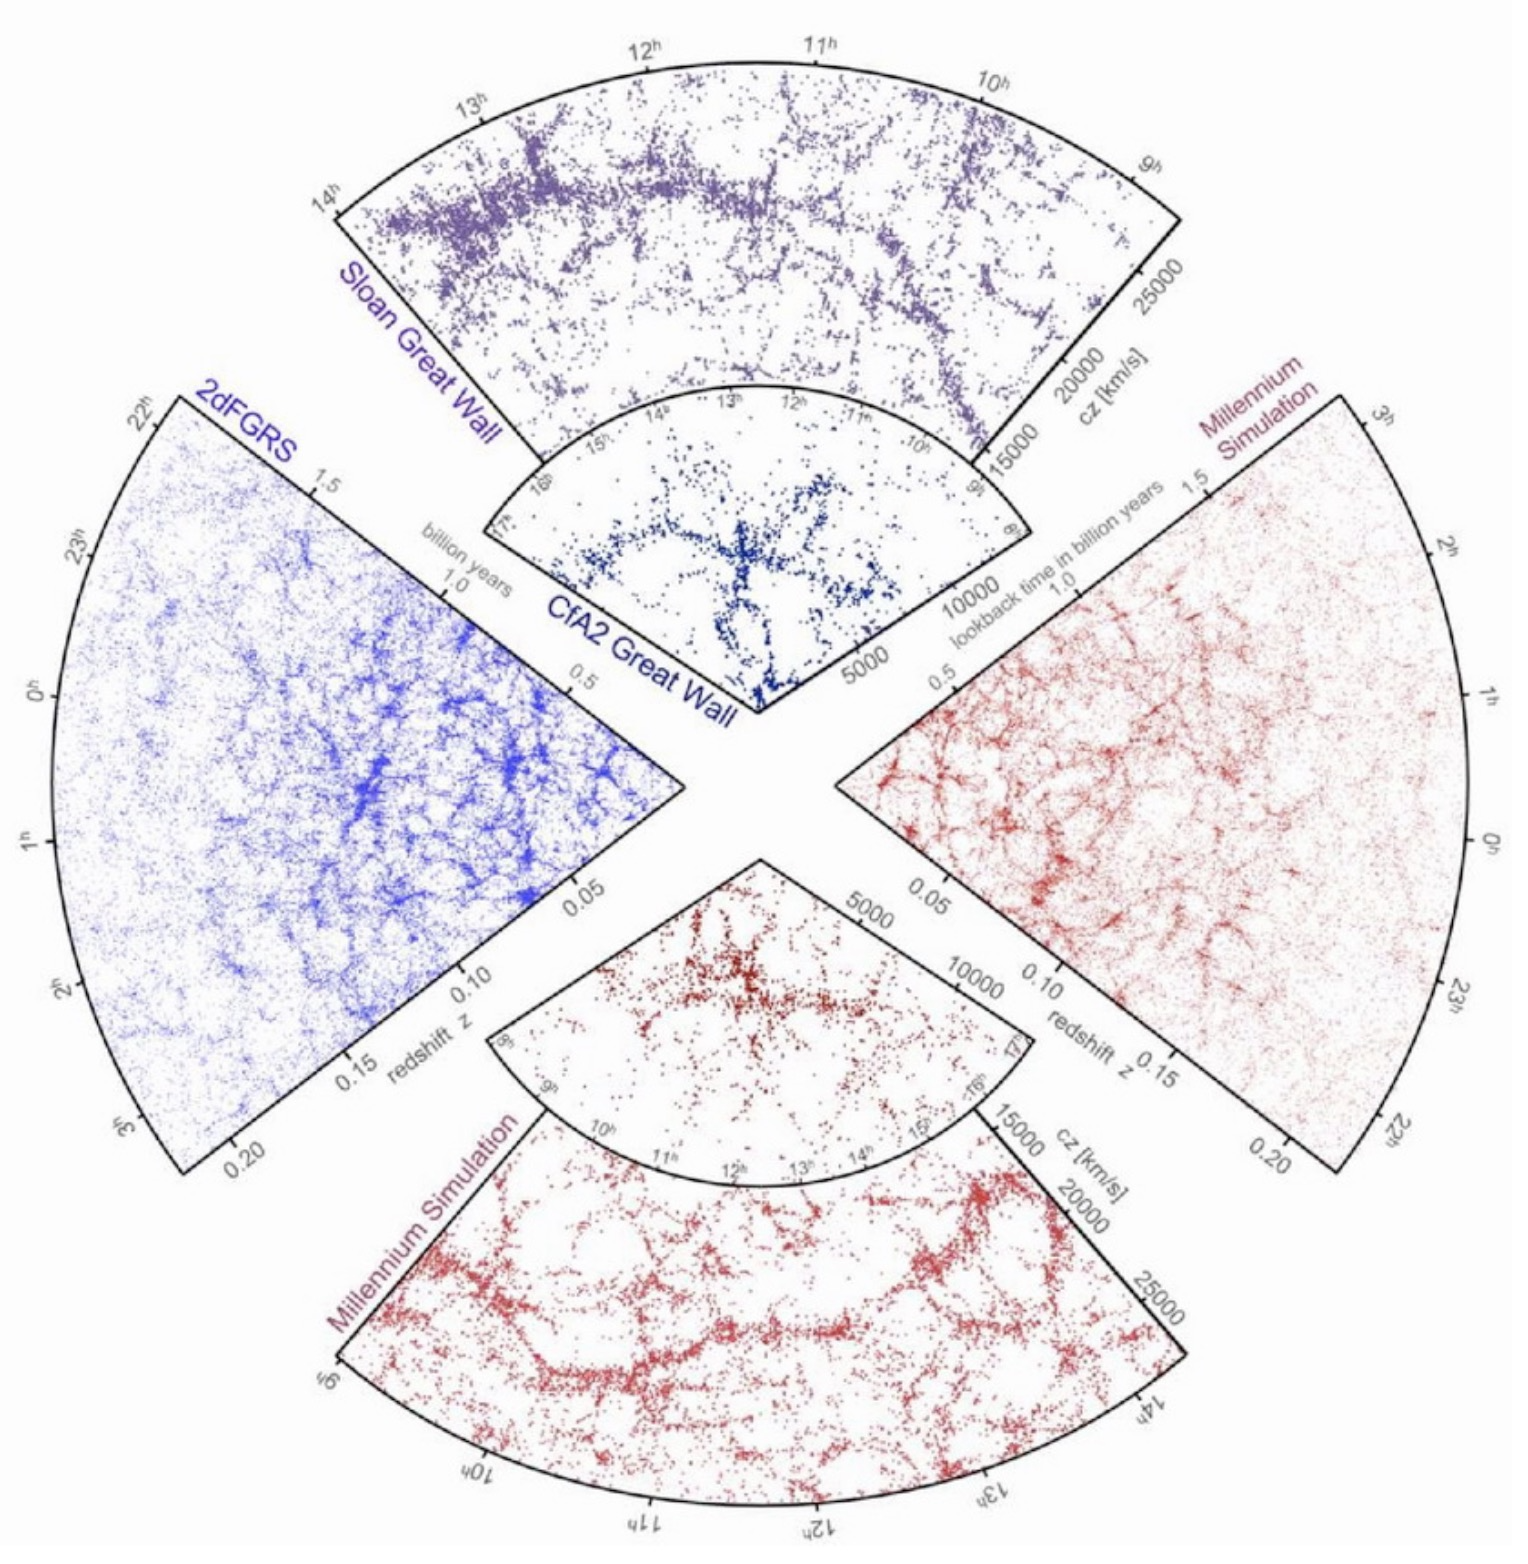
\includegraphics[width=0.6\columnwidth]{figures/2df_sdss.png}
\caption{A slice of the CfA2 redshift survey, revealing the filamentary large-scale structure of the Universe. Galaxies cluster on the surfaces of bubble-like voids.}
\label{fig:cfa_survey}
\end{figure}

\subsection*{The Multi-Fibre Revolution}

Early redshift surveys were limited by the need to observe one galaxy at a time. From the 1990s onwards, the development of fibre-optic multi-object spectrographs enabled the simultaneous measurement of hundreds of galaxy spectra, making much larger surveys feasible. Notable examples include:
\begin{itemize}
    \item \textbf{2dFGRS} (Two-degree-Field Galaxy Redshift Survey): 221{,}000 galaxy redshifts, completed in 2002.
    \item \textbf{SDSS} (Sloan Digital Sky Survey): The first large digital imaging and spectroscopic survey, which has mapped millions of galaxies and quasars since 2000.
\end{itemize}

In 2005, the 2dFGRS and SDSS collaborations independently reported the detection of the \textbf{baryon acoustic oscillation} (BAO) signal in the galaxy power spectrum---a characteristic scale imprinted by sound waves in the primordial plasma, providing a ``standard ruler'' for measuring cosmic distances. This opened a powerful new avenue for constraining the expansion history (see Chapter~\ref{ch:bao} for a detailed treatment).

\subsection*{BOSS, eBOSS, and DESI}

The SDSS programme continued with the \textbf{BOSS} (Baryon Oscillation Spectroscopic Survey, 2009--2014) and \textbf{eBOSS} (extended BOSS, 2014--2019) programmes, mapping the galaxy distribution across 11 billion years of cosmic history.

The current state of the art is the \textbf{Dark Energy Spectroscopic Instrument} (DESI), which began survey operations in 2021 and aims to measure approximately 35 million galaxy and quasar spectra---roughly ten times more than all previous surveys combined. DESI targets include luminous red galaxies (LRGs), emission line galaxies (ELGs), quasars (QSOs), and a bright galaxy survey (BGS), spanning a wide range of redshifts.

\begin{figure}[H]
\centering
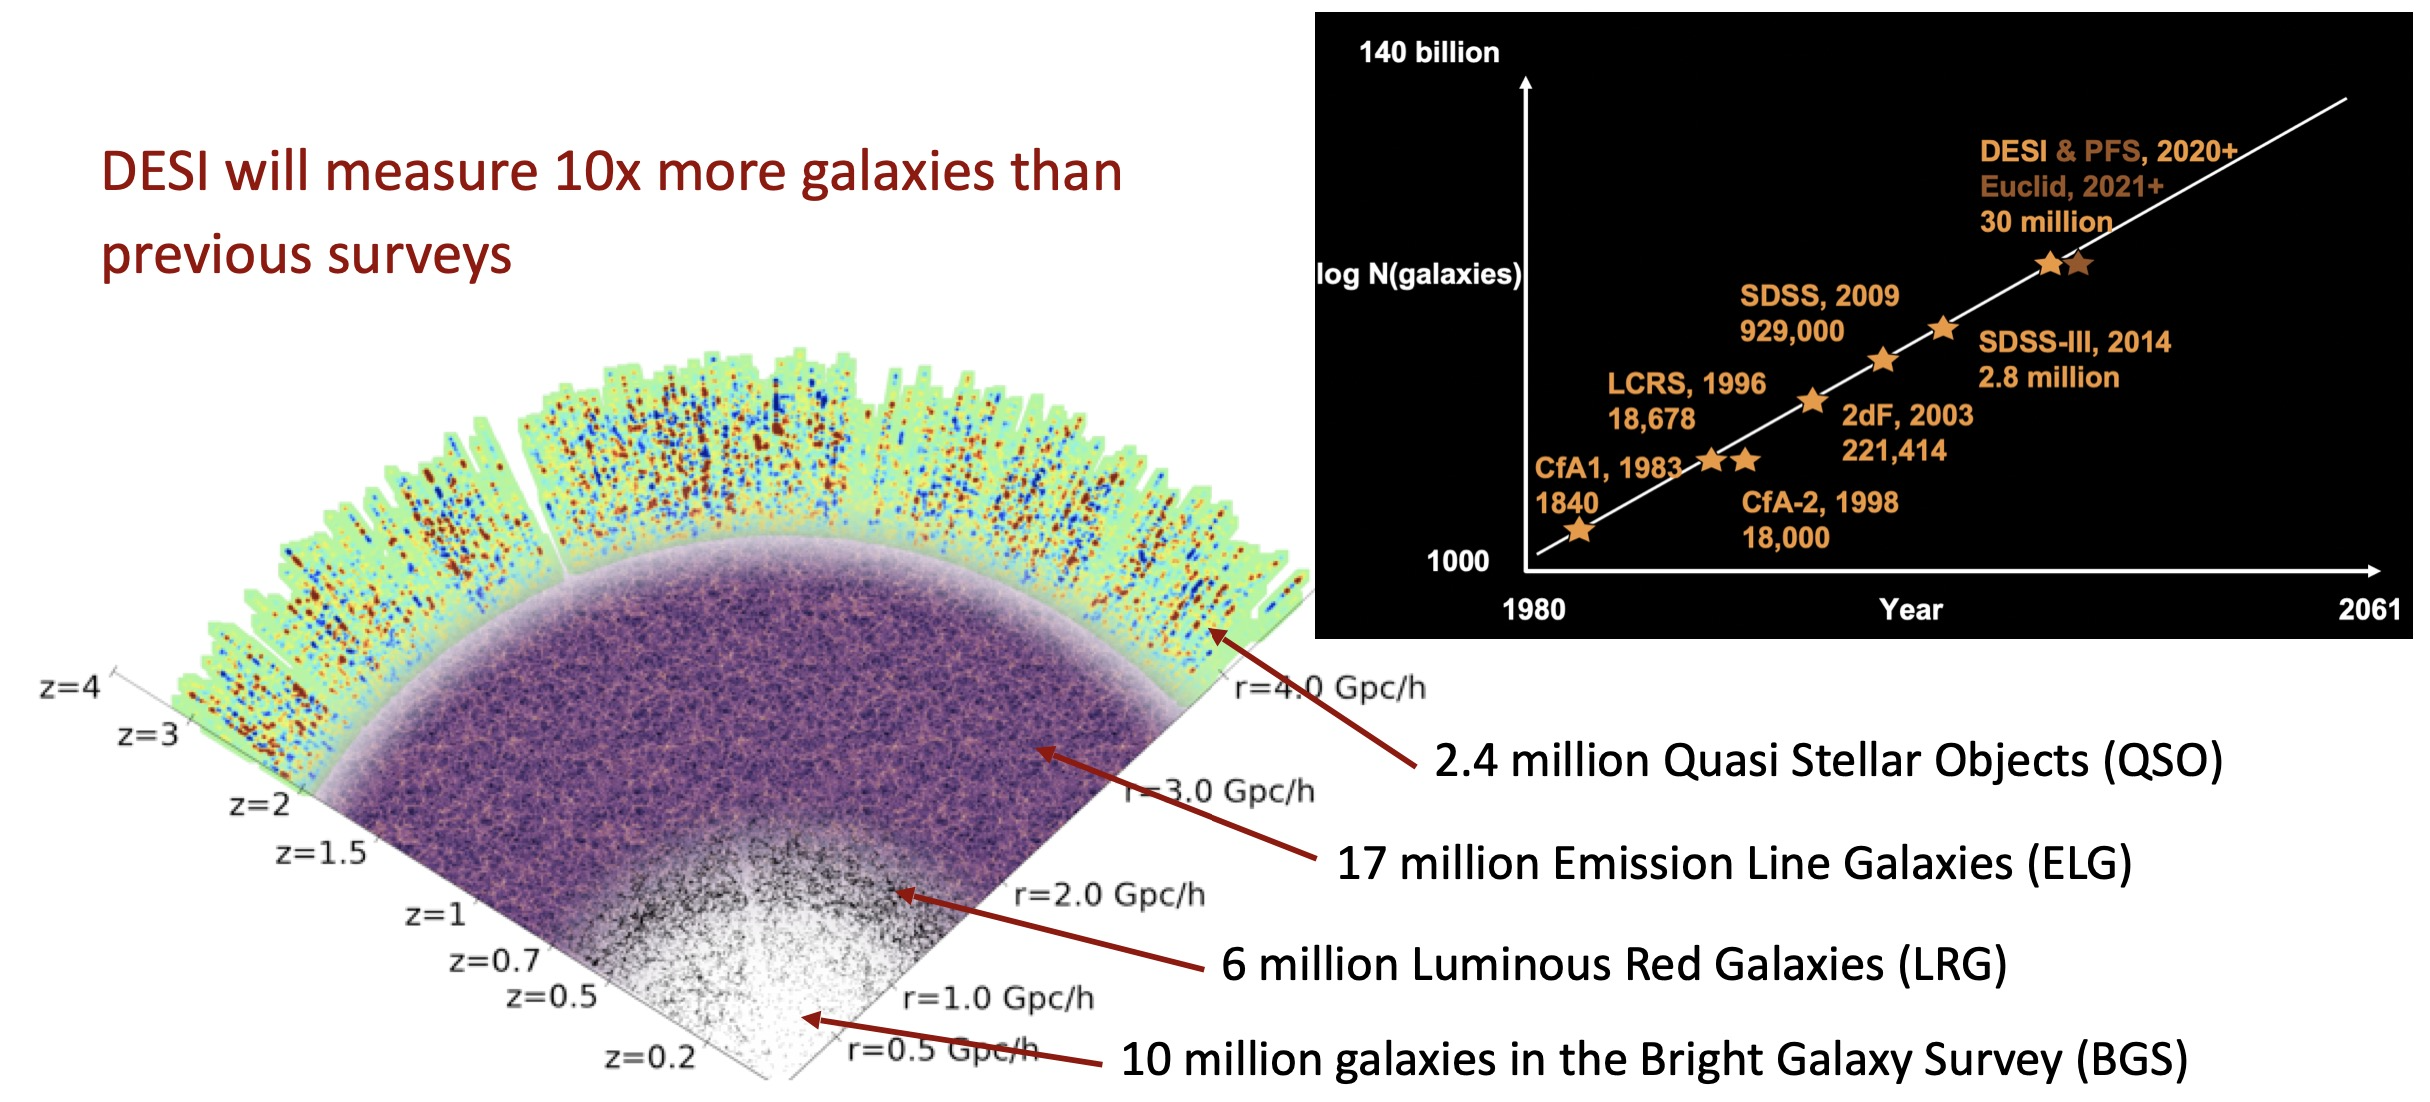
\includegraphics[width=0.8\columnwidth]{figures/desi.png}
\caption{A visualisation of the DESI survey volume, showing the distribution of different galaxy populations (LRGs, ELGs, QSOs) across redshift. DESI will measure approximately 35 million spectra, providing unprecedented precision on the expansion history and growth of structure.}
\label{fig:desi_survey}
\end{figure}


% ===================================================================
\section{Evidence for Dark Matter}
\label{sec:dark_matter_evidence}
% ===================================================================

The current cosmological picture requires two mysterious components that together account for roughly 95\% of the energy content of the Universe: dark matter and dark energy. We begin with the observational evidence for dark matter.

\subsection*{Galaxy Clusters and the Virial Theorem}

The first evidence for dark matter came from \textbf{Fritz Zwicky}'s study of the Coma Cluster (Abell~1656) in 1933. The Coma Cluster contains over 1{,}000 identified galaxies, and Zwicky measured their line-of-sight velocity dispersion. Applying the virial theorem, which relates the time-averaged kinetic and potential energies of a gravitationally bound system,
\begin{equation}
    \langle T \rangle = -\frac{1}{2}\langle U \rangle \quad\Longrightarrow\quad M \sim \frac{R\,\langle v^2\rangle}{G}\,,
\label{eq:virial}
\end{equation}
Zwicky estimated the total mass of the cluster and found it to be far larger than the luminous mass in its constituent galaxies. For the Coma Cluster, with a characteristic radius $R\approx 10^{23}\,\mathrm{m}$ and velocity dispersion $\langle v^2\rangle^{1/2}\approx 2\times 10^{6}\,\mathrm{m\,s^{-1}}$:
\begin{equation}
\boxed{M \approx \frac{R\,\langle v^2\rangle}{G} \sim \frac{2\times 10^{23}\times 4\times 10^{12}}{6.7\times 10^{-11}} \sim 10^{46}\,\mathrm{kg} \sim 5\times 10^{15}\,\Msun\,.}
\label{eq:coma_mass}
\end{equation}
This is far more mass than can be accounted for by the visible galaxies. Zwicky concluded that the cluster must be held together by some unseen ``dunkle Materie'' (dark matter). It would take approximately fifty years for the concept of dark matter to gain widespread acceptance.

\subsection*{Galaxy Rotation Curves}

In the late 1950s, observational hints emerged that stars in spiral galaxies were not moving as expected from Newtonian dynamics applied to the visible matter alone. In 1970, Vera Rubin, using a sensitive spectrograph developed by Kent Ford, measured the rotation velocities of stars at various distances from the centre of the Andromeda Galaxy (M31). For a galaxy whose mass is concentrated within radius $r$, Newtonian gravity predicts a Keplerian decline in the circular velocity:
\begin{equation}
    v_{\mathrm{circ}}(r) = \sqrt{\frac{GM(<r)}{r}} \;\propto\; r^{-1/2} \quad\text{(for $r$ beyond the luminous disc)}\,.
\end{equation}
Instead, Rubin found that rotation curves remain \textit{flat} ($v_{\mathrm{circ}}\approx\mathrm{const.}$) out to the largest measured radii, implying that $M(<r)\propto r$---the enclosed mass continues to grow linearly well beyond the visible disc. This is naturally explained by a massive, extended \textbf{dark matter halo} surrounding the galaxy.

\begin{figure}[H]
\centering
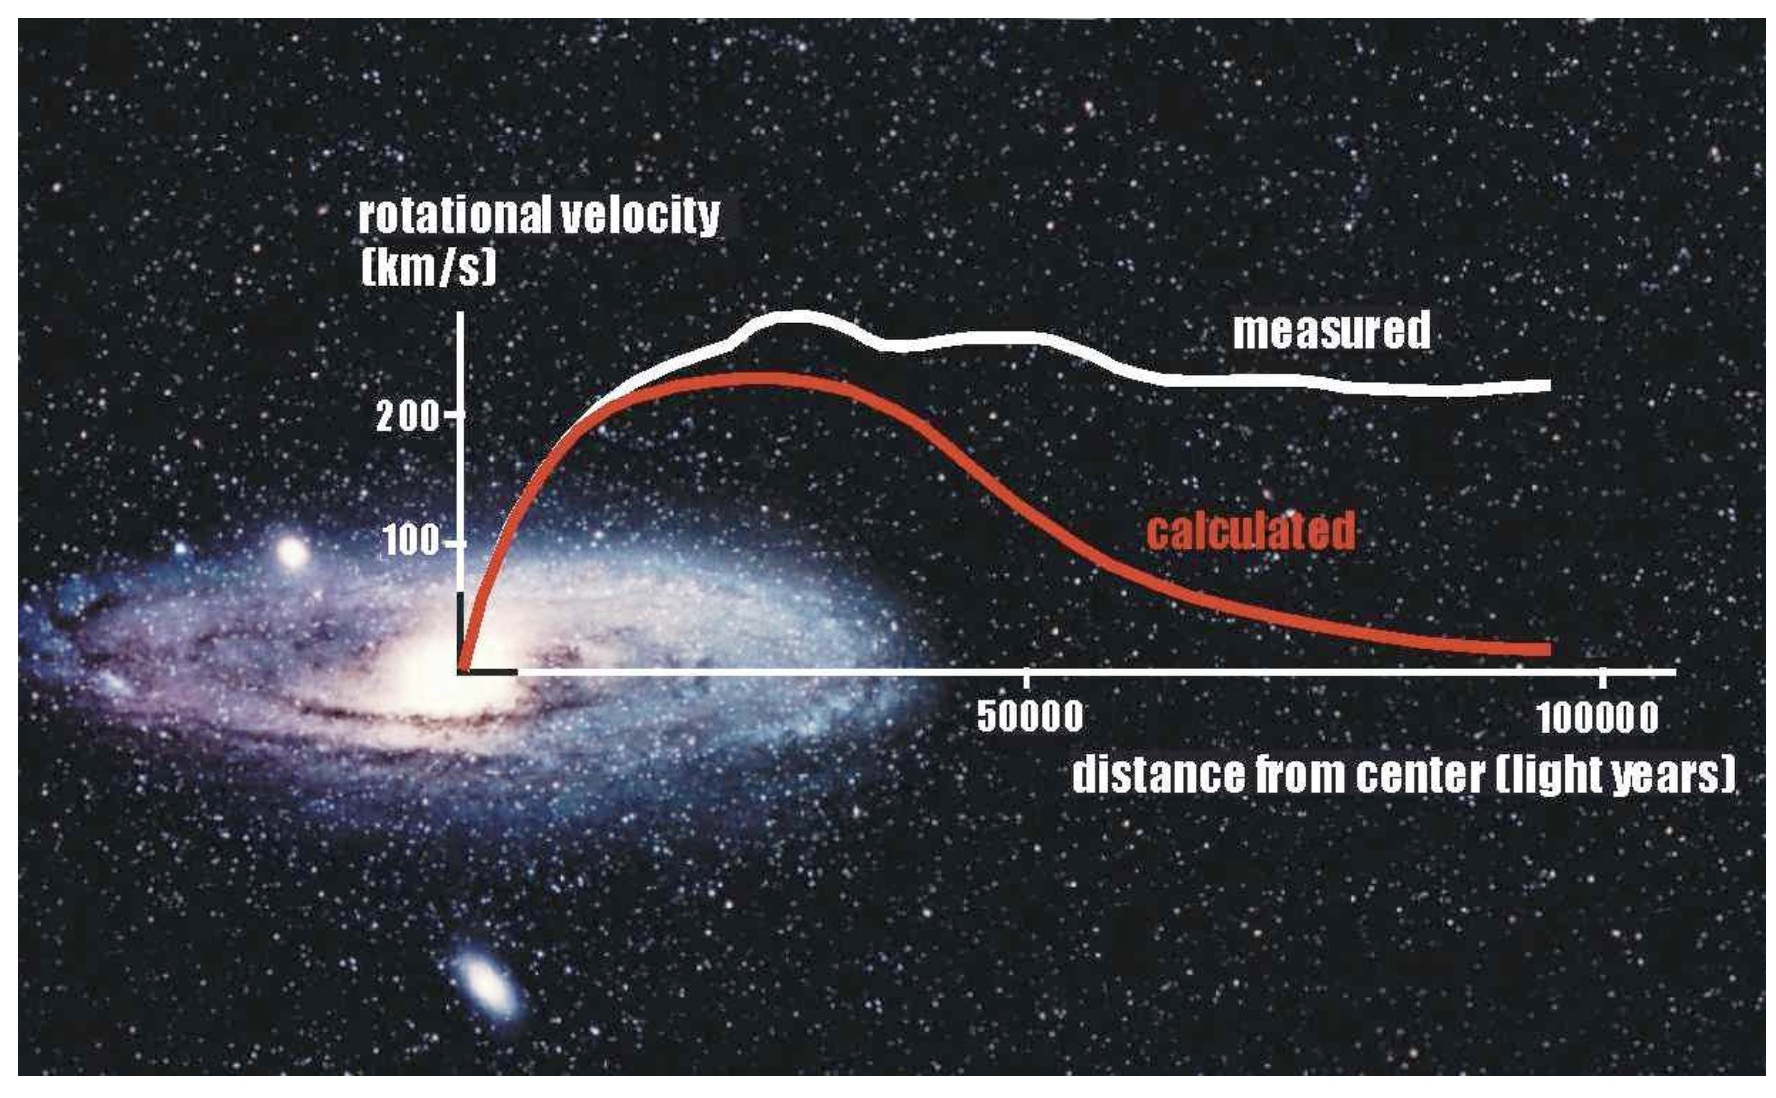
\includegraphics[width=0.6\columnwidth]{figures/rotation_curves.png}
\caption{Schematic galaxy rotation curve. The red line shows the expected Keplerian decline ($v\propto r^{-1/2}$) if only the visible disc mass were present. The white line shows the observed flat rotation curve, implying the existence of a dark matter halo whose enclosed mass grows linearly with radius.}
\label{fig:rotation_curve}
\end{figure}

\subsection*{Gravitational Lensing}

General relativity predicts that mass curves spacetime and deflects the paths of light rays. Massive objects such as galaxy clusters act as gravitational lenses, distorting the images of background galaxies. The strength of this lensing depends on the total projected mass along the line of sight, regardless of whether that mass is luminous or dark. Observations of both strong lensing (multiple images and arcs) around individual clusters and \textbf{weak lensing} (statistical distortions of the shapes of large samples of background galaxies) consistently require more mass than is observed in luminous matter, providing an independent confirmation of dark matter. We will study the physics of gravitational lensing in detail in Chapter~\ref{ch:gravitational_lensing}.

\begin{figure}[H]
\centering
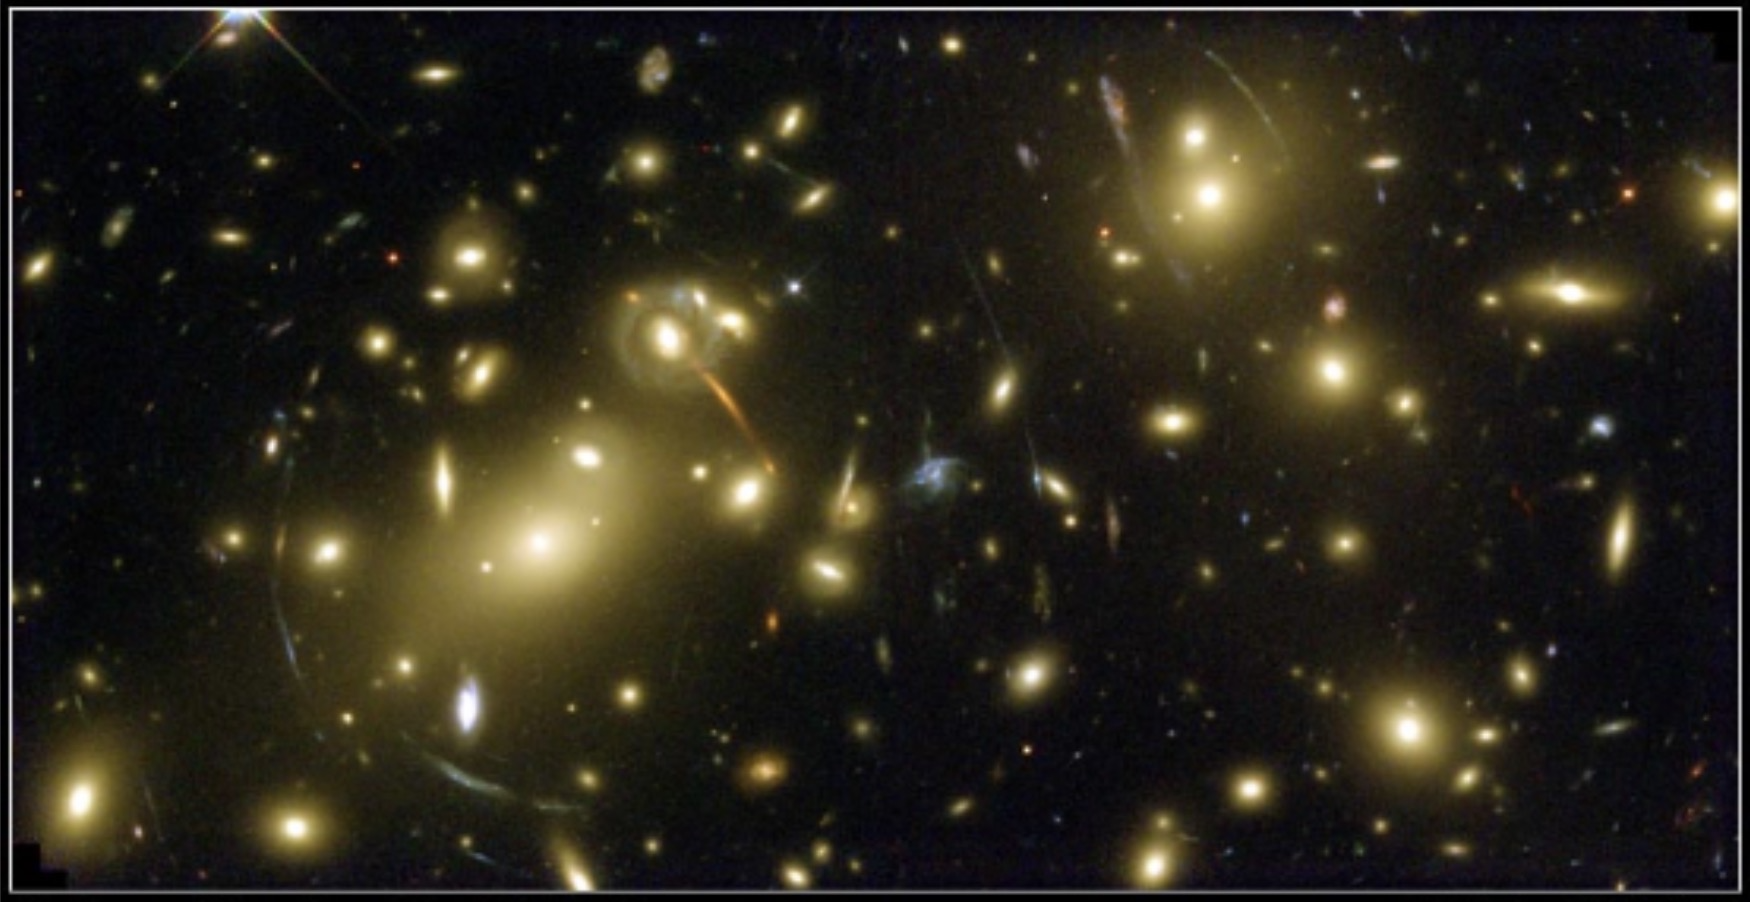
\includegraphics[width=0.7\columnwidth]{figures/abell_lensing.png}
\caption{Gravitational lensing by a massive galaxy cluster Abell 2218. The arcs visible around the cluster core are the distorted images of background galaxies, lensed by the cluster's gravitational field. The total lensing mass far exceeds the mass of the visible cluster galaxies and hot intracluster gas, providing strong evidence for dark matter.}
\label{fig:gravitational_lensing}
\end{figure}

\subsection*{The Cosmic Microwave Background}

The CMB provides yet another independent line of evidence for dark matter. In the early Universe, ordinary (baryonic) matter was ionised and interacted strongly with radiation through Thomson scattering, whereas dark matter interacts only gravitationally. These two components therefore evolve differently: baryons and photons form a tightly coupled fluid that supports acoustic oscillations, while dark matter perturbations grow freely under gravity, creating the gravitational potential wells into which the baryon--photon fluid falls.

This difference leaves a distinctive signature in the CMB power spectrum. Increasing the fraction of dark matter relative to baryonic matter changes the relative heights of the odd and even acoustic peaks. The Planck satellite's exquisite measurement of the CMB power spectrum constrains the dark matter density to $\Omc h^2 = 0.120 \pm 0.001$, roughly five times the baryon density $\Omb h^2 = 0.0224 \pm 0.0001$ (see Chapter~\ref{ch:cmb} for a full discussion).

%\begin{figure}[H]
%\centering
% TODO: Add figure --- CMB power spectrum with and without dark matter
%\fbox{\parbox{0.8\textwidth}{\centering\vspace{2cm}\textit{Figure placeholder: CMB temperature power spectrum with and without dark matter}\vspace{2cm}}}
%\caption{Comparison of the CMB temperature power spectrum in a universe with dark matter (left) and without dark matter (right). The presence of dark matter dramatically affects the relative heights and positions of the acoustic peaks.}
%\label{fig:cmb_dark_matter}
%\end{figure}


% ===================================================================
\section{Evidence for Dark Energy}
\label{sec:dark_energy_evidence}
% ===================================================================

\subsection*{Type Ia Supernovae}

Type Ia supernovae (SNe Ia) are thermonuclear explosions of white dwarf stars that reach a remarkably uniform peak luminosity, making them excellent ``standard candles'' for measuring cosmological distances. In 1998, two independent teams---the Supernova Cosmology Project and the High-$z$ Supernova Search Team---discovered that distant SNe Ia are systematically \emph{dimmer} than expected in a decelerating universe. The inescapable conclusion was that the expansion of the Universe is \emph{accelerating}, driven by an unknown component with negative pressure that has come to be called \textbf{dark energy}.

This discovery was awarded the Nobel Prize in Physics in 2011 (Saul Perlmutter, Brian Schmidt, and Adam Riess). It should be noted that there is ongoing investigation into potential systematic effects, in particular whether the peak brightness of SNe Ia correlates with the age of the host stellar population, which could affect cosmological inferences.

\begin{figure}[H]
\centering
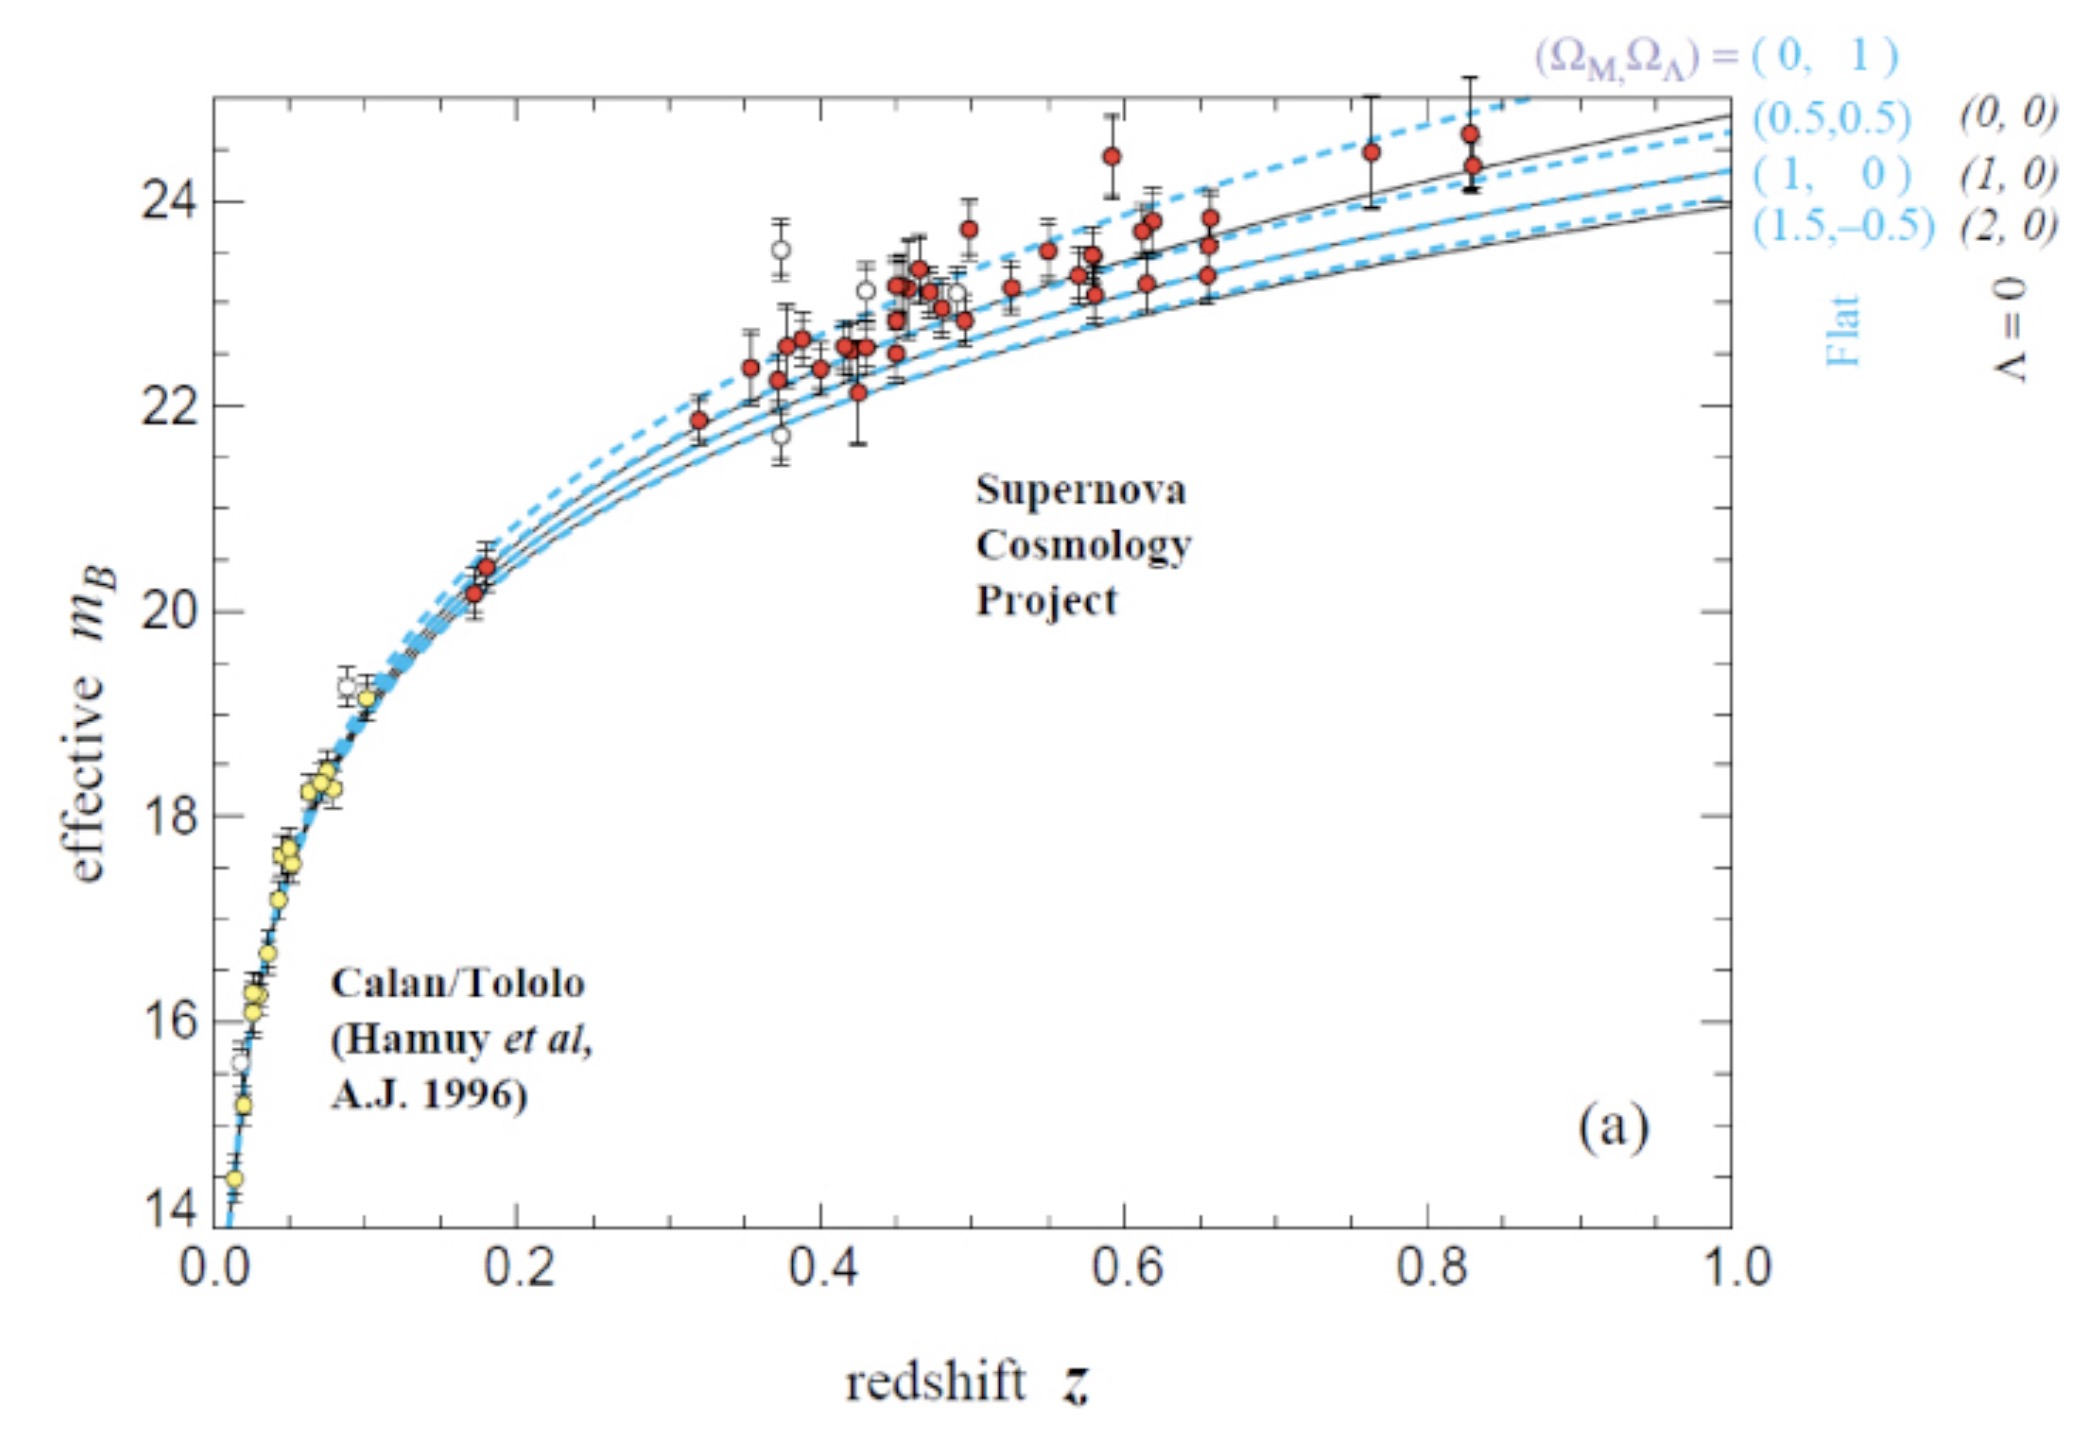
\includegraphics[width=0.6\columnwidth]{figures/supernovae_evidence.png}
\caption{The Hubble diagram for Type~Ia supernovae. Distant SNe~Ia are systematically fainter than expected in a matter-dominated, decelerating universe, providing direct evidence for the accelerating expansion.}
\label{fig:sn_hubble}
\end{figure}

\subsection*{CMB and the Geometry of Space}

Measurements of CMB anisotropies indicate that the Universe is spatially flat to high precision, meaning $\Omtot \approx 1$. However, the total amount of matter in the Universe (baryonic plus dark matter), as measured independently from the CMB power spectrum, accounts for only about 30\% of the critical density: $\Omm\approx 0.3$. For the Universe to be flat, the remaining $\sim 70\%$ must be supplied by an additional component: dark energy, with $\OmDE\approx 0.7$.

\begin{figure}[H]
\centering
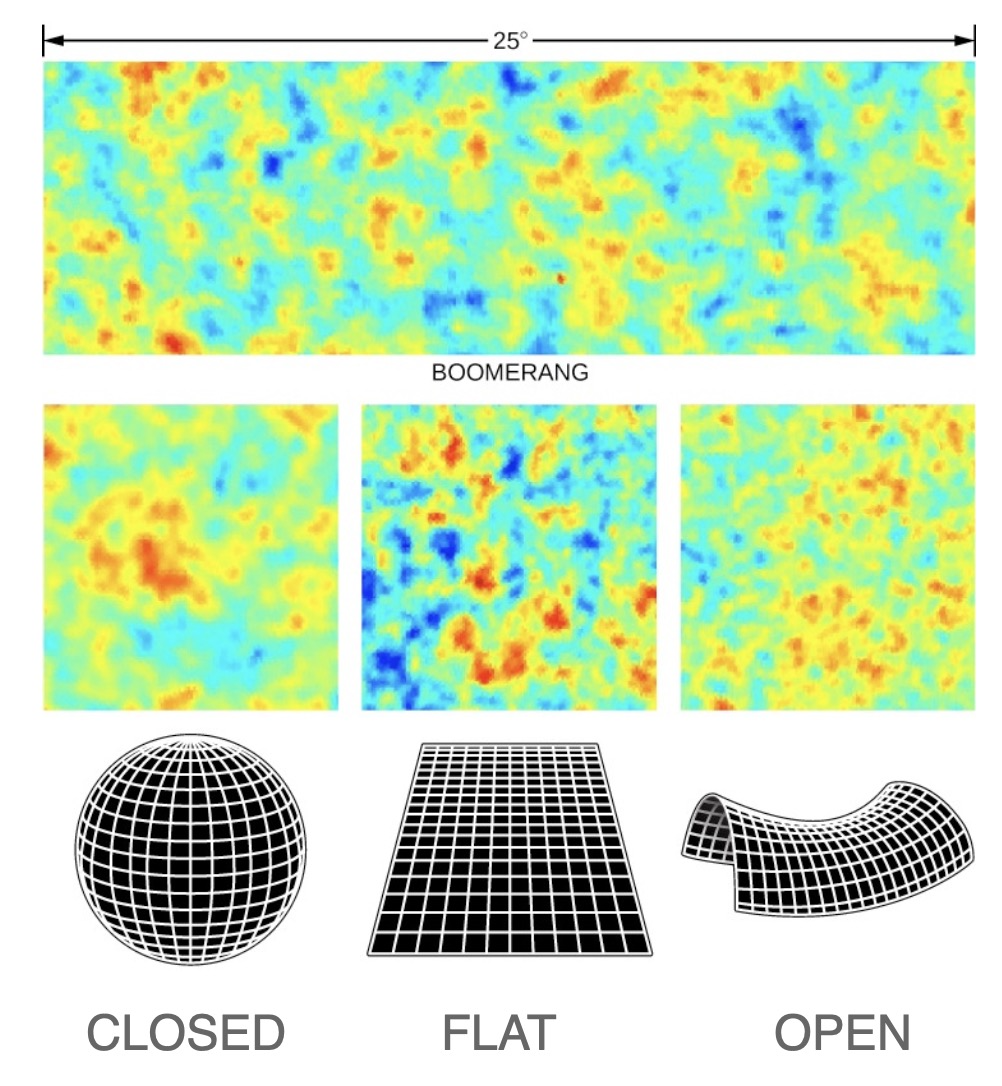
\includegraphics[width=0.6\columnwidth]{figures/cmb_curvature.png}
\caption{The effect of spatial curvature on the apparent angular size of features in the CMB. In a closed universe, features appear larger; in an open universe, smaller. CMB observations strongly favour a flat geometry ($\Omtot \approx 1$).}
\label{fig:cmb_geometry}
\end{figure}

\subsection*{The Integrated Sachs--Wolfe Effect}

The \textbf{integrated Sachs--Wolfe (ISW) effect} provides a direct probe of dark energy through the CMB. The physical mechanism is as follows. As a CMB photon falls into a gravitational potential well (such as that associated with a supercluster), it gains energy (is blueshifted). While the photon traverses the structure, the Universe continues to expand, and if dark energy is present and causing the expansion to accelerate, the potential well decays during the photon's passage. When the photon climbs back out, the potential is shallower than when it fell in, so the photon loses less energy climbing out than it gained falling in. The result is a net energy gain---a small temperature increase on the CMB in the direction of the supercluster. The reverse occurs for voids: photons crossing an underdensity experience a net energy loss.

Observationally, this is detected by cross-correlating the positions of large-scale structures (superclusters and voids) identified in galaxy surveys with the CMB temperature map. The detection of a positive correlation---hotter CMB in the direction of overdensities and cooler CMB toward voids---provides evidence for the decay of gravitational potentials, which in a matter-dominated universe would not occur. The ISW effect is therefore a signature of dark energy or, more generally, of any departure from matter domination at late times.

\begin{figure}[H]
\centering
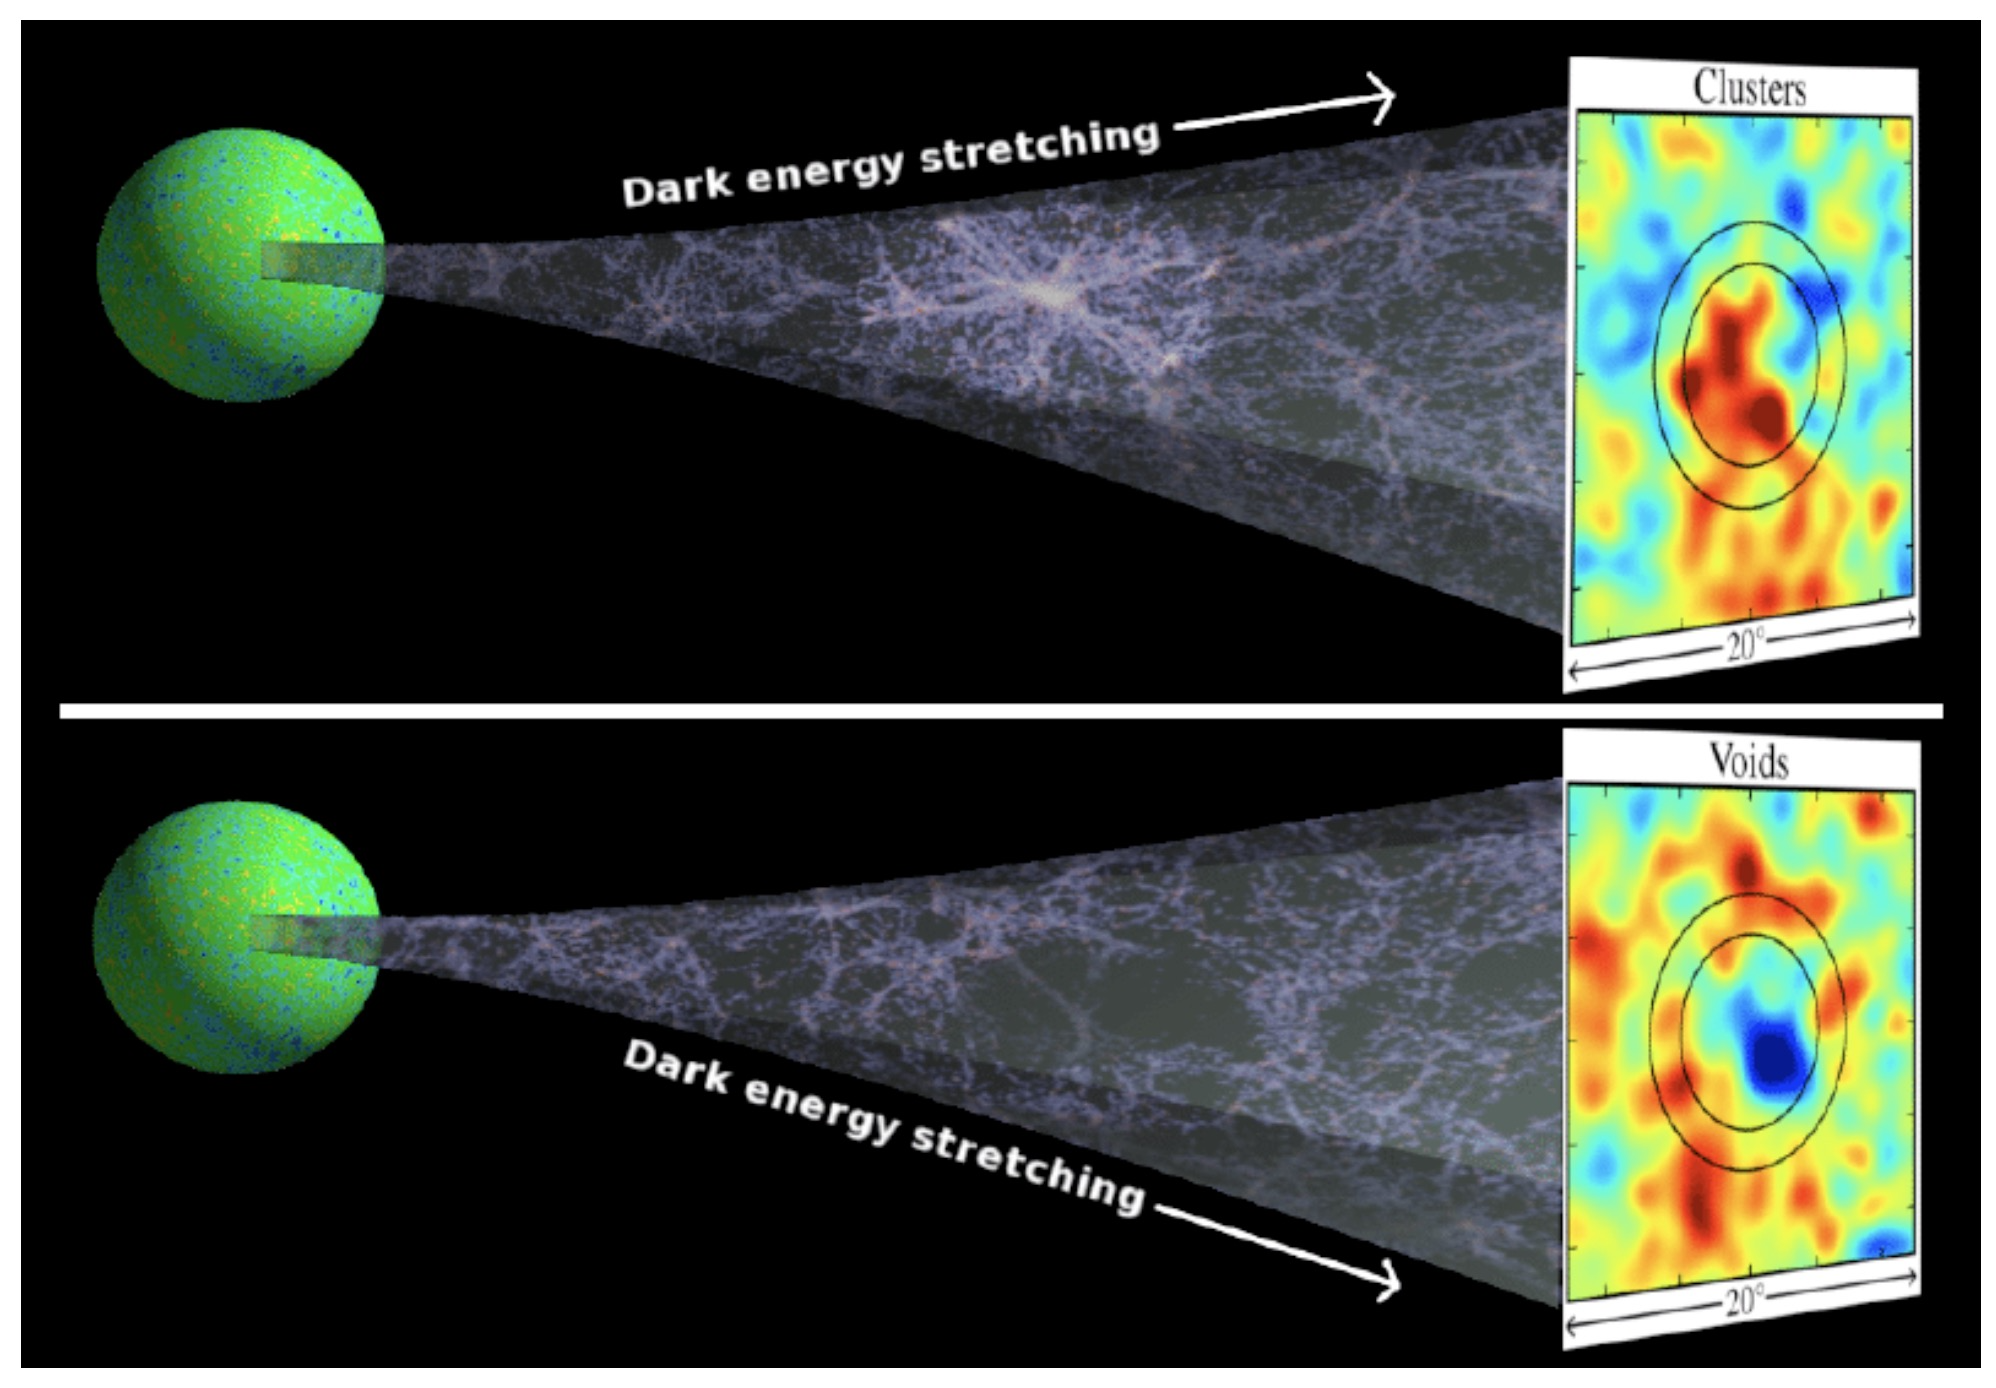
\includegraphics[width=0.7\columnwidth]{figures/sachs_wolfe.png}
\caption{Schematic illustration of the integrated Sachs--Wolfe (ISW) effect. A photon falling into a gravitational potential well gains energy. During transit, the accelerating expansion stretches the potential, so the photon loses less energy climbing out than it gained falling in. The net effect is a slight temperature increase toward superclusters and a decrease toward voids.}
\label{fig:isw_effect}
\end{figure}

\subsection*{Baryon Acoustic Oscillations}

Baryon acoustic oscillations (BAO) provide a powerful geometric probe of the expansion history. The BAO signal---a characteristic excess of galaxy pairs separated by approximately $150\,\mathrm{Mpc}$---acts as a standard ruler that can be measured at different redshifts to constrain both the angular diameter distance $D_A(z)$ and the Hubble parameter $H(z)$.

Combined BAO measurements from SDSS, BOSS, and eBOSS yield a detection of dark energy at greater than $8\sigma$ significance from BAO data alone, independent of any supernova or CMB data. When combined with CMB constraints and the supernova Hubble diagram, the BAO measurements provide some of the tightest constraints on the dark energy equation of state (see Chapter~\ref{ch:bao}).

\begin{figure}[H]
\centering
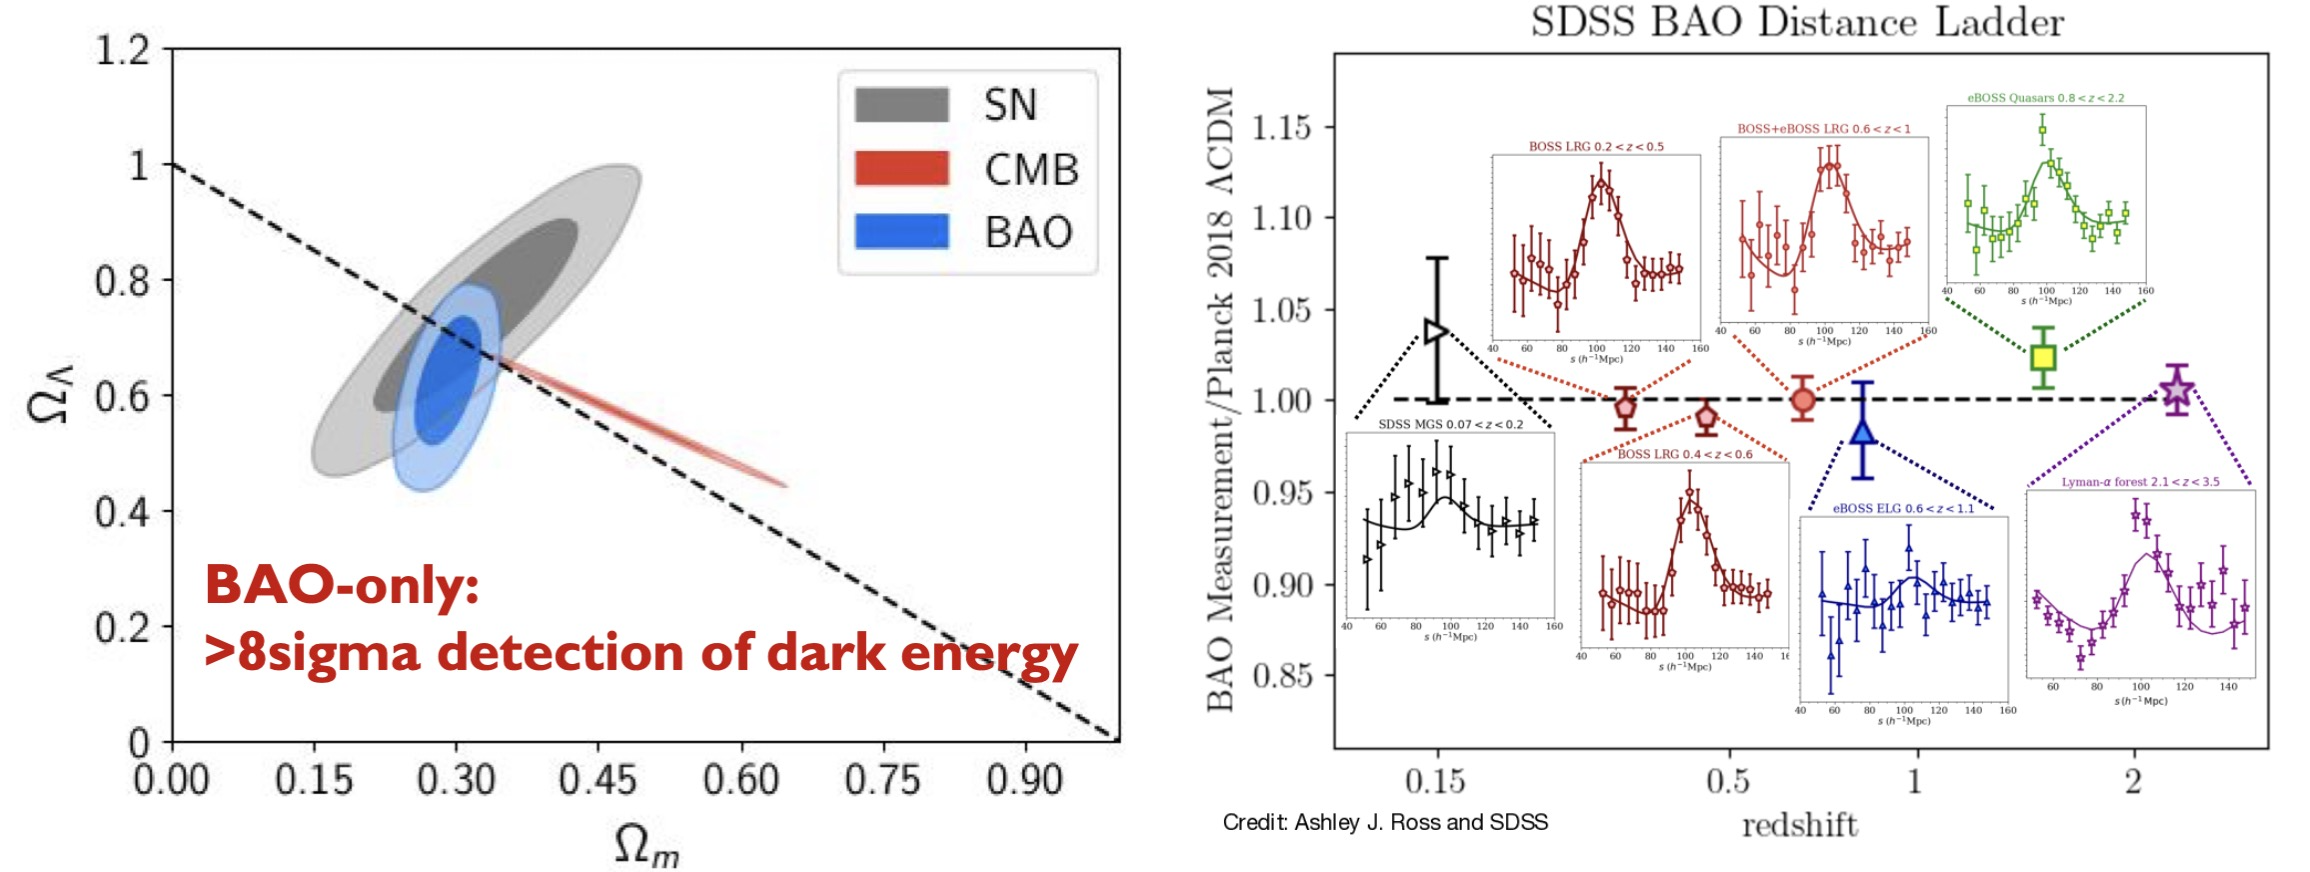
\includegraphics[width=0.7\columnwidth]{figures/bao_DE.png}
\caption{Constraints on the dark energy density from BAO measurements alone (SDSS/BOSS/eBOSS), demonstrating a detection of dark energy at greater than $8\sigma$ significance, independent of supernova or CMB data.}
\label{fig:bao_constraints}
\end{figure}


% ===================================================================
\section{The Cosmic Energy Budget}
\label{sec:energy_budget}
% ===================================================================

Combining all the observational probes described above---CMB, galaxy clustering, supernovae, gravitational lensing---gives us a remarkably consistent picture of the composition of the Universe:
\begin{itemize}
    \item \textbf{Ordinary (baryonic) matter}: approximately 5\% of the total energy density. This includes all atoms, stars, planets, gas, and dust.
    \item \textbf{Dark matter}: approximately 25\%. A non-luminous, non-baryonic component that interacts gravitationally but not electromagnetically.
    \item \textbf{Dark energy}: approximately 70\%. A component with negative pressure driving the accelerated expansion of the Universe.
\end{itemize}
Taken together, approximately 95\% of the energy content of the Universe is in forms that are not described by the Standard Model of particle physics. This is both humbling and exciting: the Universe is largely composed of substances whose fundamental nature remains unknown.

\begin{figure}[H]
\centering
% TODO: Add figure --- Cosmic energy budget pie chart
%\fbox{\parbox{0.8\textwidth}{\centering\vspace{2cm}\textit{Figure placeholder: Pie chart of the cosmic energy budget (5\% baryons, 25\% dark matter, 70\% dark energy)}\vspace{2cm}}}
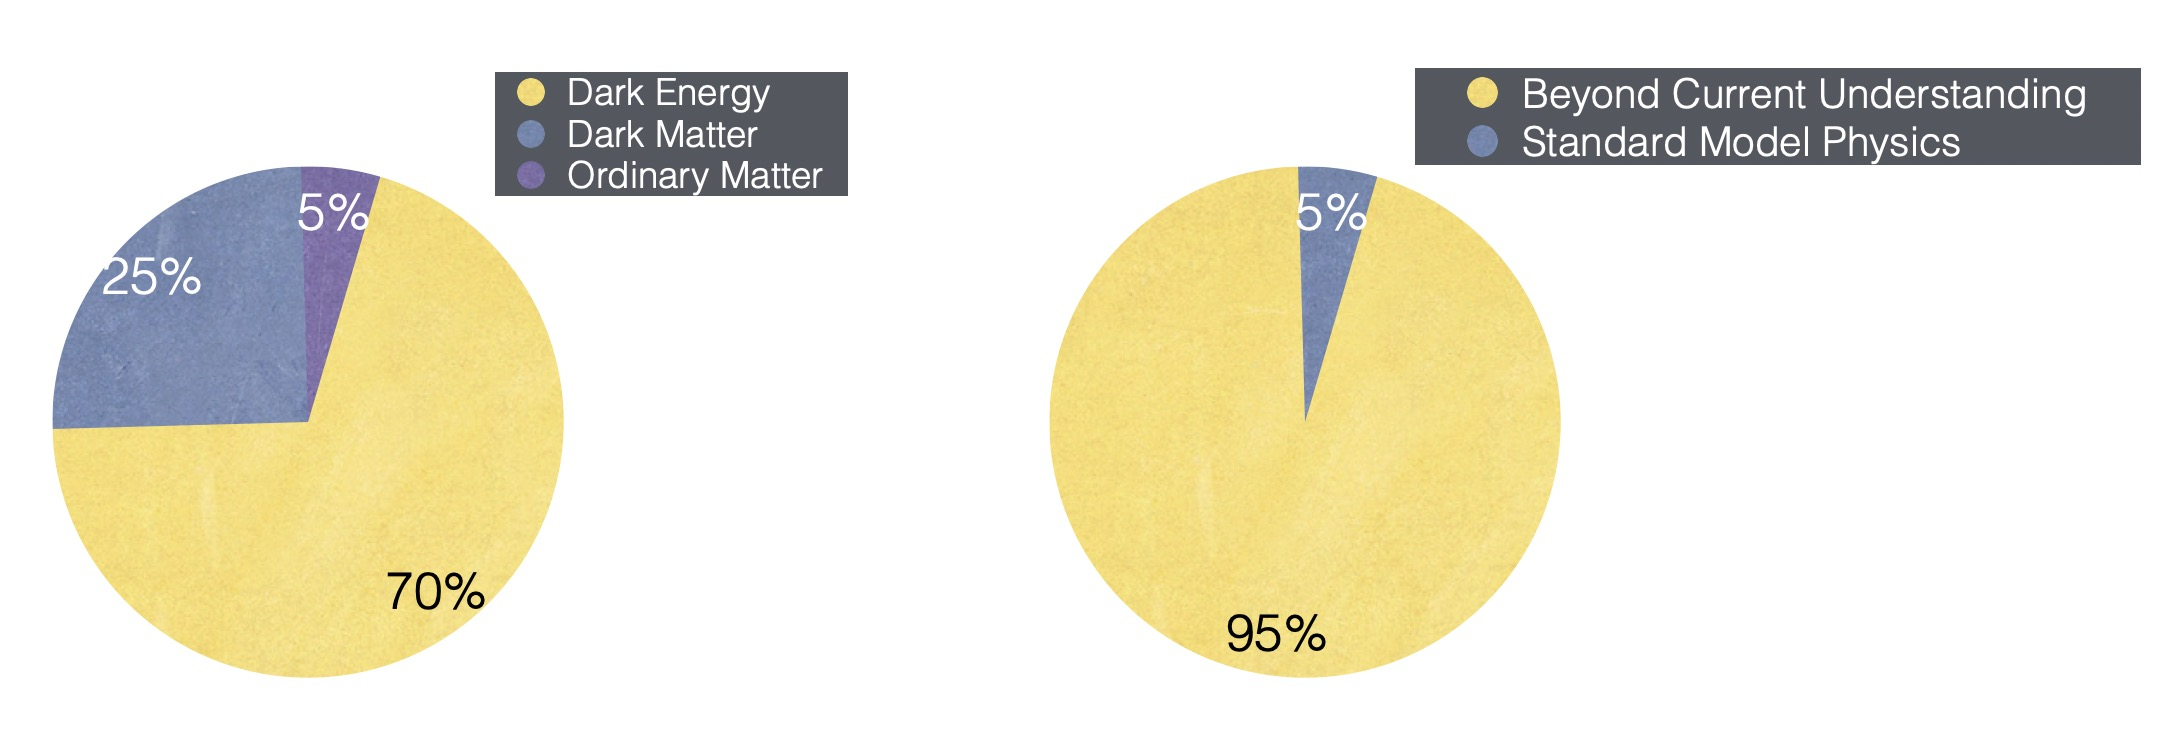
\includegraphics[width=\columnwidth]{figures/cosmic_pie.png}
\caption{The cosmic energy budget. Ordinary baryonic matter accounts for only about 5\% of the total energy density. Dark matter contributes roughly 25\%, and dark energy roughly 70\%. Approximately 95\% of the Universe is in forms not described by the Standard Model of particle physics.}
\label{fig:energy_budget}
\end{figure}


% ===================================================================
\section{Open Questions and Current Controversies}
\label{sec:open_questions}
% ===================================================================

The $\Lcdm$ model---a spatially flat universe with a cosmological constant ($\Lambda$) plus cold dark matter (CDM), described by just six free parameters---fits an impressive range of cosmological data: the CMB power spectrum, BAO, SNe Ia, gravitational lensing, and galaxy cluster counts. With only six numbers, plus some well-motivated assumptions, we can account for observations spanning 13.8 billion years of cosmic history. This is a remarkable achievement. However, several open questions and emerging tensions suggest that our understanding may be incomplete.

\subsection*{What is Dark Matter?}

The nature of dark matter remains one of the greatest unsolved problems in physics. A wide range of candidates have been proposed:
\begin{itemize}
    \item \textbf{Weakly Interacting Massive Particles (WIMPs)}: Motivated by supersymmetry and other beyond-Standard-Model theories. Extensive direct detection experiments have so far yielded null results, placing increasingly stringent limits on the WIMP--nucleon cross section.
    \item \textbf{Axions and axion-like particles}: Light bosonic particles originally proposed to solve the strong CP problem in quantum chromodynamics. Dedicated experiments such as ADMX are searching for axion signals.
    \item \textbf{Sterile neutrinos}: Hypothetical right-handed neutrinos that could serve as warm dark matter candidates.
    \item \textbf{Primordial black holes (PBHs)}: Black holes formed in the early Universe, potentially in a mass range not yet excluded by observations.
    \item \textbf{MACHOs} (Massive Compact Halo Objects): Baryonic objects such as brown dwarfs or black holes. Microlensing surveys have largely ruled out MACHOs as the dominant component of dark matter.
    \item \textbf{Modified gravity}: Alternatives such as Modified Newtonian Dynamics (MOND), Tensor--Vector--Scalar gravity (TeVeS), and entropic gravity attempt to explain dark matter phenomenology by modifying the law of gravity rather than introducing new particles. These models face significant challenges in explaining the full range of cosmological observations.
\end{itemize}

%\begin{figure}[H]
%\centering
% TODO: Add figure --- Dark matter candidates taxonomy
%\fbox{\parbox{0.8\textwidth}{\centering\vspace{2cm}\textit{Figure placeholder: Taxonomy of dark matter candidates}\vspace{2cm}}}
%\caption{A taxonomy of dark matter candidates, ranging from ultralight axions to primordial black holes, alongside modified gravity alternatives. The viable parameter space is being progressively constrained by direct detection, indirect detection, and collider experiments.}
%\label{fig:dm_candidates}
%\end{figure}

\subsection*{Reionisation and the Cosmic Dawn}

After recombination at $z\approx 1100$, the Universe entered the ``dark ages''---a period during which neutral hydrogen filled intergalactic space and no luminous sources existed. The formation of the first stars and galaxies at $z\sim 20$--$30$ began the process of \textbf{reionisation}, in which ultraviolet radiation from these first objects gradually ionised the intergalactic medium. The timing and topology of reionisation remain poorly constrained and are the subject of intensive observational efforts.

A particularly intriguing result came from the EDGES experiment, which in 2018 reported a detection of the global 21\,cm absorption signal from neutral hydrogen at $z\approx 17$, corresponding to the epoch when the first stars began illuminating the Universe. The absorption trough was deeper than expected, which, if confirmed, could point to exotic physics such as interactions between baryons and dark matter that cool the gas below the standard prediction.

\subsection*{The Hubble Tension}

Perhaps the most discussed discrepancy in modern cosmology is the \textbf{Hubble tension}: a persistent disagreement between two routes to measuring the present-day expansion rate~$\Hnot$.
\begin{itemize}
    \item \textbf{Early-universe route}: The Planck satellite's measurement of the CMB power spectrum, interpreted within the $\Lcdm$ model, yields $\Hnot = 67.4 \pm 0.5\kmsMpc$.
    \item \textbf{Late-universe route}: The SH0ES collaboration's calibration of the distance ladder using Cepheid variables and Type~Ia supernovae gives $\Hnot = 73.0 \pm 1.0\kmsMpc$.
\end{itemize}
The discrepancy is approximately $5\sigma$---far too large to be a statistical fluke. These two methods are measuring the same physical quantity; either one (or both) harbours an unidentified systematic error, or the $\Lcdm$ model is incomplete and new physics is required to reconcile them.

\begin{figure}[H]
\centering
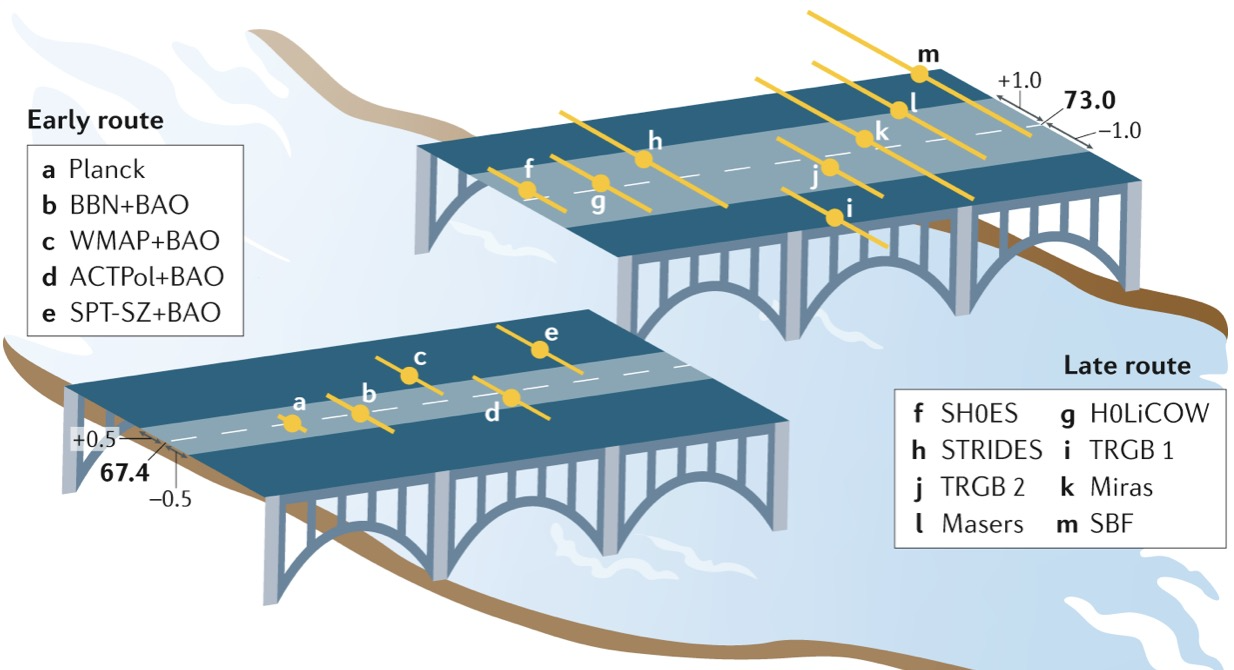
\includegraphics[width=0.8\columnwidth]{figures/H0_early_late.png}
\caption{Summary of $\Hnot$ measurements. Early-universe determinations (CMB, BAO) cluster around $67$--$68\kmsMpc$, while late-universe determinations (Cepheids, SNe~Ia, strong lensing time delays) cluster around $72$--$74\kmsMpc$. The $\sim 5\sigma$ discrepancy is the Hubble tension.}
\label{fig:hubble_tension}
\end{figure}

\subsection*{Evolving Dark Energy?}

The simplest model for dark energy is a cosmological constant~$\Lambda$ with a constant equation of state $w = -1$. However, recent results from the DESI collaboration, combining BAO measurements with various supernova samples, show hints of tension with this simple picture. When the dark energy equation of state is allowed to vary with time using the CPL parametrisation $w(a) = w_0 + w_a(1-a)$, the data show a preference for $w_0 > -1$ and $w_a < 0$---that is, dark energy that was less negative in the past and has become more negative over time. When CMB constraints from Planck are added, the preference for time-varying dark energy strengthens.

These results are tantalising but not yet conclusive. Systematic effects in the supernova samples---including a potential correlation between supernova peak brightness and the age of the host galaxy's stellar population---are being actively investigated. Future DESI data releases, combined with next-generation supernova surveys, will clarify whether dark energy truly evolves.

\begin{figure}[H]
\centering
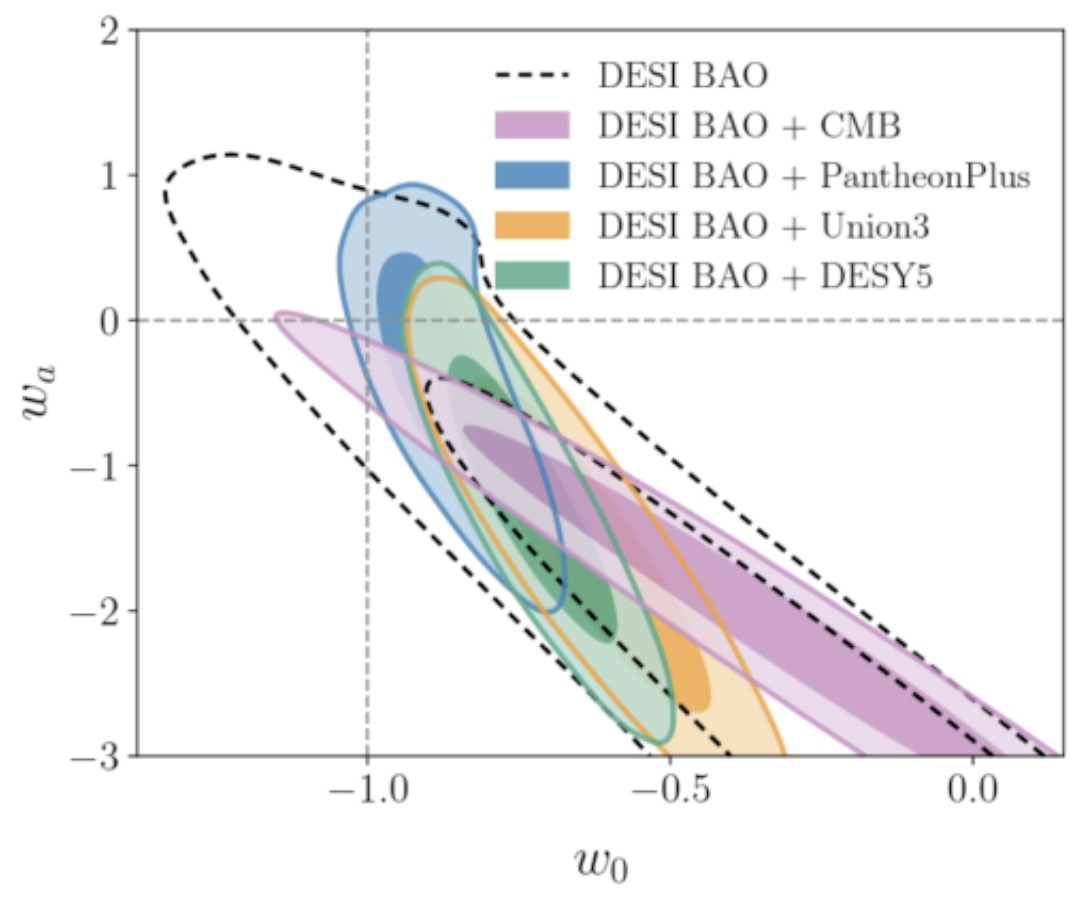
\includegraphics[width=0.7\columnwidth]{figures/w0_bao_sne.png}
\caption{Constraints on the dark energy equation of state parameters $w_0$ and $w_a$ from DESI BAO data combined with various supernova samples and Planck CMB data. The cosmological constant ($w_0=-1$, $w_a=0$) lies at the edge of the allowed region, suggesting possible time evolution of dark energy.}
\label{fig:desi_de}
\end{figure}

\subsection*{The $\sigmaEight$ Tension}

A second, less dramatic but persistent, discrepancy has emerged in the amplitude of matter density fluctuations, characterised by the parameter $\sigmaEight$ (the root-mean-square fluctuation in spheres of radius $8\,h^{-1}\,\mathrm{Mpc}$). The value inferred from the CMB (assuming $\Lcdm$) is somewhat higher than that measured directly from weak gravitational lensing surveys at lower redshift. Although the significance is currently $2$--$3\sigma$---less alarming than the Hubble tension---it may point to the same underlying issue: either unaccounted-for systematics or a departure from $\Lcdm$.

%\begin{figure}[H]
%\centering
% TODO: Add figure --- sigma_8 tension plot
%\fbox{\parbox{0.8\textwidth}{\centering\vspace{2cm}\textit{Figure placeholder: $\sigmaEight$ measurements from CMB vs.\ weak lensing surveys}\vspace{2cm}}}
%\caption{Comparison of $\sigmaEight$ (or the related quantity $S_8 = \sigmaEight\sqrt{\Omm/0.3}$) as measured from the CMB (Planck) and from weak lensing surveys (KiDS, DES, HSC). The CMB-inferred value is consistently higher than the direct low-redshift measurements.}
%\label{fig:sigma8_tension}
%\end{figure}

\subsection{Paradigm Shifts in Cosmology}

The philosopher of science Thomas Kuhn, in \textit{The Structure of Scientific Revolutions}, proposed a model in which science alternates between periods of ``normal science'' (incremental progress within an accepted paradigm) and ``revolutionary science'' (paradigm shifts triggered by the accumulation of anomalies). The $\Lcdm$ model has been the reigning paradigm for over two decades. The emerging tensions described above---if they survive further scrutiny---may represent the first cracks that herald a new paradigm shift in our understanding of the cosmos.


% ===================================================================
\section{Looking Ahead}
\label{sec:looking_ahead}
% ===================================================================

The coming decade promises to be an exceptionally exciting time for cosmology. New surveys and instruments will vastly expand our observational reach:
\begin{itemize}
    \item \textbf{Spectroscopic surveys}: DESI is only the beginning. Future instruments such as K-Spec are being planned to map faint galaxies at high redshift, opening new windows into the growth of large-scale structure.
    \item \textbf{New imaging}: Missions like Euclid (ESA) and the Vera C.\ Rubin Observatory (formerly LSST) will provide deep, wide-field imaging for weak lensing, galaxy clustering, and photometric redshift measurements. A proposed Korean mission, S-DRIFT, aims to map low surface brightness galaxies, informing our understanding of galaxy evolution, dark matter, and potentially even gravity.
    \item \textbf{Radio astronomy and 21\,cm cosmology}: Next-generation radio telescopes will map neutral hydrogen through the epoch of reionisation and into the dark ages, probing the Universe at redshifts inaccessible to optical surveys.
    \item \textbf{Gravitational wave astronomy}: Space-based detectors such as LISA will enable entirely new tests of cosmology, from measuring the Hubble constant via ``standard sirens'' to probing the nature of dark energy through the gravitational wave background.
\end{itemize}

Whether these observations confirm the $\Lcdm$ model with ever greater precision or reveal fundamental departures from it, the era of precision cosmology is far from over.

\bigskip
\noindent\textbf{In the next lecture} we will develop the mathematical framework for the expanding universe: the Friedmann--Lema\^{i}tre--Robertson--Walker (FLRW) metric, the Friedmann equations governing the scale factor $a(t)$, the energy components driving expansion, and the definition of cosmological distances.


% --- Lecture 2 ----------------------------------------------------------
\chapter{Expanding Universe and Background Dynamics}
\label{ch:background_dynamics}

In this chapter we will look at the expansion and background dynamics of the Universe on large scales. Firstly, we will employ the use of General Relativity, which will require us to consider several crucial concepts such as the metric and the energy-momentum tensor in our journey towards a description of the expansion dynamics. However, later in this chapter, we will show that the same equations can, in fact, be obtained from a much simpler Newtonian derivation. With the so-called Friedmann Equations in hand we proceed to solve them in various scenarios, and we will see what this means for the expansion of the Universe and its ultimate fate. 


\section*{Interlude: A Brief Review of Tensor Algebra}

This is not a course in General Relativity. We do not have the time to explain the theory in detail. However, if you have studied GR before it may still be useful for a refresher on index notation and tensor operations that we will use throughout.

\subsection*{Index notation and the Einstein summation convention}

In general relativity, quantities carry \emph{indices} that label their components. Greek indices ($\mu, \nu, \lambda, \ldots$) run over all four spacetime dimensions: $0,1,2,3$ (time and three spatial directions). Latin indices ($i, j, k, \ldots$) run over only the three spatial dimensions: $1,2,3$.

The \textbf{Einstein summation convention} states that whenever an index appears once as a superscript (upper) and once as a subscript (lower) in the same term, a sum over all values of that index is implied:
\begin{equation}
    A^\mu B_\mu \equiv \sum_{\mu=0}^{3} A^\mu B_\mu = A^0 B_0 + A^1 B_1 + A^2 B_2 + A^3 B_3\,.
\end{equation}
Such a repeated index is called a \emph{dummy} or \emph{contracted} index. An index that appears only once (and is not summed over) is called a \emph{free} index.

\subsection*{The metric tensor and raising/lowering indices}

The metric tensor $g_{\mu\nu}$ is the central object that defines the geometry of spacetime. It determines the invariant interval (``distance'') between nearby events:
\begin{equation}
    ds^2 = g_{\mu\nu}\,dx^\mu\,dx^\nu\,.
\end{equation}
The metric is symmetric: $g_{\mu\nu}=g_{\nu\mu}$.

Its inverse, denoted $g^{\mu\nu}$, is defined by the condition
\begin{equation}
    g^{\mu\alpha}\,g_{\alpha\nu} = \delta^\mu_{\ \nu}\,,
\end{equation}
where $\delta^\mu_{\ \nu}$ is the \textbf{Kronecker delta}: $\delta^\mu_{\ \nu}=1$ if $\mu=\nu$ and $0$ otherwise. The trace of the Kronecker delta gives the dimension of the space: $\delta^\mu_{\ \mu}=4$ in four-dimensional spacetime, or $\delta^i_{\ i}=3$ for the spatial part.

The metric and its inverse allow us to \textbf{raise and lower indices}, converting between contravariant (upper) and covariant (lower) components of a tensor:
\begin{align}
    \text{Lowering:} &\qquad V_\mu = g_{\mu\nu}\,V^\nu\,,\\[4pt]
    \text{Raising:}  &\qquad V^\mu = g^{\mu\nu}\,V_\nu\,.
\end{align}
For a tensor with multiple indices, each index is raised or lowered independently. For example:
\begin{equation}
    T^{\mu}_{\ \nu} = g^{\mu\alpha}\,T_{\alpha\nu}\,,\qquad T^{\mu\nu} = g^{\mu\alpha}\,g^{\nu\beta}\,T_{\alpha\beta}\,.
\end{equation}
Physically, $V^\mu$ and $V_\mu$ represent the same geometric object (a vector) expressed in two different ways. The metric converts between them, accounting for the curvature of the space.

\subsection*{Contraction}

\textbf{Contraction} means setting an upper and a lower index equal and summing (i.e.\ taking a trace). For example, from a rank-2 tensor $T^{\mu}_{\ \nu}$, the contraction $T^\mu_{\ \mu}$ produces a scalar (a single number at each point). A familiar example is the Ricci scalar, obtained by contracting the Ricci tensor:
\begin{equation}
    R = g^{\mu\nu}\,R_{\mu\nu}\,.
\end{equation}
Here the metric first raises one index of $R_{\mu\nu}$ and then the contraction is taken, but the two operations are combined in one step.

\medskip
These conventions are all we need to follow the GR derivation of the Friedmann equations that follows.


\section{Friedmann via General Relativity }

\subsection{The Metric, $g_{\mu \nu}$}
A metric is the object that tells you how to compute distances (and time intervals) in a given spacetime. More precisely, it defines the infinitesimal interval $ds^{2}$ between two neighbouring events as a function of the coordinate differentials. Once you have the metric, you have the geometry---you can compute distances, angles, volumes, geodesics (the paths of freely falling particles and light rays), and ultimately the curvature of spacetime itself.

Students will already be familiar with one metric: the Minkowski metric of special relativity,
\begin{equation}
    ds^{2} = -c^{2}\,dt^{2} + dx^{2} + dy^{2} + dz^{2},
    \label{eq:minkowski}
\end{equation}
which describes a flat, static spacetime with no gravity. The minus sign in front of the time component is what distinguishes spacetime geometry from ordinary Euclidean geometry---it encodes the fact that time and space are not equivalent, and it gives rise to the causal structure of light cones. Intervals with $ds^{2}<0$ are timelike (traversable by massive particles), $ds^{2}=0$ are null (traversed by light), and $ds^{2}>0$ are spacelike (no causal connection).

The key point is that the Minkowski metric has constant coefficients---nothing depends on position or time. This reflects the fact that special relativity describes a spacetime with no gravity and no expansion. General relativity generalises this by allowing the coefficients in front of the coordinate differentials to become functions of the coordinates. In the most general case one writes
\begin{equation}
    ds^{2} = g_{\mu\nu}\,dx^{\mu}\,dx^{\nu},
    \label{eq:general_metric}
\end{equation}
where $g_{\mu\nu}$ is a symmetric $4\times 4$ matrix (the metric tensor) that can vary from point to point. For Minkowski spacetime, $g_{\mu\nu} = \eta_{\mu\nu} = \mathrm{diag}(-c^{2},\,1,\,1,\,1)$ everywhere. For the Schwarzschild solution around a spherical mass, the coefficients depend on the radial coordinate~$r$. For cosmology, the FLRW metric has coefficients that depend on time through the scale factor $a(t)$---this single function encodes the entire expansion history of the universe.

So when we write down the FLRW metric, we are specifying the geometry of a universe that is spatially homogeneous and isotropic but whose spatial distances are stretching (or contracting) with time. Everything else---the Friedmann equations, the Hubble law, the redshift, the horizon structure---follows from this one object.


\subsection{Friedmann--Lema\^{i}tre--Robertson--Walker (FLRW) metric }
The Friedmann--Lema\^{i}tre--Robertson--Walker (FLRW) metric is the exact solution to Einstein's field equations that describes a homogeneous, isotropic, expanding (or contracting) universe. It is the mathematical backbone of modern physical cosmology.

The FLRW metric is, in essence, the \emph{unique} metric (up to a choice of spatial curvature) that follows from imposing the \textbf{cosmological principle}: the assumption that the universe is spatially homogeneous and isotropic on sufficiently large scales. Homogeneity means no preferred location; isotropy means no preferred direction. Together these drastically constrain the geometry---the spatial part of the metric must be a maximally symmetric 3-space, leaving only three possibilities for spatial curvature (positive, zero, or negative), plus a single free function of time, the scale factor $a(t)$.

The logical chain is therefore:
\begin{equation*}
    \text{Einstein's Field Equations} + \text{Cosmological Principle} \;\Longrightarrow\; \text{FLRW Metric.}
\end{equation*}

Observational support comes from the large-scale galaxy distribution, the near-perfect isotropy of the CMB (with $\delta T/T \sim 10^{-5}$), and the isotropic Hubble flow. The principle is, of course, an approximation---it holds statistically on scales $\gtrsim 100\,h^{-1}\,\mathrm{Mpc}$, while structure on smaller scales (clusters, filaments, voids) is treated as perturbations on top of the FLRW background.

\subsection{Historical Development}

The metric carries four names because it was assembled in stages over roughly two decades.

\subsection*{Alexander Friedmann (1922, 1924)}

Friedmann derived the first dynamical cosmological solutions to Einstein's equations, showing that the universe need not be static. His 1922 paper treated the positive-curvature case and his 1924 paper the negative-curvature case. Einstein initially thought there was a mathematical error, later retracted the objection, but never took the physical implications seriously during Friedmann's lifetime. Friedmann died in 1925.

\subsection*{Georges Lema\^{i}tre (1927)}

Lema\^{i}tre independently derived an expanding solution, and---crucially---connected it to observational data, proposing a linear relation between recession velocity and distance (what we now call the Hubble law, two years before Hubble's 1929 paper). His paper, published in French in an obscure Belgian journal, went essentially unnoticed until Eddington drew attention to it in 1931.

There is a notable historical injustice in the naming. Lema\^{i}tre's contribution was under-recognized for decades, partly due to a mistranslation of his 1927 paper into English in 1931 where the key paragraphs establishing the velocity--distance relation were omitted. Only in 2011 did Mario Livio show this was likely Lema\^{i}tre's own editorial decision, though the broader neglect of his priority remains a sore point in the history of cosmology.

\subsection*{Howard Percy Robertson (1935, 1936) and Arthur Geoffrey Walker (1937)}

Robertson and Walker independently gave a rigorous differential-geometric proof that homogeneity and isotropy \emph{uniquely} determine the metric form (up to the curvature parameter and scale factor). Their contribution was less about finding solutions to Einstein's equations and more about proving a geometric theorem: the most general metric consistent with the cosmological principle must take the form we now write down. This is why the metric is sometimes called simply the ``Robertson--Walker'' metric when one wishes to emphasize the kinematic/geometric content without reference to the dynamics.

\subsection{The Line Element}

In comoving coordinates $(t,\, r,\, \theta,\, \phi)$ with signature $(-,+,+,+)$, the FLRW metric is:
\begin{equation}
    \boxed{\;
    ds^{2} = -c^{2}\,dt^{2}
    + a^{2}(t)\!\left[\frac{dr^{2}}{1-kr^{2}}
    + r^{2}\!\left(d\theta^{2} + \sin^{2}\!\theta\;d\phi^{2}\right)\right]
    \;}
    \label{eq:flrw}
\end{equation}
where:
\begin{itemize}
    \item $t$ is \textbf{cosmic time}, the proper time measured by comoving observers (those at rest with respect to the Hubble flow).
    \item $a(t)$ is the \textbf{scale factor}, encoding the expansion history. It is conventionally normalised to $a(t_{0})=1$ today.
    \item $k$ is the \textbf{curvature parameter}: $k=+1$ (closed, spherical), $k=0$ (flat, Euclidean), or $k=-1$ (open, hyperbolic). Some conventions absorb a length scale into $k$ so that it can take any real value, but the sign is what matters physically.
    \item $r$ is a dimensionless \textbf{comoving radial coordinate}; physical distance is $a(t)\cdot r$.
\end{itemize}

Reading off the metric components from Eq.~\eqref{eq:flrw}, the non-zero components are
\begin{equation}
    g_{00} = -c^2,\qquad g_{rr} = \frac{a^2}{1-kr^2},\qquad g_{\theta\theta} = a^2 r^2,\qquad g_{\phi\phi} = a^2 r^2\sin^2\!\theta,
\end{equation}
with inverses obtained from $g^{\mu\alpha}g_{\alpha\nu}=\delta^\mu_{\ \nu}$:
\begin{equation}
    g^{00} = -\frac{1}{c^2},\qquad g^{rr} = \frac{1-kr^2}{a^2},\qquad g^{\theta\theta} = \frac{1}{a^2 r^2},\qquad g^{\phi\phi} = \frac{1}{a^2 r^2\sin^2\!\theta}\,.
\end{equation}

\medskip
\noindent\textbf{Convention:} From here on, we adopt \textbf{natural units} $c=1$ for the GR derivation. In these units $g_{00}=-1$ and the metric~\eqref{eq:flrw} becomes $ds^2=-dt^2+a^2(t)[\cdots]$. This keeps the algebra clean and is standard in GR treatments. We will restore explicit factors of $c$ where needed (e.g.\ in the energy--momentum tensor and the continuity equation).

\subsection{Christoffel Symbols}

The Christoffel symbols (or Levi-Civita connection coefficients) encode how the coordinate basis vectors change from point to point in curved spacetime. They are defined entirely in terms of the metric and its first derivatives:
\begin{equation}
    \Gamma^\mu_{\alpha\beta} = \frac{1}{2}\,g^{\mu\nu}\bigl(\partial_\alpha g_{\nu\beta} + \partial_\beta g_{\nu\alpha} - \partial_\nu g_{\alpha\beta}\bigr).
\end{equation}
Since the metric is diagonal, the computation simplifies considerably. In our $c=1$ units, $g_{00}=-1$ is constant, $g_{0i}=0$, and the spatial components $g_{ij}$ depend on both time (through $a(t)$) and the spatial coordinates (through the curvature terms). We organize the non-vanishing components into three groups.

\subsection*{Mixed temporal--spatial: $\Gamma^0_{ij}$}

These components arise because the spatial metric changes with time (the Universe expands or contracts). Setting $\mu=0$, only the $\nu=0$ term in the sum survives (since $g^{0\nu}$ is non-zero only for $\nu=0$, as the metric is diagonal). The only non-zero contribution comes from $-\partial_0 g_{ij}$:
\begin{align}
    \Gamma^0_{rr} &= \frac{a\dot{a}}{1-kr^2}\,,\\[4pt]
    \Gamma^0_{\theta\theta} &= a\dot{a}\,r^2\,,\\[4pt]
    \Gamma^0_{\phi\phi} &= a\dot{a}\,r^2\sin^2\!\theta\,.
\end{align}
Comparing with the metric components, these can be written compactly as
\begin{equation}\label{eq:gamma0ij}
    \Gamma^0_{ij} = \frac{\dot{a}}{a}\,g_{ij} = H\,g_{ij}\,,
\end{equation}
where $H\equiv\dot{a}/a$ is the Hubble parameter. This compact form will greatly simplify the calculation of the Ricci tensor.

\subsection*{Mixed temporal--spatial: $\Gamma^i_{0j}$}

These components describe how the spatial basis vectors are ``stretched'' by the expansion. The calculation is the same as in the flat case because the $g^{ik}$ and $\partial_0 g_{kj}$ factors always combine to give a Kronecker delta:
\begin{equation}\label{eq:gammai0j}
    \Gamma^i_{0j} = \frac{1}{2}\,g^{ik}\,\partial_0 g_{kj} = \frac{1}{2}\,g^{ik}\cdot 2\dot{a}a\,\gamma_{kj} = \frac{\dot{a}}{a}\,\delta^i_{\ j} = H\,\delta^i_{\ j}\,,
\end{equation}
where $\gamma_{kj}$ is the time-independent part of the spatial metric ($g_{kj}=a^2\gamma_{kj}$). Explicitly: $\Gamma^r_{0r}=\Gamma^\theta_{0\theta}=\Gamma^\phi_{0\phi}=H$. Note that this result is independent of the spatial curvature $k$.

\subsection*{Purely spatial: $\Gamma^i_{jk}$}

Unlike the flat case in Cartesian coordinates, the spatial metric now has coordinate dependence through both the curvature term $1/(1-kr^2)$ and the standard spherical coordinate factors. These Christoffel symbols are those of the three-dimensional spatial geometry:

\medskip
\noindent\textbf{$r$-components:}
\begin{align}
    \Gamma^r_{rr} &= \frac{kr}{1-kr^2}\,,\\[4pt]
    \Gamma^r_{\theta\theta} &= -r(1-kr^2)\,,\\[4pt]
    \Gamma^r_{\phi\phi} &= -r(1-kr^2)\sin^2\!\theta\,.
\end{align}

\noindent\textbf{$\theta$-components:}
\begin{align}
    \Gamma^\theta_{r\theta} = \Gamma^\theta_{\theta r} &= \frac{1}{r}\,,\\[4pt]
    \Gamma^\theta_{\phi\phi} &= -\sin\theta\cos\theta\,.
\end{align}

\noindent\textbf{$\phi$-components:}
\begin{align}
    \Gamma^\phi_{r\phi} = \Gamma^\phi_{\phi r} &= \frac{1}{r}\,,\\[4pt]
    \Gamma^\phi_{\theta\phi} = \Gamma^\phi_{\phi\theta} &= \cot\theta\,.
\end{align}

Note that the $1/r$ and $\cot\theta$ terms are simply the standard spherical coordinate contributions and are present even when $k=0$. The genuinely curvature-dependent terms are those containing $k$ explicitly: $\Gamma^r_{rr}$ and the $(1-kr^2)$ factors in $\Gamma^r_{\theta\theta}$ and $\Gamma^r_{\phi\phi}$.

All other Christoffel symbols vanish ($\Gamma^0_{00}=\Gamma^0_{0i}=\Gamma^i_{00}=0$).

\subsection{The Ricci Tensor}

The Ricci tensor is constructed from the Christoffel symbols and their derivatives. Physically, it encodes how volumes of small balls of test particles are distorted by the curvature of spacetime. It is defined as a contraction of the Riemann curvature tensor $R^\lambda_{\ \mu\lambda\nu}$, which gives:
\begin{equation}\label{eq:ricci}
    R_{\mu\nu} = \partial_\lambda\Gamma^\lambda_{\mu\nu} - \partial_\nu\Gamma^\lambda_{\mu\lambda} + \Gamma^\lambda_{\lambda\sigma}\Gamma^\sigma_{\mu\nu} - \Gamma^\lambda_{\nu\sigma}\Gamma^\sigma_{\mu\lambda}\,.
\end{equation}
The first two terms involve derivatives of the Christoffel symbols, while the last two are quadratic in the Christoffel symbols. This structure means the Ricci tensor contains second derivatives of the metric, as expected for a quantity that describes curvature.

\subsection*{Strategy: Exploiting Symmetry}

By the isotropy and homogeneity of the FLRW metric, the Ricci tensor must take the form
\begin{equation}
    R_{0i} = 0\,,\qquad R_{ij} = f(t)\,g_{ij}\,,
\end{equation}
for some function $f(t)$. The vanishing of $R_{0i}$ follows from spatial isotropy: there is no preferred spatial direction. The proportionality of $R_{ij}$ to $g_{ij}$ follows from the fact that $g_{ij}$ is the only available symmetric spatial tensor. This means we only need to compute $R_{00}$ and determine the single function $f(t)$ to know the full Ricci tensor.

\subsection*{Computing $R_{00}$}

We evaluate each of the four terms in Eq.~\eqref{eq:ricci} with $\mu=\nu=0$, carefully tracking which Christoffel symbols contribute.

\medskip\noindent\textbf{Term 1:} $\partial_\lambda\Gamma^\lambda_{00}$.

This term requires Christoffel symbols with both lower indices equal to 0. Since $g_{00}=-1$ is constant and $g_{0i}=0$, we have $\Gamma^\lambda_{00}=0$ for all $\lambda$:
\begin{equation}
    \partial_\lambda\Gamma^\lambda_{00} = 0\,.
\end{equation}

\medskip\noindent\textbf{Term 2:} $-\partial_0\Gamma^\lambda_{0\lambda}$.

This is a trace over $\lambda$. For $\lambda=0$: $\Gamma^0_{00}=0$. For $\lambda=i$: $\Gamma^i_{0i}=H$. Since the spatial index runs over three dimensions:
\begin{equation}
    \Gamma^\lambda_{0\lambda} = 3H = 3\,\frac{\dot{a}}{a}\,.
\end{equation}
Taking the time derivative using the quotient rule $\partial_0(\dot{a}/a)=\ddot{a}/a-\dot{a}^2/a^2$:
\begin{equation}
    -\partial_0\!\left(3\,\frac{\dot{a}}{a}\right) = -3\left(\frac{\ddot{a}}{a} - \frac{\dot{a}^2}{a^2}\right) = -3\,\frac{\ddot{a}}{a} + 3H^2\,.
\end{equation}

\medskip\noindent\textbf{Term 3:} $\Gamma^\lambda_{\lambda\sigma}\Gamma^\sigma_{00}$.

This term vanishes because $\Gamma^\sigma_{00}=0$ for all $\sigma$, as argued above:
\begin{equation}
    \Gamma^\lambda_{\lambda\sigma}\Gamma^\sigma_{00} = 0\,.
\end{equation}

\medskip\noindent\textbf{Term 4:} $-\Gamma^\lambda_{0\sigma}\Gamma^\sigma_{0\lambda}$.

The non-zero $\Gamma$ symbols with a 0 in the lower slot are $\Gamma^i_{0j}=H\,\delta^i_{\ j}$. Therefore both $\lambda$ and $\sigma$ must be spatial:
\begin{equation}
    -\Gamma^i_{0j}\,\Gamma^j_{0i} = -H^2\,\delta^i_{\ j}\,\delta^j_{\ i} = -H^2\,\delta^i_{\ i}\,.
\end{equation}
The contraction $\delta^i_{\ j}\,\delta^j_{\ i}$ first collapses via the summed index $j$ into $\delta^i_{\ i}$, which is the trace of the $3\times 3$ identity matrix --- simply the number of spatial dimensions:
\begin{equation}
    \delta^i_{\ i} = \delta^1_{\ 1}+\delta^2_{\ 2}+\delta^3_{\ 3} = 3\,.
\end{equation}
Thus:
\begin{equation}
    -\Gamma^i_{0j}\,\Gamma^j_{0i} = -3H^2\,.
\end{equation}

\medskip\noindent\textbf{Combining all four terms:}
\begin{equation}
\boxed{R_{00} = 0 + \left(-3\,\frac{\ddot{a}}{a} + 3H^2\right) + 0 + \left(-3H^2\right) = -3\,\frac{\ddot{a}}{a}\,.}
\end{equation}
An important feature: $R_{00}$ is independent of the spatial curvature $k$. This is because the $00$ component only involves Christoffel symbols $\Gamma^i_{0j}$, which themselves are insensitive to $k$.

\subsection*{Computing $R_{ij}$}

The spatial components of the Ricci tensor are more involved because the purely spatial Christoffel symbols $\Gamma^i_{jk}$ now contribute. We use the compact forms $\Gamma^0_{ij}=Hg_{ij}$ and $\Gamma^i_{0j}=H\delta^i_{\ j}$ from Eqs.~\eqref{eq:gamma0ij}--\eqref{eq:gammai0j} to organize the calculation.

The key idea is to separate each term in Eq.~\eqref{eq:ricci} into contributions involving time (the Hubble parameter $H$) and those involving only the spatial geometry (the 3-dimensional Christoffel symbols). The spatial contributions will ultimately combine into the Ricci tensor of the constant-curvature 3-space.

\medskip\noindent\textbf{Term 1:} $\partial_\lambda\Gamma^\lambda_{ij}$.

We split the sum into $\lambda=0$ and $\lambda=k$:
\begin{equation}
    \partial_0\Gamma^0_{ij} + \partial_k\Gamma^k_{ij}\,.
\end{equation}
For the temporal part, using $\Gamma^0_{ij}=Hg_{ij}$ and $\dot{g}_{ij}=2Hg_{ij}$ (since $g_{ij}=a^2\gamma_{ij}$ with $\gamma_{ij}$ time-independent):
\begin{equation}
    \partial_0(Hg_{ij}) = \dot{H}\,g_{ij} + H\cdot 2Hg_{ij} = (\dot{H}+2H^2)\,g_{ij}\,.
\end{equation}
The spatial part $\partial_k\Gamma^k_{ij}$ is a contribution to the 3-dimensional spatial Ricci tensor, which we will combine with other spatial terms below.

\medskip\noindent\textbf{Term 2:} $-\partial_j\Gamma^\lambda_{i\lambda}$.

The trace $\Gamma^\lambda_{i\lambda}=\Gamma^0_{i0}+\Gamma^k_{ik}$. Since $\Gamma^0_{i0}=0$, the temporal part vanishes and we are left with:
\begin{equation}
    -\partial_j\Gamma^k_{ik}\,,
\end{equation}
which is again a purely spatial contribution.

\medskip\noindent\textbf{Term 3:} $\Gamma^\lambda_{\lambda\sigma}\Gamma^\sigma_{ij}$.

Splitting $\sigma=0$ and $\sigma=l$: the $\sigma=0$ part gives $\Gamma^\lambda_{\lambda 0}\cdot\Gamma^0_{ij}=3H\cdot Hg_{ij}=3H^2g_{ij}$. The $\sigma=l$ part gives $\Gamma^k_{kl}\Gamma^l_{ij}$, a spatial contribution.

\medskip\noindent\textbf{Term 4:} $-\Gamma^\lambda_{j\sigma}\Gamma^\sigma_{i\lambda}$.

We enumerate the four cases depending on whether $\lambda$ and $\sigma$ are temporal (0) or spatial ($k,l$):

\begin{itemize}
    \item $\lambda=0,\;\sigma=0$: $\Gamma^0_{j0}\cdot\Gamma^0_{i0}=0$
    \item $\lambda=0,\;\sigma=k$: $\Gamma^0_{jk}\cdot\Gamma^k_{i0}=Hg_{jk}\cdot H\delta^k_{\ i}=H^2\,g_{ij}$
    \item $\lambda=k,\;\sigma=0$: $\Gamma^k_{j0}\cdot\Gamma^0_{ik}=H\delta^k_{\ j}\cdot Hg_{ik}=H^2\,g_{ij}$
    \item $\lambda=k,\;\sigma=l$: $\Gamma^k_{jl}\cdot\Gamma^l_{ik}$ (purely spatial)
\end{itemize}
So the temporal part gives $-2H^2g_{ij}$ and the spatial part is $-\Gamma^k_{jl}\Gamma^l_{ik}$.

\medskip\noindent\textbf{Collecting the temporal contributions:}

Gathering all terms proportional to $g_{ij}$ that involve the Hubble parameter:
\begin{equation}\label{eq:temporal}
    (\dot{H}+2H^2)\,g_{ij} + 3H^2\,g_{ij} - 2H^2\,g_{ij} = (\dot{H}+3H^2)\,g_{ij}\,.
\end{equation}
Using $\dot{H}=\ddot{a}/a-\dot{a}^2/a^2=\ddot{a}/a-H^2$:
\begin{equation}
    \dot{H}+3H^2 = \frac{\ddot{a}}{a}-H^2+3H^2 = \frac{\ddot{a}}{a}+2H^2\,.
\end{equation}

\medskip\noindent\textbf{Collecting the spatial contributions:}

The remaining purely spatial terms (those involving only $\Gamma^i_{jk}$) combine to form ${}^{(3)}\!R_{ij}$, the Ricci tensor of the three-dimensional spatial geometry. For a space of constant curvature, this is a standard result from Riemannian geometry:
\begin{equation}
    {}^{(3)}\!R_{ij} = 2K\,\gamma_{ij}\,,
\end{equation}
where $K$ is the Gaussian curvature of the spatial slices and $\gamma_{ij}$ is the unit spatial metric ($g_{ij}=a^2\gamma_{ij}$). The Gaussian curvature is $K=k/a^2$, so:
\begin{equation}
    {}^{(3)}\!R_{ij} = \frac{2k}{a^2}\,g_{ij}\,.
\end{equation}

\medskip\noindent\textbf{Final result:}
\begin{equation}
\boxed{R_{ij} = \left(\frac{\ddot{a}}{a} + 2H^2 + \frac{2k}{a^2}\right)g_{ij}\,.}
\end{equation}

\subsection{The Ricci Scalar}

The Ricci scalar is obtained by contracting the Ricci tensor with the inverse metric. In other words, it is simply the trace of the Ricci tensor, and it provides a single number at each spacetime point that characterises the overall curvature:
\begin{equation}
    R = g^{\mu\nu}R_{\mu\nu}\,.
\end{equation}
We split this contraction into temporal and spatial parts. For the spatial part, note that $g^{ij}g_{ij}=\delta^i_{\ i}=3$ (the trace of the identity in three dimensions):
\begin{align}
    R &= g^{00}R_{00} + g^{ij}R_{ij} \nonumber\\[4pt]
      &= (-1)\!\left(-3\,\frac{\ddot{a}}{a}\right) + g^{ij}\!\left(\frac{\ddot{a}}{a}+2H^2+\frac{2k}{a^2}\right)g_{ij} \nonumber\\[4pt]
      &= 3\,\frac{\ddot{a}}{a} + 3\!\left(\frac{\ddot{a}}{a}+2H^2+\frac{2k}{a^2}\right).
\end{align}
\begin{equation}
\boxed{R = 6\,\frac{\ddot{a}}{a} + 6H^2 + \frac{6k}{a^2} = 6\!\left(\frac{\ddot{a}}{a} + H^2 + \frac{k}{a^2}\right).}
\end{equation}
The Ricci scalar depends on both $\ddot{a}$ (acceleration of the expansion) and $k$ (spatial curvature). As a consistency check, for a flat, matter-dominated Universe ($k=0$, $a\propto t^{2/3}$), one can verify that $R=4/(3t^2)$.

\subsection*{The Einstein Tensor $G_{00}$}

The Einstein tensor is defined as
\begin{equation}
    G_{\mu\nu} = R_{\mu\nu} - \frac{1}{2}\,g_{\mu\nu}\,R\,.
\end{equation}
The subtraction of the trace term $\frac{1}{2}g_{\mu\nu}R$ is precisely what is needed to ensure that $G_{\mu\nu}$ is divergence-free ($\nabla^\mu G_{\mu\nu}=0$), a consequence of the Bianchi identity. This property is essential for consistency with energy--momentum conservation ($\nabla^\mu T_{\mu\nu}=0$) in the Einstein field equations.

For the $00$ component:
\begin{align}
    G_{00} &= R_{00} - \frac{1}{2}\,g_{00}\,R \nonumber\\[4pt]
           &= -3\,\frac{\ddot{a}}{a} - \frac{1}{2}(-1)\cdot 6\!\left(\frac{\ddot{a}}{a}+H^2+\frac{k}{a^2}\right) \nonumber\\[4pt]
           &= -3\,\frac{\ddot{a}}{a} + 3\,\frac{\ddot{a}}{a} + 3H^2 + \frac{3k}{a^2}\,.
\end{align}
The $\ddot{a}$ terms cancel exactly. This is a remarkable and important feature: the $00$ component of the Einstein equation involves only the first time derivative of $a(t)$, not the second. This means the first Friedmann equation is a \emph{constraint equation} (analogous to the Hamiltonian constraint in the ADM formalism of general relativity), not a dynamical evolution equation. It constrains the initial conditions of the Universe rather than governing the time evolution.
\begin{equation}
\boxed{G_{00} = 3H^2 + \frac{3k}{a^2} = 3\!\left(\frac{\dot{a}^2}{a^2}+\frac{k}{a^2}\right) = \frac{3(\dot{a}^2+k)}{a^2}\,.}
\end{equation}

\subsection{The Energy--Momentum Tensor}

The matter content of the Universe is modelled as a perfect fluid, which is the most general form consistent with the homogeneity and isotropy of the FLRW metric. A perfect fluid is fully characterised by its energy density $\rho$ and pressure $p$, both measured in the rest frame of the fluid. 


The energy-momentum tensor in mixed form is
\begin{equation}
    T^{\mu}_{\ \nu} =
    \begin{pmatrix}
    -\rho c^{2} & 0 & 0 & 0 \\
    0 & p & 0 & 0 \\
    0 & 0 & p & 0 \\
    0 & 0 & 0 & p
    \end{pmatrix},
\end{equation}
however, in the field equations we need to lower an index. We lower the upper index using the metric:
\begin{equation}
    T_{\mu\nu} = g_{\mu\lambda}\,T^{\lambda}_{\ \nu}.
\end{equation}
Since the metric is diagonal, this simply multiplies each row by the corresponding $g_{\mu\mu}$. The FLRW metric components are:
\begin{equation}
    g_{00} = -1, \qquad
    g_{11} = \frac{a^{2}}{1-kr^{2}}, \qquad
    g_{22} = a^{2}r^{2}, \qquad
    g_{33} = a^{2}r^{2}\sin^{2}\!\theta.
\end{equation}
For the time--time component:
\begin{equation}
    T_{00} = g_{00}\,T^{0}_{\ 0} = (-1)(-\rho c^{2}) = \rho c^{2}.
\end{equation}
For the spatial components:
\begin{equation}
    T_{11} = g_{11}\,T^{1}_{\ 1} = \frac{a^{2}\,p}{1-kr^{2}}, \qquad
    T_{22} = a^{2}r^{2}\,p, \qquad
    T_{33} = a^{2}r^{2}\sin^{2}\!\theta\;p.
\end{equation}
So:
\begin{equation}
    T_{\mu\nu} =
    \begin{pmatrix}
    \rho c^{2} & 0 & 0 & 0 \\[6pt]
    0 & \dfrac{a^{2}\,p}{1-kr^{2}} & 0 & 0 \\[6pt]
    0 & 0 & a^{2}r^{2}\,p & 0 \\[6pt]
    0 & 0 & 0 & a^{2}r^{2}\sin^{2}\!\theta\;p
    \end{pmatrix},
\end{equation}
or more compactly, $T_{00} = \rho c^{2}$ and $T_{ij} = p\,g_{ij}$. The spatial components carry all the metric factors from $g_{ij}$, while the time--time component is simply the energy density---the pressure terms cancel as shown above.

%Its energy--momentum tensor is:
%\begin{equation}
%T_{\mu\nu} = (\rho+p)\,u_\mu u_\nu + p\,g_{\mu\nu}\,,
%\end{equation}
%where $u^\mu$ is the four-velocity of the fluid. In comoving coordinates (where the fluid is at rest with respect to the Hubble flow), $u^\mu=(1,0,0,0)$ and $u_\mu=g_{\mu\nu}u^\nu=(-1,0,0,0)$. The $00$ component is then:
%\begin{equation}
%T_{00} = (\rho+p)(-1)(-1) + p(-1) = \rho+p-p = \rho\,.
%\end{equation}
%This makes physical sense: the energy density measured by a comoving observer is simply $\rho$.

\subsection{The First Friedmann Equation}

We now have all the ingredients to assemble the dynamical equation governing the expansion of the Universe. The Einstein field equations relate the geometry of spacetime (encoded in $G_{\mu\nu}$) to its matter content (encoded in $T_{\mu\nu}$):
\begin{equation}
    G_{\mu\nu} = 8\pi G\,T_{\mu\nu}\,.
\end{equation}
Applying this for the $00$ component:
\begin{equation}
    3H^2 + \frac{3k}{a^2} = 8\pi G\,\rho\,,
\end{equation}
which gives the \textbf{first Friedmann equation}:
\begin{equation}
\boxed{H^2 = \left(\frac{\dot{a}}{a}\right)^{\!2} = \frac{8\pi G}{3}\,\rho - \frac{k}{a^2}\,.}
\end{equation}
This equation governs the expansion rate of the Universe. The left-hand side is the square of the Hubble parameter, and the right-hand side contains two contributions: the energy density $\rho$ (which drives expansion) and the spatial curvature term $k/a^2$ (which modifies the expansion rate depending on the geometry of spatial slices). For $k=0$ (flat Universe), the expansion rate is determined solely by the energy density, and there exists a \textbf{critical density}
\begin{equation}
    \rho_{\rm crit} \equiv \frac{3H^2}{8\pi G}\,.
\end{equation}
For any energy component $i$, we define its \textbf{density parameter} as the dimensionless ratio
\begin{equation}\label{eq:density_parameter}
    \Omega_i \equiv \frac{\rho_i}{\rho_{\rm crit}}\,.
\end{equation}
When the total density equals the critical density ($\Omega_{\rm tot}=1$), space is exactly flat. We can also absorb the curvature term into this language by defining $\Omega_k\equiv -k/(aH)^2$, so that the first Friedmann equation becomes simply $\Omega_{\rm tot}+\Omega_k=1$. Current observations indicate that the Universe is very close to flat, $|\Omega_k|\lesssim 10^{-3}$.

\subsection{The Second Friedmann Equation}

What about the spatial components of $G_{\mu\nu}$? You may try this as an exercise, but for now lets skip to the result. (Hint: by Isotropy, all spatial components lead to the same result, so just choose one of them). We now have everything to derive the \textbf{second Friedmann equation} (also known as the acceleration or Raychaudhuri equation):
\begin{equation}
\boxed{\frac{\ddot{a}}{a} = -\frac{4\pi G}{3}\,(\rho+3p)\,.}
\end{equation}

This equation is independent of $k$ and reveals a deep physical result: the combination $\rho+3p$ determines whether the expansion accelerates or decelerates. For ordinary matter ($p\geq 0$) and radiation ($p=\rho/3$), we have $\rho+3p>0$, implying $\ddot{a}<0$ --- the expansion decelerates. The discovery that the expansion of the Universe is in fact \emph{accelerating} therefore requires a component with $\rho+3p<0$, i.e.\ with sufficiently negative pressure ($p<-\rho/3$). This is the observational evidence for dark energy, which in its simplest form is a cosmological constant $\Lambda$ with equation of state $w=p/\rho=-1$.

\subsection{Conformal Time}

Before moving on, it is useful to note an alternative time coordinate. Defining \textbf{conformal time} $\eta$ by $d\eta = dt/a(t)$, the FLRW metric becomes conformally flat in the $k=0$ case:
\begin{equation}
    ds^{2} = a^{2}(\eta)\!\left[-c^{2}\,d\eta^{2}
    + d\chi^{2} + \chi^{2}\,d\Omega^{2}\right],
    \label{eq:conformal}
\end{equation}
where $d\Omega^{2} = d\theta^{2} + \sin^{2}\!\theta\;d\phi^{2}$. This form is essential for studying causal structure (light cones are $45^{\circ}$ lines on a $\chi$--$\eta$ diagram), for CMB physics, and for cosmological perturbation theory.


\section{Newtonian Derivation of the Friedmann Equations}

Consider a homogeneous, isotropic universe filled with matter of uniform density $\rho(t)$. We examine a thin spherical shell of mass $m$ at the surface of a sphere of radius $r(t)$, centred on an arbitrary point. By Birkhoff's theorem (or its Newtonian analogue, the shell theorem), only the mass interior to the shell exerts a net gravitational force.

The physical radius of the shell evolves with the expansion:
\begin{equation}\label{eq:comoving}
    r(t) = a(t)\,r_0\,,
\end{equation}
where $r_0$ is a fixed comoving radius and $a(t)$ is the scale factor. The total mass enclosed is
\begin{equation}\label{eq:mass}
    M = \frac{4}{3}\pi r^3\rho = \frac{4}{3}\pi a^3 r_0^3\,\rho\,.
\end{equation}

\subsection*{First Friedmann Equation from Energy Conservation}

The test shell of mass $m$ has kinetic energy
\begin{equation}
    T = \frac{1}{2}m\dot{r}^2 = \frac{1}{2}m\dot{a}^2 r_0^2\,,
\end{equation}
and gravitational potential energy due to the enclosed mass $M$:
\begin{equation}
    U = -\frac{GmM}{r} = -\frac{Gm}{a\,r_0}\cdot\frac{4}{3}\pi a^3 r_0^3\,\rho = -\frac{4\pi G}{3}\,m\,a^2 r_0^2\,\rho\,.
\end{equation}
Total energy is conserved:
\begin{equation}\label{eq:energy}
    \frac{1}{2}m\dot{a}^2 r_0^2 - \frac{4\pi G}{3}\,m\,a^2 r_0^2\,\rho = E\,,
\end{equation}
where $E$ is a constant.

Dividing Eq.~\eqref{eq:energy} by $\frac{1}{2}m\,a^2 r_0^2$:
\begin{equation}
    \frac{\dot{a}^2}{a^2} - \frac{8\pi G}{3}\,\rho = \frac{2E}{m\,a^2 r_0^2}\,.
\end{equation}
We define the constant
\begin{equation}
    k \equiv -\frac{2E}{m\,r_0^2}\,,
\end{equation}
so that the right-hand side becomes $-k/a^2$. This gives the \textbf{first Friedmann equation}:
\begin{equation}
\boxed{H^2 = \left(\frac{\dot{a}}{a}\right)^{\!2} = \frac{8\pi G}{3}\,\rho - \frac{k}{a^2}\,.}
\end{equation}

\subsection*{Interpretation of $k$}

The constant $k$ is related to the total energy of the shell:
\begin{itemize}
    \item $E<0$ $\Rightarrow$ $k>0$: The shell is gravitationally bound. In GR this corresponds to a closed universe (positive spatial curvature).
    \item $E=0$ $\Rightarrow$ $k=0$: The shell has exactly the escape energy. This is the flat universe, expanding forever but asymptotically approaching zero velocity.
    \item $E>0$ $\Rightarrow$ $k<0$: The shell is unbound and expands forever. In GR this corresponds to an open universe (negative spatial curvature).
\end{itemize}
Remarkably, the Newtonian energy constant maps directly onto the spatial curvature parameter of general relativity.

\subsection*{Second Friedmann Equation from Newton's Second Law}

The gravitational acceleration of the shell due to the enclosed mass is
\begin{equation}
    \ddot{r} = -\frac{GM}{r^2}\,.
\end{equation}
Substituting $r=a\,r_0$ (so $\ddot{r}=\ddot{a}\,r_0$) and $M=\frac{4}{3}\pi a^3 r_0^3\,\rho$:
\begin{equation}
    \ddot{a}\,r_0 = -\frac{G}{a^2 r_0^2}\cdot\frac{4}{3}\pi a^3 r_0^3\,\rho = -\frac{4\pi G}{3}\,a\,r_0\,\rho\,.
\end{equation}
Dividing by $a\,r_0$:
\begin{equation}\label{eq:newton_accel}
    \frac{\ddot{a}}{a} = -\frac{4\pi G}{3}\,\rho\,.
\end{equation}

Equation~\eqref{eq:newton_accel} is the purely Newtonian result, which contains only the mass density $\rho$. In general relativity, pressure also gravitates. As we saw in the full GR derivation above, including the relativistic energy--momentum tensor replaces $\rho$ with $(\rho+3p)$ in the acceleration equation.


\section{The Fluid (Continuity) Equation}
There are three ways to derive the continuity: from the covariant conservation of the energy-momentum tensor, from the first law of thermodynamics applied to a comoving volume, or simply by combining and rearranging the Friedmann equations. For brevity let us just consider the latter derivation.

We start from the two Friedmann equations:
\begin{align}
    H^{2} \equiv \left(\frac{\dot{a}}{a}\right)^{\!2}
    &= \frac{8\pi G}{3}\,\rho - \frac{kc^{2}}{a^{2}}\,,
    \label{eq:F1}\\[6pt]
    \frac{\ddot{a}}{a}
    &= -\frac{4\pi G}{3}\!\left(\rho + \frac{3p}{c^{2}}\right).
    \label{eq:F2}
\end{align}
We work without $\Lambda$ for clarity; the result is unchanged if $\Lambda$ is included, since $\Lambda$ contributes a constant to both equations that drops out upon differentiation.

\medskip
\noindent\textbf{Step 1.} Multiply both sides of~\eqref{eq:F1} by $a^{2}$:
\begin{equation}
    \dot{a}^{2} = \frac{8\pi G}{3}\,\rho\,a^{2} - kc^{2}.
    \label{eq:F1_rewrite}
\end{equation}

\noindent\textbf{Step 2.} Differentiate~\eqref{eq:F1_rewrite} with respect to $t$. Since $k$ is a constant, the $kc^{2}$ term drops out:
\begin{equation}
    2\dot{a}\,\ddot{a}
    = \frac{8\pi G}{3}\!\left(\dot{\rho}\,a^{2} + 2\rho\,a\,\dot{a}\right).
    \label{eq:diff}
\end{equation}

\noindent\textbf{Step 3.} Divide both sides of~\eqref{eq:diff} by $2a\dot{a}$ (assuming $a\neq 0$ and $\dot{a}\neq 0$):
\begin{equation}
    \frac{\ddot{a}}{a}
    = \frac{8\pi G}{3}\!\left(\frac{\dot{\rho}}{2H} + \rho\right),
    \label{eq:divided}
\end{equation}
where we used $\dot{a}/a = H$.

\medskip
\noindent\textbf{Step 4.} The left-hand side of~\eqref{eq:divided} is $\ddot{a}/a$, which is given by the second Friedmann equation~\eqref{eq:F2}. Substituting:
\begin{equation}
    -\frac{4\pi G}{3}\!\left(\rho + \frac{3p}{c^{2}}\right)
    = \frac{8\pi G}{3}\!\left(\frac{\dot{\rho}}{2H} + \rho\right).
\end{equation}

\noindent\textbf{Step 5.} Divide both sides by $\frac{4\pi G}{3}$:
\begin{equation}
    -\left(\rho + \frac{3p}{c^{2}}\right)
    = 2\!\left(\frac{\dot{\rho}}{2H} + \rho\right)
    = \frac{\dot{\rho}}{H} + 2\rho.
\end{equation}

Collecting the $\rho$ terms on the left-hand side:
\begin{equation}
    -3\rho - \frac{3p}{c^{2}} = \frac{\dot{\rho}}{H}
    \qquad\Longrightarrow\qquad
    -3\!\left(\rho + \frac{p}{c^{2}}\right) = \frac{\dot{\rho}}{H}\,.
\end{equation}

\noindent\textbf{Step 6.} Multiply both sides by $H$:
\begin{equation}
    \boxed{\;
    \dot{\rho} + 3H\!\left(\rho + \frac{p}{c^{2}}\right) = 0
    \;}
    \label{eq:continuity_derived}
\end{equation}

This is the continuity equation, derived purely algebraically from the two Friedmann equations without any thermodynamic input. The curvature constant $k$ dropped out at Step~2 because it is a constant---this is a useful consistency check. If $\Lambda$ were included, it would similarly drop out since $\dot{\Lambda}=0$.

The physical content of this equation is straightforward: the energy density in a comoving volume changes because the expansion does $p\,dV$ work on its surroundings.

For a fluid with equation of state $p = w\rho c^{2}$, the continuity equation becomes
\begin{equation}
    \dot{\rho} + 3(1+w)\,H\,\rho = 0,
\end{equation}
which separates and integrates immediately to give
\begin{equation}
    \rho \propto a^{-3(1+w)}.
    \label{eq:rho_scaling}
\end{equation}

The three standard cases are:
\begin{itemize}
    \item \textbf{Dust (matter),} $w = 0$: $\rho_{m} \propto a^{-3}$. The energy density falls simply because a fixed number of particles is diluted by the growing volume.
    \item \textbf{Radiation,} $w = \tfrac{1}{3}$: $\rho_{r} \propto a^{-4}$. In addition to the $a^{-3}$ volume dilution, each photon loses an extra factor of $a^{-1}$ because its wavelength is stretched by the expansion, reducing its energy as $E = hc/\lambda \propto a^{-1}$.
    \item \textbf{Cosmological constant (vacuum energy),} $w = -1$: $\rho_{\Lambda} = \mathrm{const}$. The negative pressure $p = -\rho_{\Lambda}c^{2}$ does precisely enough work to replenish the energy in the expanding volume, so the density remains constant.
\end{itemize}


\section{The Cosmological Constant}

\subsection*{Historical motivation: Einstein's static universe}

When Einstein applied general relativity to cosmology in 1917, the prevailing view was that the Universe is \emph{static} --- neither expanding nor contracting. However, as we have seen, the Friedmann equations do not admit a static solution for a universe filled with ordinary matter. Setting $\dot{a}=0$ in the first Friedmann equation requires a precise balance between the density and curvature terms, but the second Friedmann equation then gives $\ddot{a}<0$ for any fluid with $\rho+3p>0$, meaning the static configuration is not in equilibrium: it would immediately begin to contract.

To remedy this, Einstein introduced a new constant $\Lambda$ --- the \textbf{cosmological constant} --- directly into his field equations. The idea was simple: add a repulsive term that can counteract gravitational attraction and permit a static solution.

\subsection*{The modified Einstein field equations}

The most general form of the field equations consistent with the symmetries of general relativity is
\begin{equation}
\label{eq:EFE_Lambda}
    G_{\mu\nu} + \Lambda\, g_{\mu\nu} = 8\pi G\, T_{\mu\nu}\,.
\end{equation}
The $\Lambda g_{\mu\nu}$ term is permitted because the metric tensor is covariantly constant ($\nabla_\alpha g_{\mu\nu}=0$), so this addition preserves the Bianchi identity $\nabla_\mu G^{\mu\nu}=0$ and hence the conservation law $\nabla_\mu T^{\mu\nu}=0$. In other words, $\Lambda$ is a \emph{geometrical constant of integration} that Einstein originally set to zero for simplicity, but which the mathematical structure of GR allows.

\subsection*{Modified Friedmann equations}

Applying the modified field equations~\eqref{eq:EFE_Lambda} to the FLRW metric proceeds exactly as before. The $\Lambda g_{\mu\nu}$ term contributes an additional $-\Lambda$ to the $00$ component of $G_{\mu\nu}+\Lambda g_{\mu\nu}$ (since $g_{00}=-1$), and $+\Lambda a^2\delta_{ij}$ to the spatial components. Working through the algebra, the two Friedmann equations become:

\medskip
\noindent\textbf{First Friedmann equation (with $\Lambda$):}
\begin{equation}
\boxed{H^2 = \left(\frac{\dot{a}}{a}\right)^{\!2} = \frac{8\pi G}{3}\,\rho - \frac{k}{a^2} + \frac{\Lambda}{3}\,.}
\label{eq:F1_Lambda}
\end{equation}

\noindent\textbf{Second Friedmann equation (with $\Lambda$):}
\begin{equation}
\boxed{\frac{\ddot{a}}{a} = -\frac{4\pi G}{3}\,(\rho+3p) + \frac{\Lambda}{3}\,.}
\label{eq:F2_Lambda}
\end{equation}

The cosmological constant thus enters as a constant positive contribution to $H^2$ and to the acceleration $\ddot{a}/a$. When $\Lambda>0$, it acts to \emph{accelerate} the expansion.

\subsection*{Einstein's static universe}

With $\Lambda$ in hand, Einstein could now seek a static solution. Setting $\dot{a}=0$ and $\ddot{a}=0$ in Eqs.~\eqref{eq:F1_Lambda}--\eqref{eq:F2_Lambda}, we obtain two conditions. From the second equation:
\begin{equation}
    \Lambda = 4\pi G\,(\rho + 3p)\,.
\end{equation}
For pressureless dust ($p=0$), this simplifies to $\Lambda = 4\pi G\rho$. Substituting into the first equation with $\dot{a}=0$:
\begin{equation}
    0 = \frac{8\pi G}{3}\,\rho - \frac{k}{a^2} + \frac{4\pi G\rho}{3} = 4\pi G\rho - \frac{k}{a^2}\,,
\end{equation}
which gives $k = 4\pi G\rho\, a^2 > 0$. Einstein's static universe is therefore \emph{closed} (positively curved), with the cosmological constant precisely tuned to balance the gravitational attraction of matter.

However, this solution is \textbf{unstable}. Consider a small perturbation that slightly increases $a$. The matter density decreases ($\rho\propto a^{-3}$), but $\Lambda$ is a constant. The repulsive effect of $\Lambda$ therefore wins, driving the universe into further expansion --- a runaway instability. A small contraction similarly leads to collapse. Einstein's static universe sits atop an unstable equilibrium, like a ball balanced on a hilltop.

\subsection*{Vacuum energy interpretation}

There is an elegant alternative viewpoint: rather than treating $\Lambda$ as a geometrical term on the left-hand side of the field equations, we can move it to the right-hand side and interpret it as an \emph{effective energy--momentum tensor}. Define
\begin{equation}
    \rho_\Lambda \equiv \frac{\Lambda}{8\pi G}\,, \qquad p_\Lambda = -\rho_\Lambda\, c^2\,.
\end{equation}
This is a fluid with equation of state $w \equiv p/(\rho c^2) = -1$, i.e.\ a constant energy density with negative pressure. With this identification, the modified Friedmann equations reduce to the standard form with $\rho\to\rho+\rho_\Lambda$ and $p\to p+p_\Lambda$. The associated density parameter is
\begin{equation}
    \Omega_\Lambda \equiv \frac{\rho_\Lambda}{\rho_{\rm crit}} = \frac{\Lambda}{3H^2}\,.
\end{equation}

In quantum field theory, the vacuum is not empty but filled with zero-point fluctuations that contribute a constant energy density --- precisely the properties of $\Lambda$. This motivates the identification of the cosmological constant with \textbf{vacuum energy}. However, naive quantum field theory estimates overpredict the observed value by some 120 orders of magnitude, making the smallness of $\Lambda$ one of the deepest unsolved problems in physics.

\subsection*{From ``greatest blunder'' to dark energy}

After Hubble's 1929 discovery that the Universe is expanding, the original motivation for $\Lambda$ evaporated, and Einstein reportedly called its introduction his ``greatest blunder.'' For most of the 20th century, $\Lambda$ was set to zero by convention.

This changed dramatically in 1998, when observations of distant Type Ia supernovae by Riess et al.\ and Perlmutter et al.\ revealed that the expansion of the Universe is \emph{accelerating} --- a result that requires a component with $w<-1/3$. The simplest explanation is a cosmological constant with $\Omega_{\Lambda,0}\approx 0.7$, making it the dominant component of the Universe today. This is the foundation of the $\Lcdm$ model, the current standard model of cosmology.


\section{Solving the Friedmann Equations}


\subsection{Matter-Dominated Universe: Flat Case}

Consider a comoving volume --- a cube whose edges expand with the universe. The cube contains a fixed number of non-relativistic particles (galaxies, dust, dark matter) of total mass $M$. As the universe expands, the volume of the cube grows as $a^3$, but the mass inside stays the same. Therefore the matter density is
\begin{equation}
    \rho_m(t) = \frac{M}{V(t)} = \frac{M}{V_0\,a^3(t)} = \frac{\rho_{m,0}}{a^3(t)}\,,
\end{equation}
where $\rho_{m,0}\equiv M/V_0$ is the density today (when $a=1$ by convention). The key point: matter density dilutes purely from the volume increasing. Nothing happens to the mass of individual particles.

The first Friedmann equation with $k=0$ is
\begin{equation}\label{eq:fried_flat_matter}
    H^2 = \left(\frac{\dot{a}}{a}\right)^2 = \frac{8\pi G}{3}\,\rho_m = \frac{8\pi G}{3}\,\frac{\rho_{m,0}}{a^3}\,.
\end{equation}
Taking the square root:
\begin{equation}
    \frac{\dot{a}}{a} = \sqrt{\frac{8\pi G\rho_{m,0}}{3}}\;\frac{1}{a^{3/2}}\,.
\end{equation}
Define the constant $A\equiv\sqrt{8\pi G\rho_{m,0}/3}$ to keep things clean:
\begin{equation}\label{eq:matter_ode}
    \dot{a} = A\,a^{-1/2}\,.
\end{equation}

This is a separable ODE. Rearranging:
\begin{equation}
    a^{1/2}\,da = A\,dt\,.
\end{equation}
Integrating both sides (with $a=0$ at $t=0$, i.e.\ the Big Bang):
\begin{equation}
    \int_0^a a'^{1/2}\,da' = A\int_0^t dt'\,.
\end{equation}
The left-hand side gives
\begin{equation}
    \frac{2}{3}\,a^{3/2} = At\,.
\end{equation}
Solving for $a$:
\begin{equation}
\boxed{a(t) = \left(\frac{3A}{2}\right)^{2/3}t^{2/3} \propto t^{2/3}\,.}
\end{equation}
This is the \textbf{Einstein--de Sitter solution}. The universe expands forever, but decelerates: $\ddot{a}<0$.

\subsection*{Properties of the solution}

The Hubble parameter is
\begin{equation}
    H(t) = \frac{\dot{a}}{a} = \frac{2}{3t}\,,
\end{equation}
so the age of a flat, matter-dominated universe is
\begin{equation}
    t_0 = \frac{2}{3H_0}\,.
\end{equation}
For $H_0\approx 70\;\text{km/s/Mpc}$, this gives $t_0\approx 9.3$ Gyr --- somewhat less than the actual age of the universe ($\approx 13.8$ Gyr), indicating that matter alone does not tell the whole story.

The deceleration parameter is
\begin{equation}
    q \equiv -\frac{a\ddot{a}}{\dot{a}^2} = \frac{1}{2}\,,
\end{equation}
confirming that the expansion is decelerating.


\subsection{Matter-Dominated Universe: Including Curvature}

Now we include the curvature term:
\begin{equation}\label{eq:fried_matter_k}
    H^2 = \frac{8\pi G}{3}\,\frac{\rho_{m,0}}{a^3} - \frac{k}{a^2}\,.
\end{equation}
Using the density parameter introduced in Eq.~\eqref{eq:density_parameter}, $\Omega_m \equiv \rho_m/\rho_{\rm crit}$, and evaluating today ($a=1$):
\begin{equation}
    H_0^2 = \frac{8\pi G}{3}\,\rho_{m,0} - k\,,
\end{equation}
which gives $k = H_0^2(\Omega_{m,0}-1)$. So:
\begin{itemize}
    \item $\Omega_{m,0}=1$ $\Rightarrow$ $k=0$: flat (the Einstein--de Sitter case above).
    \item $\Omega_{m,0}>1$ $\Rightarrow$ $k>0$: closed universe.
    \item $\Omega_{m,0}<1$ $\Rightarrow$ $k<0$: open universe.
\end{itemize}

\subsection*{Qualitative behaviour}

To understand the solutions without solving the equation exactly, rewrite Eq.~\eqref{eq:fried_matter_k} as
\begin{equation}
    \dot{a}^2 = \frac{8\pi G\rho_{m,0}}{3}\,\frac{1}{a} - k\,.
\end{equation}
Think of this as an energy equation: $\dot{a}^2$ is the ``kinetic energy'' of the expansion, the first term is the ``gravitational potential,'' and $-k$ plays the role of total energy.

\medskip\noindent\textbf{Closed universe ($k>0$):} The right-hand side reaches zero when
\begin{equation}
    a_{\rm max} = \frac{8\pi G\rho_{m,0}}{3k}\,.
\end{equation}
At this point, $\dot{a}=0$ and the expansion halts. The universe then recollapses in a time-reversed Big Bang (the ``Big Crunch''). The full solution is a cycloid.

\medskip\noindent\textbf{Open universe ($k<0$):} Since $-k>0$, we have $\dot{a}^2>0$ for all $a$. The expansion never halts. At late times, the $1/a$ term becomes negligible and $\dot{a}\to\sqrt{-k}=\text{const}$, so the universe expands linearly: $a\propto t$. The universe becomes ``empty'' and coasts.

\medskip\noindent\textbf{Flat universe ($k=0$):} The borderline case. The expansion slows but never quite stops: $\dot{a}\to 0$ as $t\to\infty$. This is the $a\propto t^{2/3}$ solution derived above.

\begin{figure}[H]
    \centering
    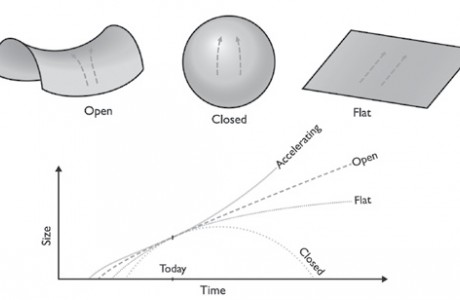
\includegraphics[width=0.8\textwidth]{scale_factor_various_model}
    \caption{Top: the three spatial geometries --- open (negative curvature), closed (positive curvature), and flat. Bottom: the scale factor $a(t)$ as a function of time for closed, flat, open, and accelerating cosmological models. The closed universe recollapses in a Big Crunch, while the open and flat cases expand forever. An accelerating universe (driven by a cosmological constant) overtakes all decelerating models at late times.}
    \label{fig:scale_factor_various}
\end{figure}

\subsection*{Parametric solutions: derivation}

We now solve the ODE exactly. Define the constant
\begin{equation}\label{eq:C_def}
    C \equiv \frac{8\pi G\rho_{m,0}}{3}\,,
\end{equation}
so that Eq.~\eqref{eq:fried_matter_k} can be written as
\begin{equation}\label{eq:adot_sq}
    \dot{a}^2 = \frac{C}{a} - k\,.
\end{equation}
This is a separable first-order ODE. Taking the positive root (expanding phase) and integrating from the Big Bang ($a=0$ at $t=0$):
\begin{equation}\label{eq:t_integral}
    t = \int_0^{a}\frac{da'}{\sqrt{C/a'-k}}\,.
\end{equation}
This integral cannot be evaluated in terms of elementary functions of $a$, but it \emph{can} be solved by introducing a parametric variable. We treat the closed and open cases in turn.

\medskip\noindent\textbf{Closed universe ($k=+1$): the cycloid.}

\medskip\noindent\emph{Step 1 --- Substitution.} The integrand in Eq.~\eqref{eq:t_integral} has the form $(C/a-1)^{-1/2}$, which vanishes at $a=C$ (the turnaround point $a_{\rm max}=C$ for $k=1$). This suggests a trigonometric substitution. Set
\begin{equation}\label{eq:closed_sub}
    a = \frac{C}{2}(1-\cos\eta)\,,
\end{equation}
so that $a$ ranges from $0$ (at $\eta=0$) to $C$ (at $\eta=\pi$) and back to $0$ (at $\eta=2\pi$). Differentiating:
\begin{equation}
    da = \frac{C}{2}\sin\eta\;d\eta\,.
\end{equation}

\medskip\noindent\emph{Step 2 --- Simplify $\sqrt{C/a-1}$.} Substituting Eq.~\eqref{eq:closed_sub}:
\begin{equation}
    \frac{C}{a} - 1 = \frac{C}{\frac{C}{2}(1-\cos\eta)} - 1
    = \frac{2}{1-\cos\eta} - 1
    = \frac{2-(1-\cos\eta)}{1-\cos\eta}
    = \frac{1+\cos\eta}{1-\cos\eta}\,.
\end{equation}
Using the half-angle identities $1+\cos\eta = 2\cos^2(\eta/2)$ and $1-\cos\eta = 2\sin^2(\eta/2)$:
\begin{equation}
    \frac{C}{a}-1 = \frac{\cos^2(\eta/2)}{\sin^2(\eta/2)}\,,
    \qquad\text{so}\qquad
    \sqrt{\frac{C}{a}-1} = \frac{\cos(\eta/2)}{\sin(\eta/2)}\,.
\end{equation}

\medskip\noindent\emph{Step 3 --- Compute $dt$.} From the ODE, $dt = da/\sqrt{C/a-k}$. With $k=1$:
\begin{align}
    dt &= \frac{da}{\sqrt{C/a-1}}
    = \frac{\frac{C}{2}\sin\eta\;d\eta}{\dfrac{\cos(\eta/2)}{\sin(\eta/2)}}
    = \frac{C}{2}\sin\eta\;\frac{\sin(\eta/2)}{\cos(\eta/2)}\;d\eta\,.
\end{align}
Now use the double-angle identity $\sin\eta = 2\sin(\eta/2)\cos(\eta/2)$:
\begin{align}
    dt &= \frac{C}{2}\cdot 2\sin(\eta/2)\cos(\eta/2)\cdot\frac{\sin(\eta/2)}{\cos(\eta/2)}\;d\eta
    = C\sin^2(\eta/2)\;d\eta\,.
\end{align}
Recognising $2\sin^2(\eta/2)=1-\cos\eta$, this can be written neatly as
\begin{equation}
    dt = \frac{C}{2}(1-\cos\eta)\;d\eta\,.
\end{equation}

\medskip\noindent\emph{Step 4 --- Integrate.} With $\eta=0$ at $t=0$:
\begin{equation}
    t = \frac{C}{2}\int_0^{\eta}(1-\cos\eta')\;d\eta' = \frac{C}{2}\bigl[\eta'-\sin\eta'\bigr]_0^{\eta} = \frac{C}{2}(\eta-\sin\eta)\,.
\end{equation}

\medskip\noindent\emph{Result.} For $k=+1$ and $a_{\rm max}=C$, the solution is
\begin{equation}
\boxed{
    a = \frac{a_{\rm max}}{2}(1-\cos\eta)\,,\qquad
    t = \frac{a_{\rm max}}{2}(\eta-\sin\eta)\,.}
    \label{eq:cycloid}
\end{equation}
This is the equation of a \textbf{cycloid} --- the curve traced by a point on the rim of a wheel of radius $a_{\rm max}/2$ rolling along the $t$-axis.

\medskip\noindent\emph{Check the limits:}
\begin{itemize}
    \item $\eta=0$: $a=0$, $t=0$ --- Big Bang.
    \item $\eta=\pi$: $a=a_{\rm max}=C$, $t=\frac{C}{2}(\pi-0)=\frac{\pi C}{2}$ --- maximum expansion; $\dot{a}=0$ (turnaround).
    \item $\eta=2\pi$: $a=0$, $t=\pi C$ --- Big Crunch. The total lifetime of the universe is $\pi C = \pi a_{\rm max}$.
\end{itemize}

\medskip\noindent\textbf{Open universe ($k=-1$): the hyperbolic solution.}

\medskip\noindent The derivation follows the same logic, with trigonometric functions replaced by their hyperbolic counterparts. With $k=-1$, the ODE becomes $\dot{a}^2=C/a+1$, and the right-hand side is always positive --- there is no turnaround.

\medskip\noindent\emph{Step 1 --- Substitution.} Set
\begin{equation}\label{eq:open_sub}
    a = \frac{C}{2}(\cosh\eta - 1)\,,
\end{equation}
so that $a=0$ at $\eta=0$ and $a$ increases monotonically. Differentiating:
\begin{equation}
    da = \frac{C}{2}\sinh\eta\;d\eta\,.
\end{equation}

\medskip\noindent\emph{Step 2 --- Simplify $\sqrt{C/a+1}$.} Substituting Eq.~\eqref{eq:open_sub}:
\begin{equation}
    \frac{C}{a}+1 = \frac{2}{\cosh\eta-1}+1 = \frac{2+(\cosh\eta-1)}{\cosh\eta-1} = \frac{1+\cosh\eta}{\cosh\eta-1}\,.
\end{equation}
Using the hyperbolic half-angle identities $1+\cosh\eta = 2\cosh^2(\eta/2)$ and $\cosh\eta-1=2\sinh^2(\eta/2)$:
\begin{equation}
    \sqrt{\frac{C}{a}+1} = \frac{\cosh(\eta/2)}{\sinh(\eta/2)}\,.
\end{equation}

\medskip\noindent\emph{Step 3 --- Compute $dt$.}
\begin{align}
    dt &= \frac{da}{\sqrt{C/a+1}}
    = \frac{\frac{C}{2}\sinh\eta}{\dfrac{\cosh(\eta/2)}{\sinh(\eta/2)}}\;d\eta
    = \frac{C}{2}\sinh\eta\;\frac{\sinh(\eta/2)}{\cosh(\eta/2)}\;d\eta\,.
\end{align}
Using $\sinh\eta = 2\sinh(\eta/2)\cosh(\eta/2)$:
\begin{align}
    dt &= \frac{C}{2}\cdot 2\sinh(\eta/2)\cosh(\eta/2)\cdot\frac{\sinh(\eta/2)}{\cosh(\eta/2)}\;d\eta
    = C\sinh^2(\eta/2)\;d\eta\,.
\end{align}
Since $2\sinh^2(\eta/2) = \cosh\eta-1$:
\begin{equation}
    dt = \frac{C}{2}(\cosh\eta-1)\;d\eta\,.
\end{equation}

\medskip\noindent\emph{Step 4 --- Integrate.}
\begin{equation}
    t = \frac{C}{2}\int_0^{\eta}(\cosh\eta'-1)\;d\eta' = \frac{C}{2}\bigl[\sinh\eta'-\eta'\bigr]_0^{\eta} = \frac{C}{2}(\sinh\eta-\eta)\,.
\end{equation}

\medskip\noindent\emph{Result.} Defining $a_0\equiv C = 8\pi G\rho_{m,0}/3$ for the open case:
\begin{equation}
\boxed{
    a = \frac{a_0}{2}(\cosh\eta-1)\,,\qquad
    t = \frac{a_0}{2}(\sinh\eta-\eta)\,.}
    \label{eq:hyperbolic}
\end{equation}

\medskip\noindent\emph{Check the limits:}
\begin{itemize}
    \item $\eta=0$: $a=0$, $t=0$ --- Big Bang.
    \item $\eta\to\infty$: $\cosh\eta\approx\sinh\eta\approx\frac{1}{2}e^\eta$, so $a\approx\frac{C}{4}e^\eta$ and $t\approx\frac{C}{4}e^\eta$. Thus $a\propto t$ --- the universe coasts at constant velocity, as predicted by the qualitative analysis.
\end{itemize}


\subsection{Radiation-Dominated Universe}

For matter, the energy in a comoving volume is constant: mass is conserved. For radiation, something different happens. Consider a box of photons expanding with the universe.

There are two effects:

\medskip\noindent\textbf{Effect 1: Dilution.} Just like matter, the number density of photons decreases as the volume grows. If we have $N$ photons in a comoving volume $V\propto a^3$, the number density goes as $n\propto a^{-3}$.

\medskip\noindent\textbf{Effect 2: Redshift.} Unlike massive particles, each photon also loses energy as the universe expands. A photon's wavelength stretches with the scale factor:
\begin{equation}
    \lambda \propto a\,.
\end{equation}
Since the energy of a photon is $E=hc/\lambda$, each photon's energy decreases as
\begin{equation}
    E_\gamma \propto \frac{1}{a}\,.
\end{equation}
This is the cosmological redshift. It is not a Doppler effect --- it is the stretching of space itself stretching the wavelength of the photon.

\medskip\noindent\textbf{Combined effect:} The radiation energy density is (number density) $\times$ (energy per photon):
\begin{equation}
    \rho_r \propto n\cdot E_\gamma \propto a^{-3}\cdot a^{-1} = a^{-4}\,.
\end{equation}
So:
\begin{equation}
\boxed{\rho_r(t) = \frac{\rho_{r,0}}{a^4(t)}\,.}
\end{equation}
Radiation dilutes faster than matter by one extra power of $a$, due to the redshift.


With $k=0$ and radiation only:
\begin{equation}
    H^2 = \frac{8\pi G}{3}\,\frac{\rho_{r,0}}{a^4}\,.
\end{equation}
Taking the square root:
\begin{equation}
    \dot{a} = B\,a^{-1}\,,
\end{equation}
where $B\equiv\sqrt{8\pi G\rho_{r,0}/3}$. Separating variables:
\begin{equation}
    a\,da = B\,dt\,.
\end{equation}
Integrating:
\begin{equation}
    \frac{1}{2}\,a^2 = Bt\,.
\end{equation}
Solving for $a$:
\begin{equation}
\boxed{a(t) = (2Bt)^{1/2} \propto t^{1/2}\,.}
\end{equation}

\subsection*{Properties of the radiation-dominated solution}

The Hubble parameter is
\begin{equation}
    H(t) = \frac{\dot{a}}{a} = \frac{1}{2t}\,,
\end{equation}
so the age of a radiation-dominated universe would be
\begin{equation}
    t_0 = \frac{1}{2H_0}\,,
\end{equation}
even younger than the matter-dominated case ($t_0=2/(3H_0)$). The expansion decelerates faster because radiation has a larger effective gravitational mass ($\rho+3p=2\rho$ for radiation, versus $\rho$ for matter).

The deceleration parameter is
\begin{equation}
    q = 1\,,
\end{equation}
compared to $q=1/2$ for matter. The stronger deceleration reflects the extra pressure contribution to gravity.


\subsection{Comparing Matter and Radiation}

\subsection*{Which dominates when?}

Since $\rho_m\propto a^{-3}$ and $\rho_r\propto a^{-4}$, their ratio is
\begin{equation}
    \frac{\rho_r}{\rho_m} = \frac{\rho_{r,0}}{\rho_{m,0}}\,\frac{1}{a}\,.
\end{equation}
At early times ($a\ll 1$), radiation dominates. At late times ($a\gg a_{\rm eq}$), matter dominates. The crossover occurs at matter--radiation equality:
\begin{equation}
    a_{\rm eq} = \frac{\rho_{r,0}}{\rho_{m,0}}\,.
\end{equation}
Using observed values, $a_{\rm eq}\approx 1/3400$, corresponding to a redshift $z_{\rm eq}\approx 3400$ and a temperature $T_{\rm eq}\approx 9500$ K. This is shortly before the epoch of recombination ($z\approx 1100$).

\subsection*{The thermal history in brief}

The temperature of the radiation bath scales as
\begin{equation}
    T \propto \frac{1}{a}\,,
\end{equation}
because the typical photon energy $E\propto 1/a$, and for a thermal distribution $E\sim k_B T$. This means:
\begin{itemize}
    \item Early universe ($a\ll a_{\rm eq}$): radiation-dominated, $a\propto t^{1/2}$, $T\propto t^{-1/2}$.
    \item After equality ($a\gg a_{\rm eq}$): matter-dominated, $a\propto t^{2/3}$, $T\propto t^{-2/3}$.
\end{itemize}

\begin{figure}[H]
    \centering
    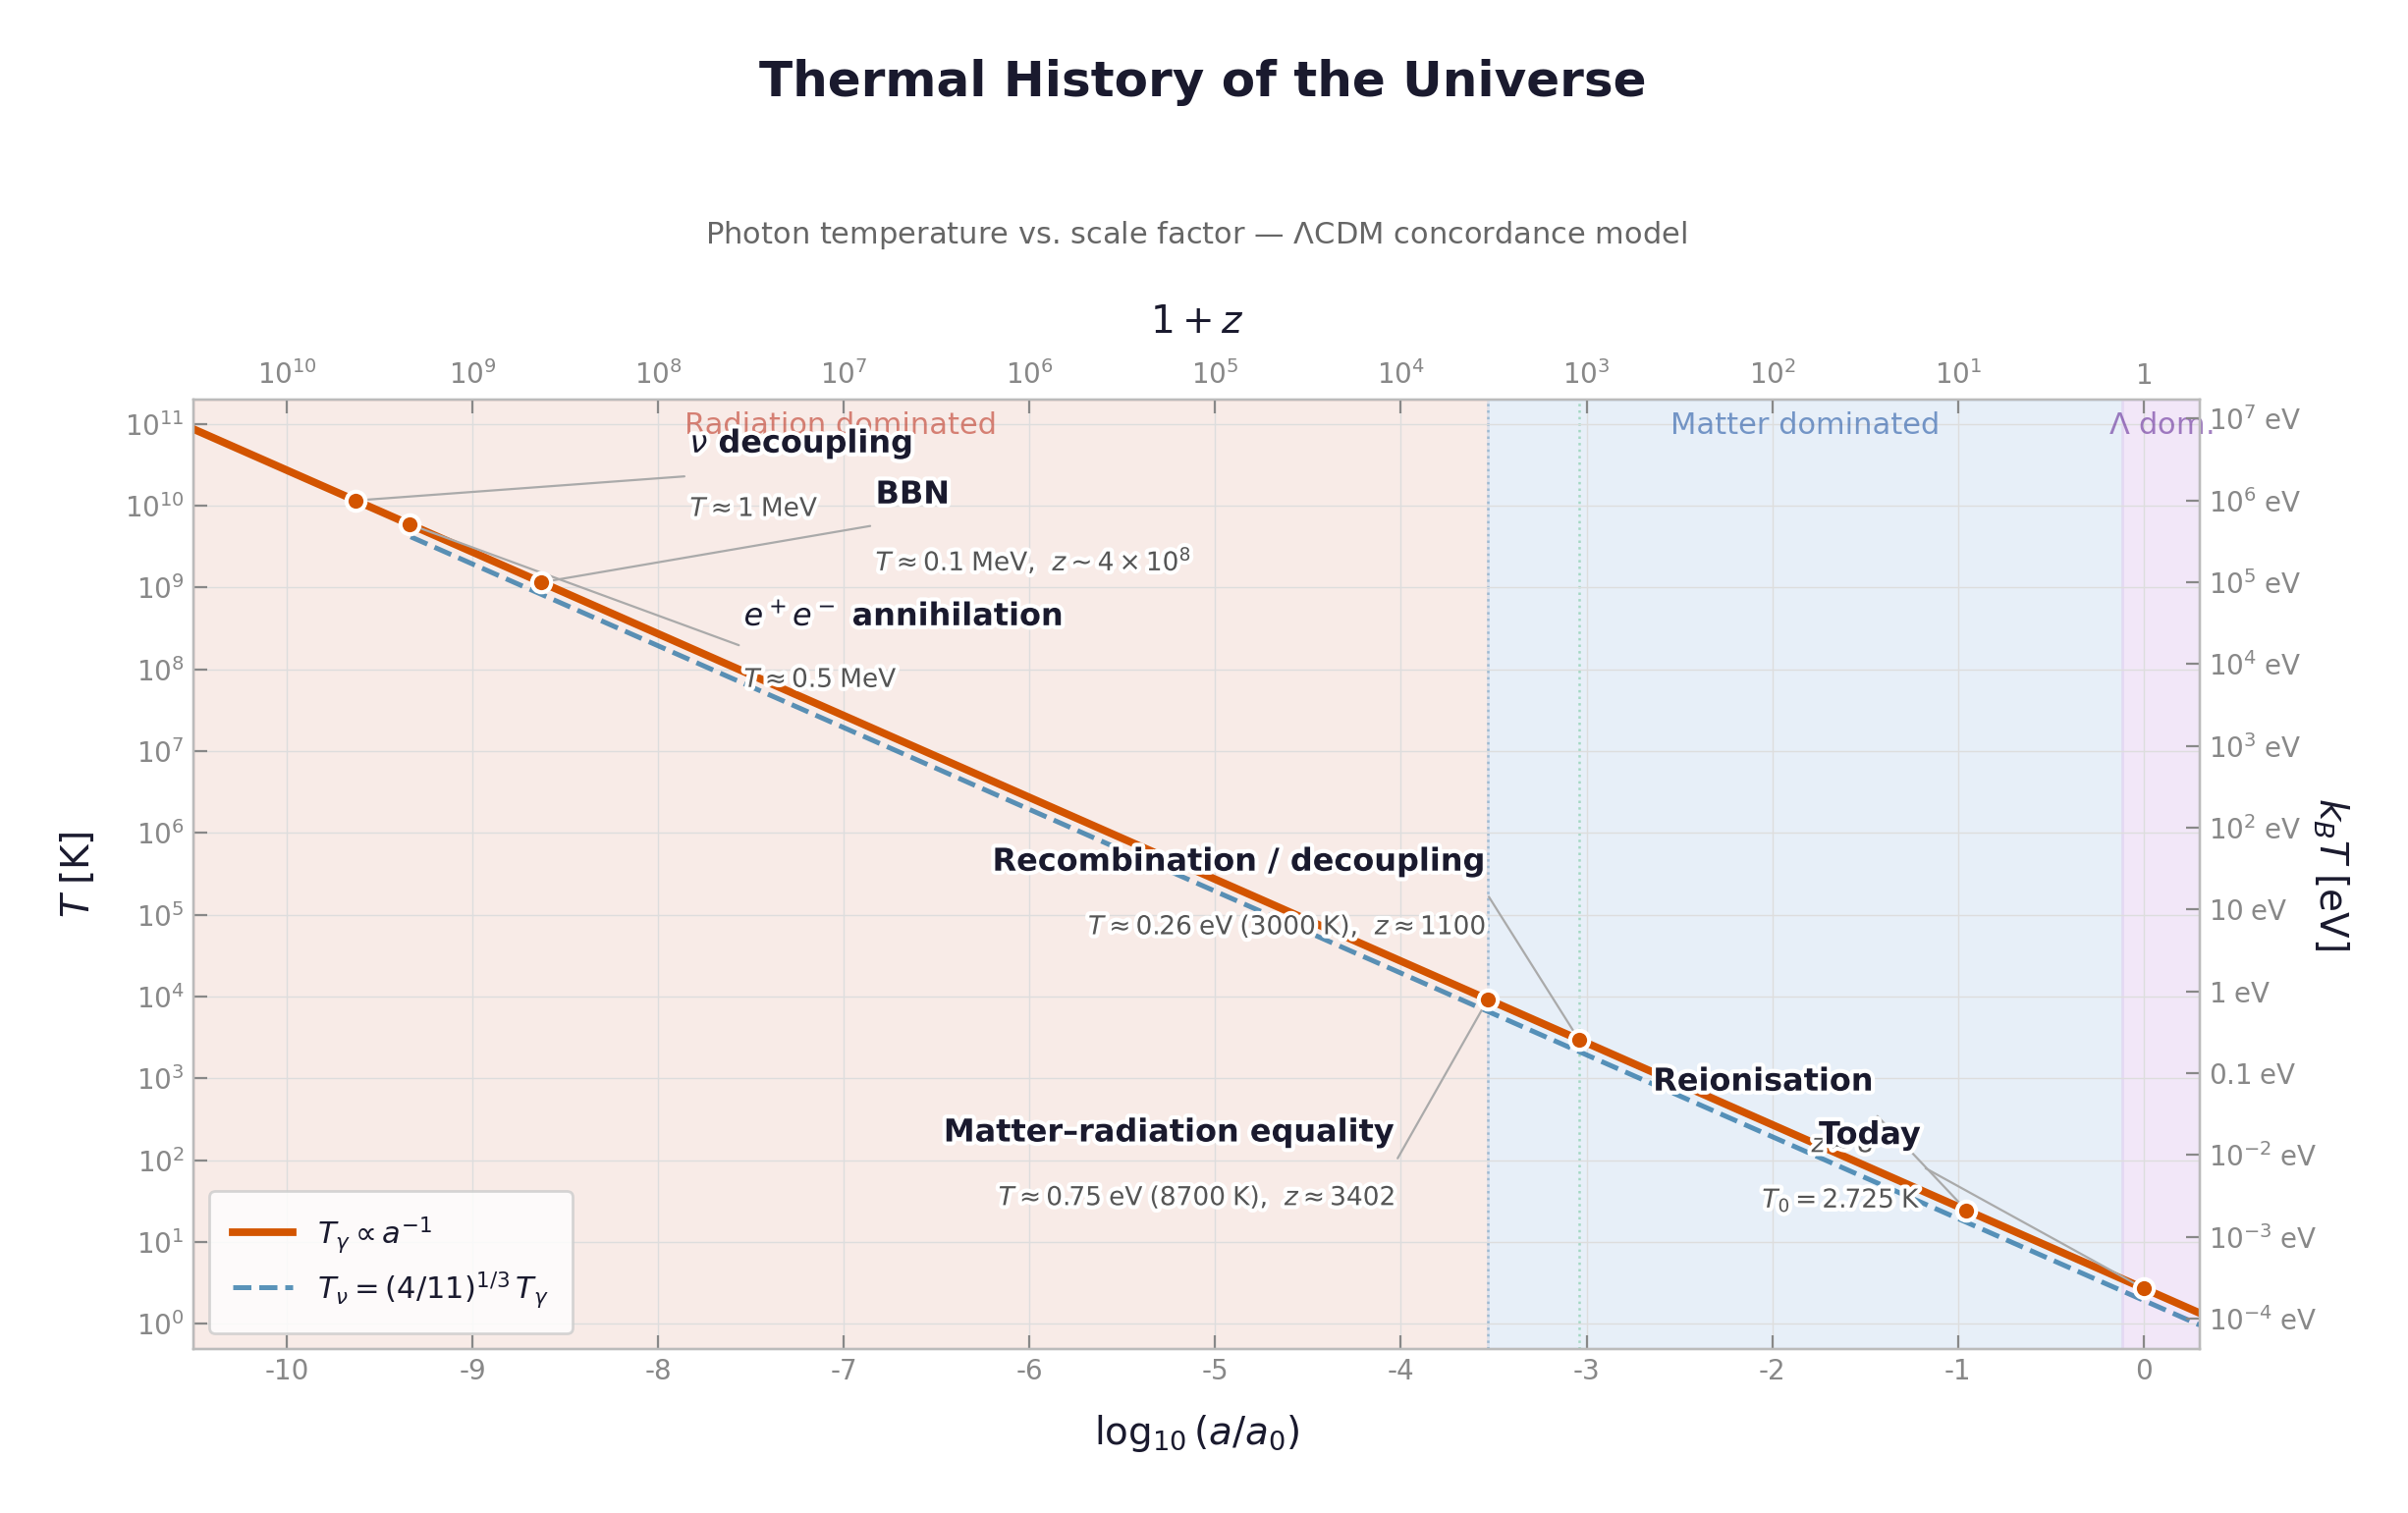
\includegraphics[width=0.85\textwidth]{thermal_history_light}
    \caption{Thermal history of the Universe in the $\Lambda$CDM concordance model. The photon temperature $T_\gamma \propto a^{-1}$ (solid orange) and the neutrino temperature $T_\nu = (4/11)^{1/3}\,T_\gamma$ (dashed) are shown as a function of scale factor. Key events are labelled: neutrino decoupling, Big Bang nucleosynthesis (BBN), $e^+e^-$ annihilation, recombination/decoupling, matter--radiation equality, reionisation, and the present day. Shaded bands indicate the radiation-dominated (red), matter-dominated (blue), and $\Lambda$-dominated (purple) epochs.}
    \label{fig:thermal_history}
\end{figure}

\subsection*{Summary of single-component flat universes}

The general pattern is worth seeing together. For a single component with equation of state $p=w\rho$, the continuity equation gives $\rho\propto a^{-3(1+w)}$, and the Friedmann equation gives:
\begin{equation}
    a(t) \propto t^{2/[3(1+w)]}\,,\qquad H = \frac{2}{3(1+w)}\,\frac{1}{t}\,,\qquad q = \frac{1+3w}{2}\,.
\end{equation}
Specific cases:

\medskip
\begin{center}
\begin{tabular}{lcccccc}
\hline\hline
Component & $w$ & $\rho\propto$ & $a(t)\propto$ & $H(t)$ & $q$ & Age \\
\hline
Matter    & $0$    & $a^{-3}$ & $t^{2/3}$ & $\dfrac{2}{3t}$ & $\dfrac{1}{2}$ & $\dfrac{2}{3H_0}$ \\[10pt]
Radiation & $1/3$  & $a^{-4}$ & $t^{1/2}$ & $\dfrac{1}{2t}$ & $1$ & $\dfrac{1}{2H_0}$ \\[10pt]
Curvature$^*$ & $-1/3$ & $a^{-2}$ & $t^{1}$ & $\dfrac{1}{t}$ & $0$ & $\dfrac{1}{H_0}$ \\[10pt]
$\Lambda$ & $-1$ & $a^{0}$ & $e^{Ht}$ & const & $-1$ & $\infty$ \\[4pt]
\hline\hline
\end{tabular}
\end{center}

\medskip
\noindent$^*$The ``curvature'' row treats the $k/a^2$ term as an effective fluid with $w=-1/3$. This is the empty, coasting Milne universe.

The cosmological constant case ($w=-1$) is qualitatively different: $\rho_\Lambda=\text{const}$, the expansion is exponential, and the universe accelerates ($q<0$), as derived in the previous section.

\begin{figure}[H]
    \centering
    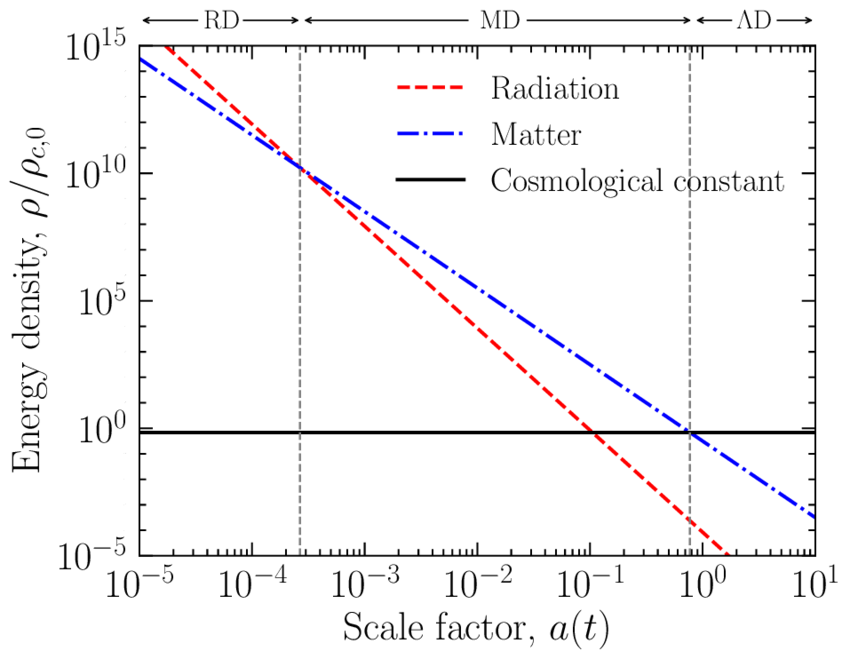
\includegraphics[width=0.75\textwidth]{rho_vs_a}
    \caption{Energy density (in units of today's critical density $\rho_{c,0}$) as a function of scale factor for radiation ($\rho_r \propto a^{-4}$), matter ($\rho_m \propto a^{-3}$), and the cosmological constant ($\rho_\Lambda = \text{const}$). Vertical dashed lines mark the matter--radiation equality ($a_{\rm eq} \approx 3 \times 10^{-4}$) and the matter--$\Lambda$ equality ($a \approx 0.75$). The labels RD, MD, and $\Lambda$D indicate the radiation-, matter-, and $\Lambda$-dominated epochs.}
    \label{fig:rho_vs_a}
\end{figure}


\subsection{A General Formula: the Friedmann Integral}

For a flat universe containing both matter and radiation (and potentially a cosmological constant), the Friedmann equation is
\begin{equation}
    H^2 = H_0^2\!\left[\frac{\Omega_{r,0}}{a^4} + \frac{\Omega_{m,0}}{a^3} + \Omega_{\Lambda,0}\right],
\end{equation}
where $\Omega_{r,0}+\Omega_{m,0}+\Omega_{\Lambda,0}=1$ for a flat universe. The age of the universe can be written as the integral
\begin{equation}
    t_0 = \frac{1}{H_0}\int_0^1 \frac{da}{\sqrt{\Omega_{r,0}\,a^{-2} + \Omega_{m,0}\,a^{-1} + \Omega_{\Lambda,0}\,a^2}}\,.
\end{equation}
This integral generally requires numerical evaluation, but reduces to the analytic solutions above in the single-component limits. Using the observed values $\Omega_{m,0}\approx 0.3$, $\Omega_{\Lambda,0}\approx 0.7$, and $\Omega_{r,0}\approx 10^{-4}$, one obtains $t_0\approx 13.8$ Gyr --- the correct age of the universe. The cosmological constant contributes significantly to increasing the age compared to the matter-only estimate of $\sim 9$ Gyr.



% --- Lecture 3 ----------------------------------------------------------
%\input{sections/lecture_03_dark_energy}

% --- Lecture 4 ----------------------------------------------------------
%\input{sections/lecture_04_dark_matter}

% --- Lecture 5 ----------------------------------------------------------
%\input{sections/lecture_05_linear_structure}

% --- Lecture 6 ----------------------------------------------------------
%\input{sections/lecture_06_nonlinear_structure}

% --- Lecture 7 ----------------------------------------------------------
%\input{sections/lecture_07_thermal_history}

% --- Lecture 8 ----------------------------------------------------------
%\input{sections/lecture_08_cmb}

% --- Lecture 9 ----------------------------------------------------------
%\input{sections/lecture_09_bao}

% --- Lecture 10 ---------------------------------------------------------
%\input{sections/lecture_10_galaxy_clustering}

% --- Lecture 12 ---------------------------------------------------------
%\input{sections/lecture_12_galaxy_clusters}

% --- Lecture 13 ---------------------------------------------------------
%\input{sections/lecture_13_gravitational_lensing}

% --- Lecture 14 ---------------------------------------------------------
%\input{sections/lecture_14_combined_probes}

% --- Lecture 15 ---------------------------------------------------------
%\input{sections/lecture_15_alternative_models}

\end{document}
